\section{Preliminary Results and Findings}
\label{sec:preliminary_results}

This section presents the results obtained from training a subset of the algorithms discussed in section \ref{subsec:algorithm_selection}. The selected algorithms include five DQN-based methods — DQN, Double DQN, Prioritized Experience Replay, Dueling DQN, and C51 — as well as three policy-based methods: REINFORCE, PPO, and SAC. Soft Actor Critic was preferred to DDPG and TD3 because it can simply be seen as a variation that works with a stochastic policy, but is more easily adapted to a discrete action space.

We first describe necessary modifications to the experiment setup, followed by a detailed analysis of each algorithm's performance and emissions. The results are then compared inter-algorithm families and across them.

\subsection{Experiment Setup Adjustments}
\label{subsec:exp_setup_adjustments}
During initial training attempts, some adjustments were required to ensure reliable performance and energy tracking. One key reason for this was that employing CodeCarbon as a (next-)real-time emissions tracking tool significantly slowed down training (by a factor of 20 or more). As a result, we opted to record only total emissions at the end of training rather than tracking them continously. This adjustment allowed us to obtain meaningful comparisons without excessively increasing training time.

In addition to this, on Windows, CodeCarbon's CPU energy tracking relies on the Intel Power Gadget, which has been deprecated for several years. Furthermore, it does not support Intel Performance Counter Monitor (Intel PCM), the official successor to the Power Gadget. In such cases, CodeCarbon switches to a fallback mode, directly quoting from their documentation:
\begin{quoting}
	\begin{itemize}
		\item It will first detect which CPU hardware is currently in use, and then map it to a data source listing 2000+ Intel and AMD CPUs and their corresponding thermal design powers (TDPs).
		
		\item If the CPU is not found in the data source, a global constant will be applied. CodeCarbon assumes that 50\% of the TDP will be the average power consumption to make this approximation.
		
		\item We could not find any good resource showing statistical relationships between TDP and average power, so we empirically tested that 50\% is a decent approximation.
	\end{itemize}
\end{quoting}

This approach should provide reasonable estimates for our project, since most of the workload is on the GPU, while the rest is mostly constant across the algorithms (like the environment simulations). This being said, one instance where this limitation may have had an impact is in tracking the Proximal Policy Optimization (PPO) algorithm, that employs a relatively small neural network but requires more CPU and RAM processing, the latter also explicitly stated to not be tracked satisfactorily by CodeCarbon.

Additionally, Weights \& Biases collects system data during training, and while it tracks GPU energy consumption in kWh, it also does not do the same for CPU and RAM. As a result, while we can obtain excellent emissions estimates for the GPU, CPU and RAM energy tracking remains imprecise due to the aforementioned limitations. Consequently, energy consumption analyses must be interpreted with an understanding of these constraints.

\subsection{DQN-Based Algorithms}
We present the results for the five different DQN-based algorithms. Each algorithm is analyzed individually before an overall comparison.

\subsubsection{Deep Q-Network (DQN Baseline)}
\label{subsubsec:dqn_baseline}

\paragraph{(Hyper)Parameters}
Table~\ref{tab:dqn_hyperparams} summarizes the main hyperparameters used for our DQN baseline.  
\texttt{env\_id} and \texttt{seed} varied across runs (eight Atari games $\times$ four seeds), 
while the rest remained unchanged. Note in particular that \texttt{buffer\_size} and 
\texttt{learning\_starts} have been reduced relative to their usual millions-step values to 
accommodate the shorter 100k-step regime.

\begin{table}
	\caption{Key hyperparameters for the DQN baseline. Only \texttt{env\_id} and \texttt{seed} change across runs.}
	\label{tab:dqn_hyperparams}
	\centering
	\begin{tabular}{ll}
		\toprule
		\textbf{Parameter} & \textbf{Value} \\
		\midrule
		\texttt{exp\_name}                & dqn\_atari \\
		\texttt{seed}                     & 1..4 \\
		\texttt{torch\_deterministic}     & True \\
		\texttt{cuda}                     & True \\
		\texttt{track}                    & True \\
		\texttt{wandb\_project\_name}     & rlsb \\
		\texttt{capture\_video}           & False \\
		\texttt{save\_model}              & True \\
		\texttt{upload\_model}            & False \\
		\texttt{env\_id}                  & e.g.\ AlienNoFrameskip-v4 \\
		\texttt{total\_timesteps}         & 100000 \\
		\texttt{learning\_rate}           & 0.0001 \\
		\texttt{num\_envs}                & 1 \\
		\texttt{buffer\_size}             & 10000 \\
		\texttt{gamma}                    & 0.99 \\
		\texttt{tau}                      & 1.0 \\
		\texttt{target\_network\_frequency} & 1000 \\
		\texttt{batch\_size}             & 32 \\
		\texttt{start\_e}, \texttt{end\_e} & 1.0 $\to$ 0.01 \\
		\texttt{exploration\_fraction}    & 0.1 \\
		\texttt{learning\_starts}         & 1000 \\
		\texttt{train\_frequency}         & 4 \\
		\bottomrule
	\end{tabular}
\end{table}

\paragraph{Hyperparameter Tuning}
We began with the \emph{CleanRL} defaults (similar to Mnih~et~al.'s original DQN~\cite{mnih:atari}) and
scaled down parameters tied to a large number of environment interactions. For instance,
\texttt{buffer\_size} was tested at \{10k, 20k\}, and \texttt{learning\_starts} 
at \{800, 1000, 2000, 5000\}. Empirically, a buffer of 10k 
and \texttt{learning\_starts} of 1000 provided the best trade-off between stability 
and performance in the 100k-step setting. We kep $\tau$ equal to \num{1} for consistency with the original work.
This parameter regulates the update of the target network weights by controlling the interpolation between those of the 
current Q-network and target network, following the update rule:
$$
\theta_{\text{target}} = \tau \theta + (1 - \tau) \theta_{\text{target}}
$$
where $\theta_{\text{target}}$ are the weights of the target network and $\theta$ are the ones of the q-network.
For \(\tau = 1\), the target network is completely overwritten by the Q-network 
every time it's updated, as done in the original DQN.

\paragraph{Training Dynamics (Aggregated Over 32 Runs)}
Figure~\ref{fig:dqn_episodic_length} shows that episodes usually last in the 3000--4000 step range, 
but certain runs or environments have early terminations (very short episodes) or extremely long ones (around 8000 steps).  
Figure~\ref{fig:dqn_sps} indicates that, computationally, training stabilizes at a solid 
\(\sim\)170 steps per second on average, though environment differences introduce some variance.

\begin{figure}
	\centering
	\subfloat[][\emph{Aggregated episodic length for DQN over 100k steps (interpolation across 32 runs). 
		The mean hovers around 3500--4000 steps, 
		while the min--max envelope extends from near 0 to over 8000.}]
	{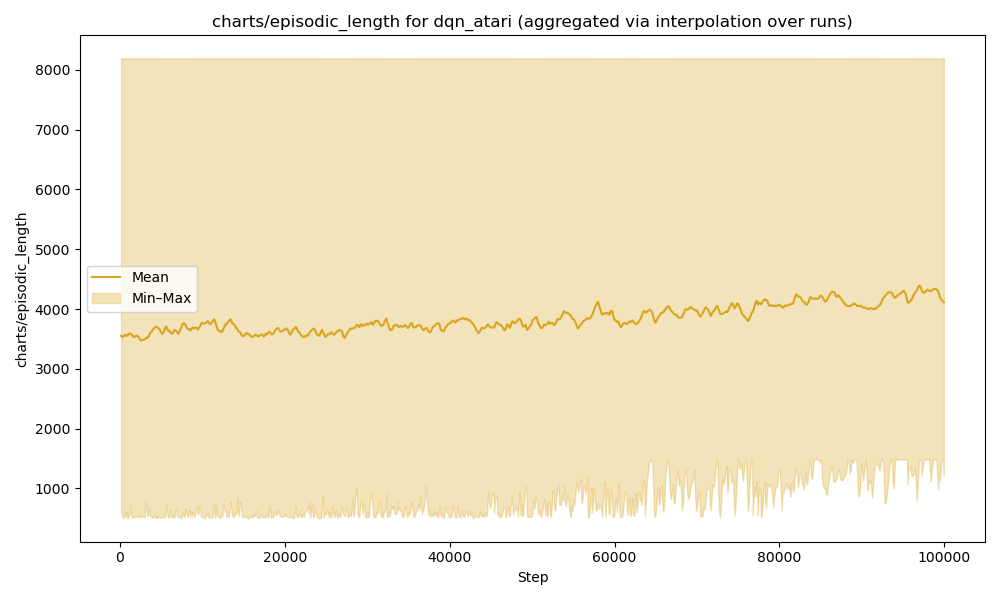
\includegraphics[width=.45\textwidth]{figures/dqn/charts_episodic_length_dqn_atari.png} \label{fig:dqn_episodic_length}} \quad
	\subfloat[][\emph{Steps per second (SPS) for DQN. After an initial ramp-up, 
		the mean SPS stabilizes around 170--180, 
		with some runs dipping as low as 20 or spiking above 200.}]
	{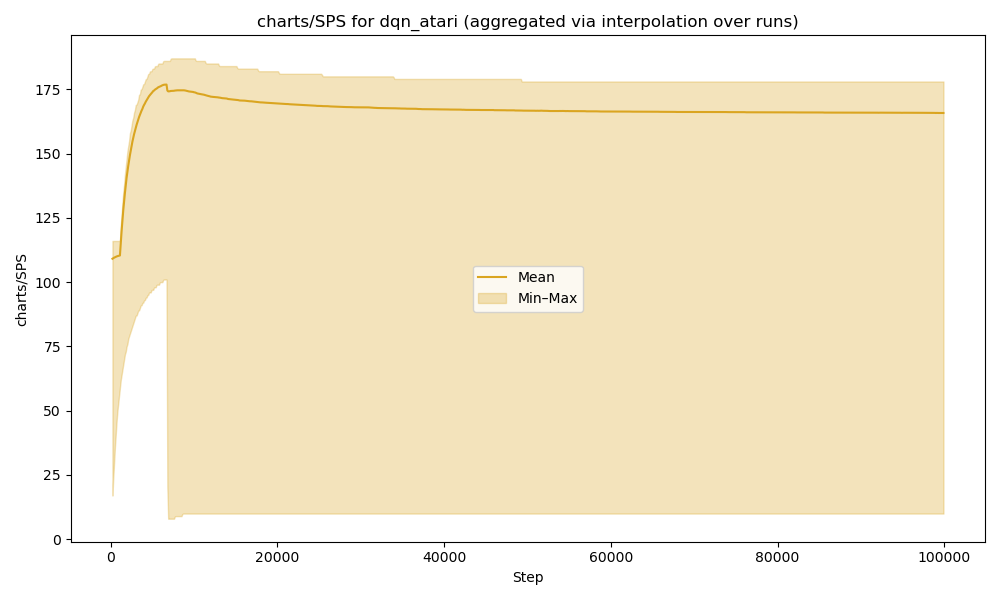
\includegraphics[width=.45\textwidth]{figures/dqn/charts_SPS_dqn_atari.png} \label{fig:dqn_sps}} \\ 
	\subfloat[][\emph{Estimated Q-values (\texttt{losses/q\_values}) for DQN 
		(aggregated over 32 runs). 
		The mean Q-value climbs from near 0 up to \(\sim\)4--5, 
		while some runs exceed 10.}]
	{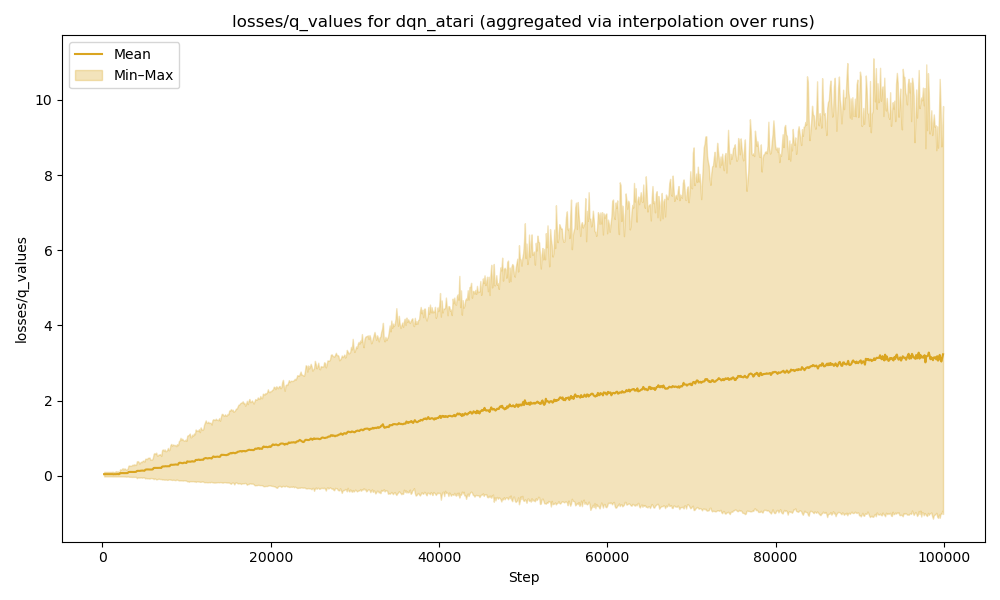
\includegraphics[width=.45\textwidth]{figures/dqn/losses_q_values_dqn_atari.png} \label{fig:dqn_q_values}} \quad
	\subfloat[][\emph{TD loss (\texttt{losses/td\_loss}) for DQN. 
		Losses grow with training, reaching above 3.0 in some runs, 
		reflecting substantial variance near the final stages.}]
	{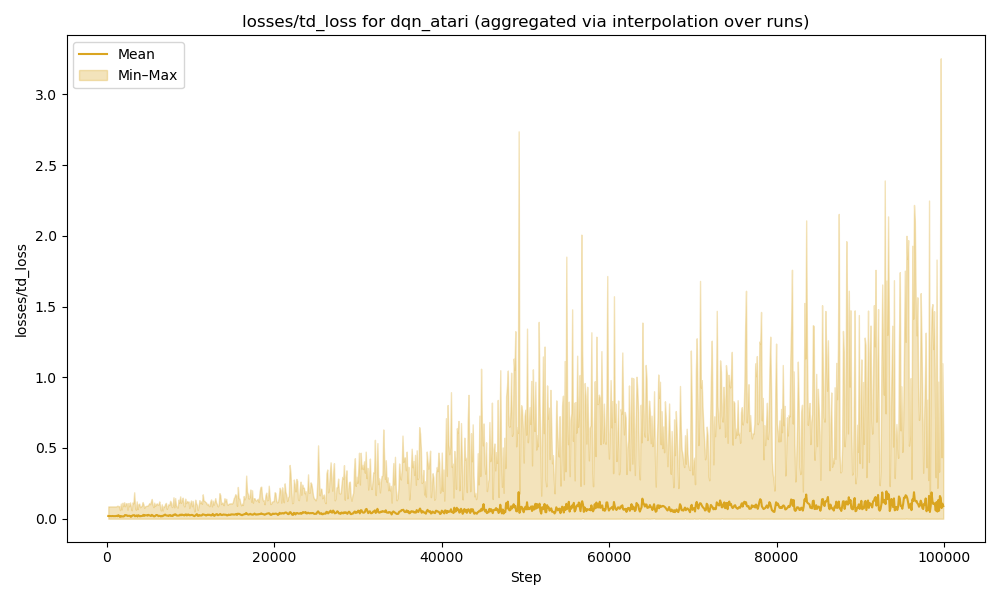
\includegraphics[width=.45\textwidth]{figures/dqn/losses_td_loss_dqn_atari.png} \label{fig:dqn_td_loss}}
	\caption{Performance metrics for DQN over 100k steps, aggregated across 32 runs.}
	\label{fig:dqn_subfigures}
\end{figure}

%
%\begin{figure}
%	\centering
%	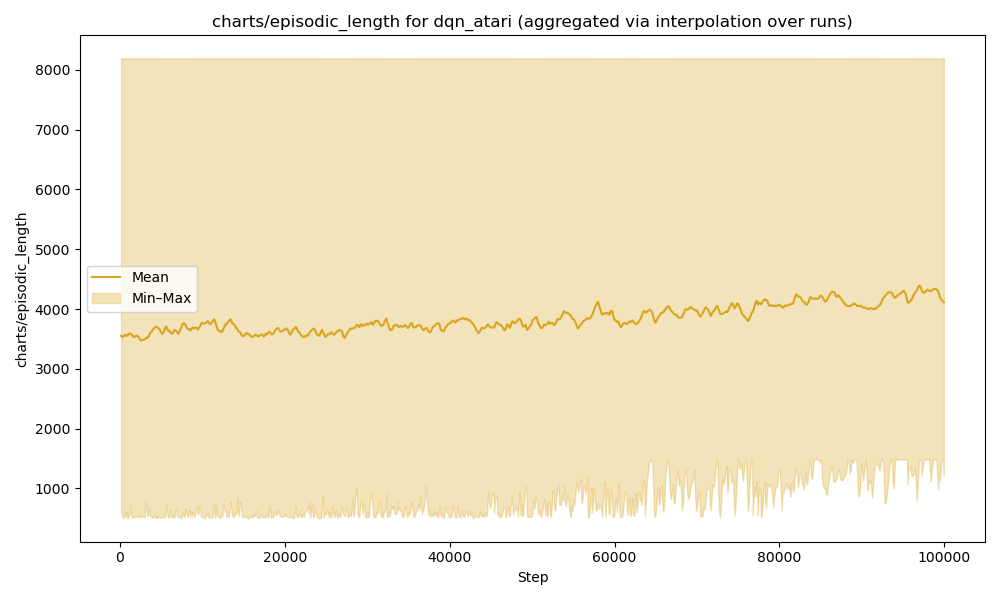
\includegraphics[width=0.6\textwidth]{figures/dqn/charts_episodic_length_dqn_atari.png}
%	\caption{Aggregated episodic length for DQN over 100k steps 
%		(interpolation across 32 runs). 
%		The mean hovers around 3500--4000 steps, 
%		while the min--max envelope extends from near 0 to over 8000.}
%	\label{fig:dqn_episodic_length}
%\end{figure}
%\begin{figure}
%	\centering
%	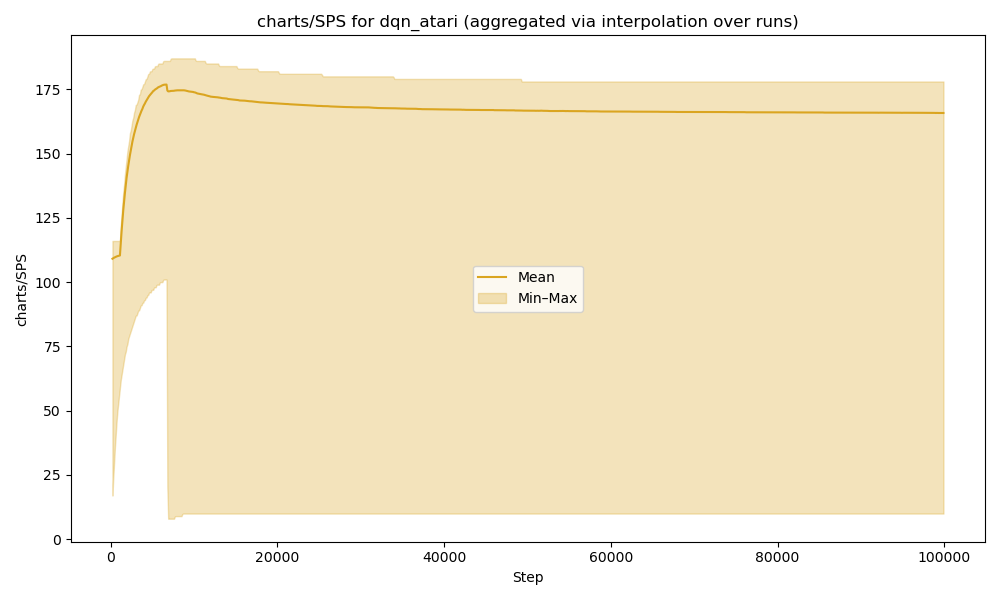
\includegraphics[width=0.6\textwidth]{figures/dqn/charts_SPS_dqn_atari.png}
%	\caption{Steps per second (SPS) for DQN. After an initial ramp-up, 
%		the mean SPS stabilizes around 170--180, 
%		with some runs dipping as low as 20 or spiking above 200.}
%	\label{fig:dqn_sps}
%\end{figure}
%\begin{figure}
%	\centering
%	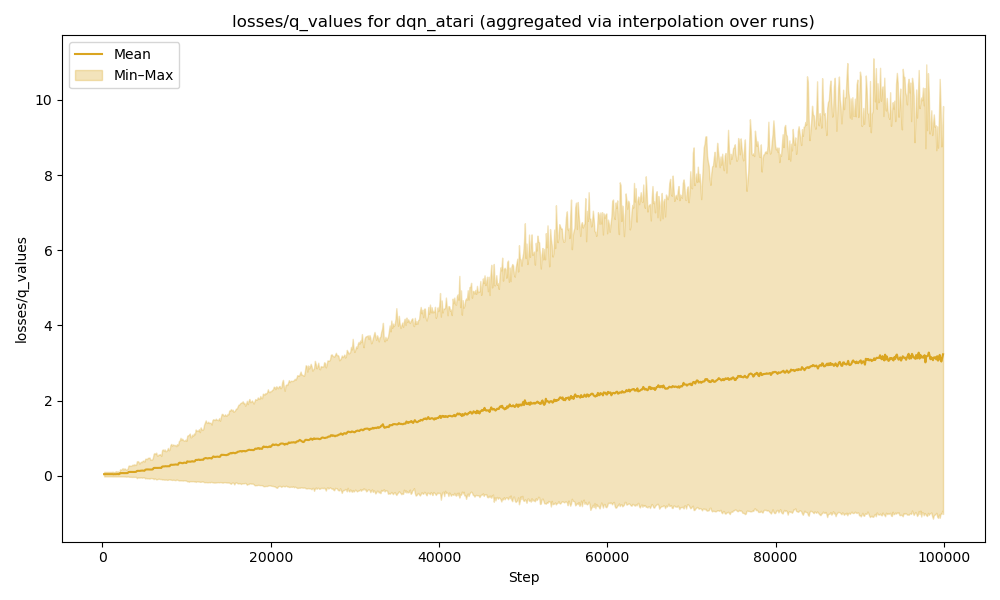
\includegraphics[width=0.6\textwidth]{figures/dqn/losses_q_values_dqn_atari.png}
%	\caption{Estimated Q-values (\texttt{losses/q\_values}) for DQN 
%		(aggregated over 32 runs). 
%		The mean Q-value climbs from near 0 up to \(\sim\)4--5, 
%		while some runs exceed 10.}
%	\label{fig:dqn_q_values}
%\end{figure}
%\begin{figure}
%	\centering
%	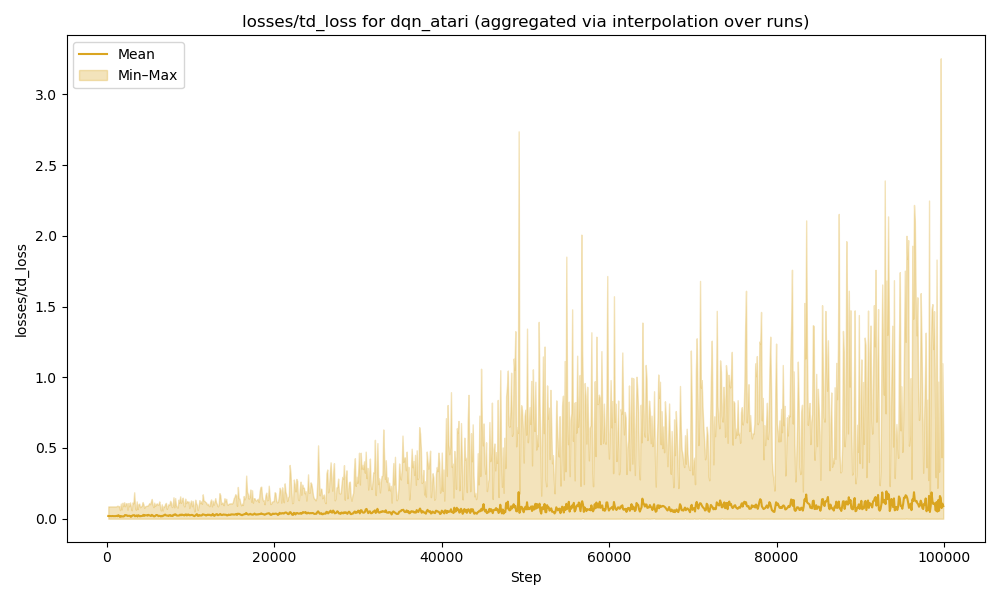
\includegraphics[width=0.6\textwidth]{figures/dqn/losses_td_loss_dqn_atari.png}
%	\caption{TD loss (\texttt{losses/td\_loss}) for DQN. 
%		Losses grow with training, reaching above 3.0 in some runs, 
%		reflecting substantial variance near the final stages.}
%	\label{fig:dqn_td_loss}
%\end{figure}

\paragraph{Q-Values and TD Loss}
Figures~\ref{fig:dqn_q_values} and \ref{fig:dqn_td_loss} show \texttt{losses/q\_values} and 
\texttt{losses/td\_loss}, respectively, across all runs.
On average, Q-values increase steadily, suggesting the network’s estimates 
of future returns keep growing with experience. However, 
the broad min--max band indicates some seeds or games diverge or plateau differently. 
The TD loss remains small in early training but spikes in certain runs, 
possibly due to volatile updates from the replay buffer once it’s partially filled.

\paragraph{Episodic Return (Human vs.\ Min--Max Normalized)}
We analyzed the collected episodic returns applying both the human normalization and min--max normalization schemes, as explained in section~\vref{subsubsec:normalization}.
Figures~\ref{fig:dqn_return_human} and \ref{fig:dqn_return_minmax} aggregate 
these returns across all 32 runs, while 
Figures~\ref{fig:dqn_return_pergame_human} and \ref{fig:dqn_return_pergame_minmax} 
show per-game curves.

\begin{figure}
	\centering
	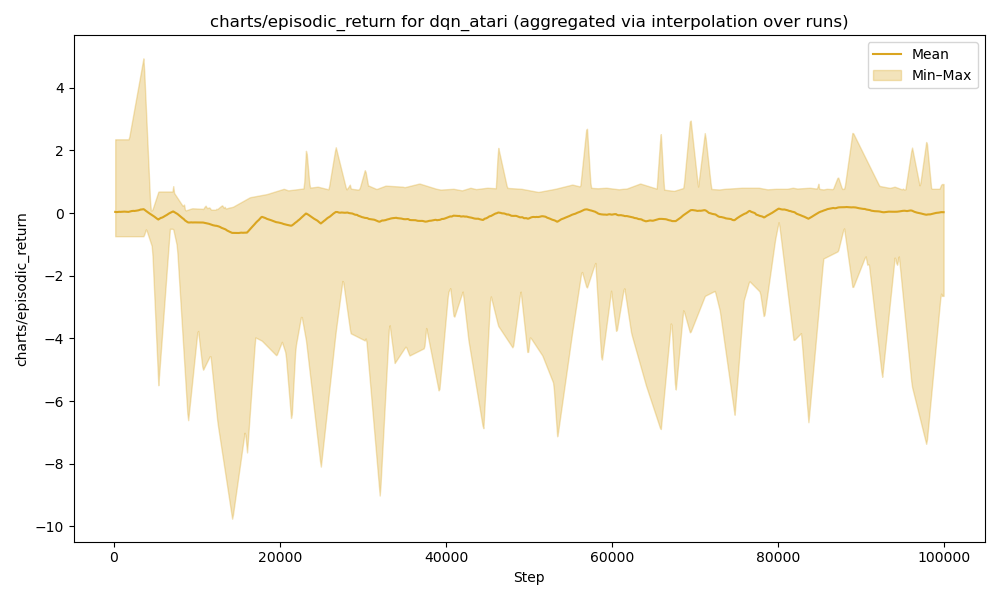
\includegraphics[width=0.6\textwidth]{figures/dqn/charts_episodic_return_human_dqn_atari.png}
	\caption{Aggregated DQN episodic return (human-normalized) 
		over 100k steps. The shaded region represents min--max variation.}
	\label{fig:dqn_return_human}
\end{figure}

\begin{figure}
	\centering
	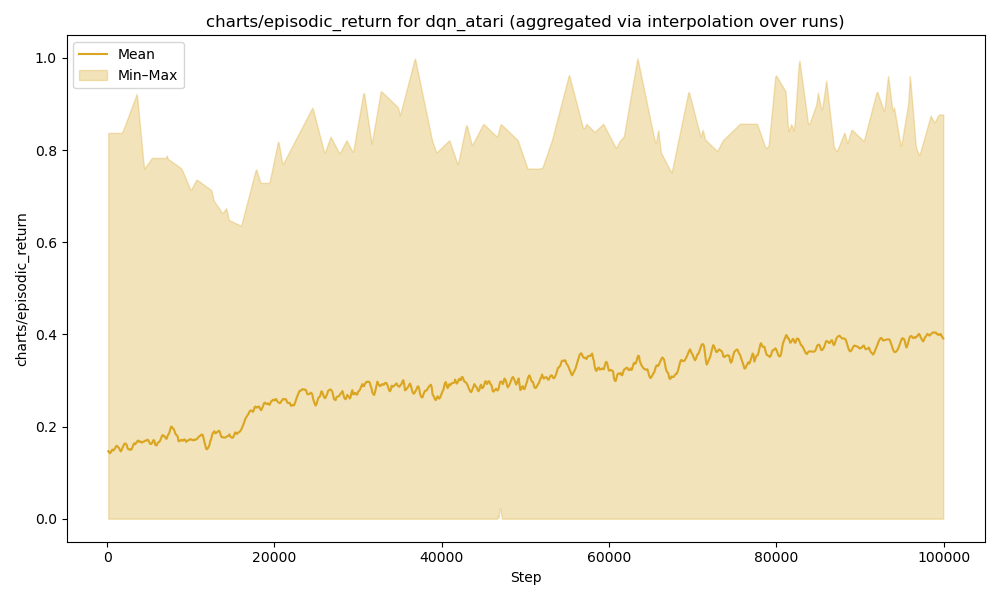
\includegraphics[width=0.6\textwidth]{figures/dqn/charts_episodic_return_minmax_dqn_atari.png}
	\caption{Aggregated DQN episodic return (min--max normalized).}
	\label{fig:dqn_return_minmax}
\end{figure}

In the human-normalized plot, the mean hovers near zero, 
occasionally dipping negative due to poor performance on certain games. 
In the min--max plot, the average climbs from near 0.2 to around 0.4--0.5 by the end, 
indicating moderate relative progress.

\begin{figure}
	\centering
	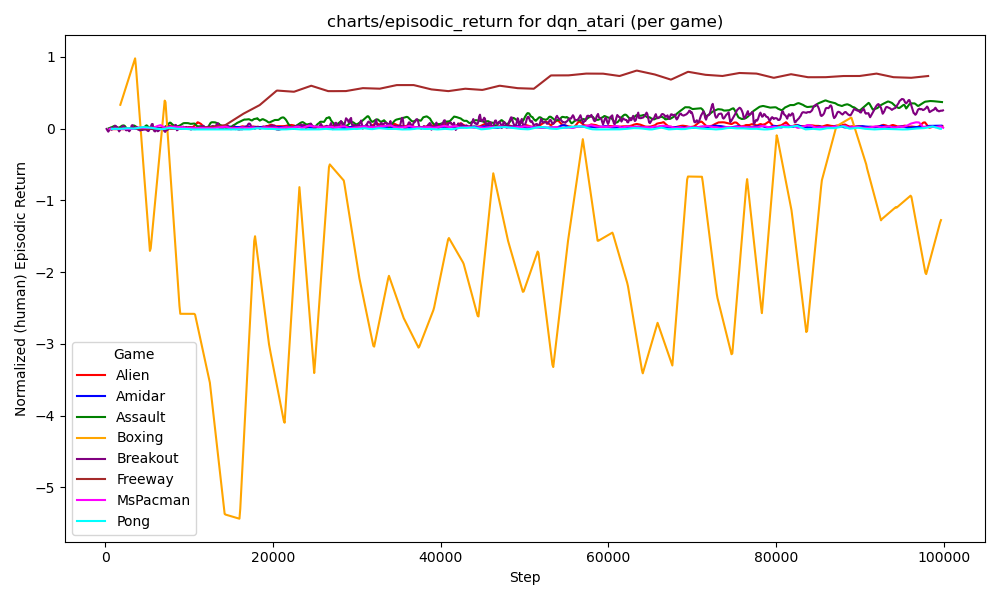
\includegraphics[width=0.6\textwidth]{figures/dqn/charts_episodic_return_per_game_human_dqn_atari.png}
	\caption{DQN returns (human-normalized) by game. Each line aggregates 
		four seeds for that specific environment.}
	\label{fig:dqn_return_pergame_human}
\end{figure}

\begin{figure}
	\centering
	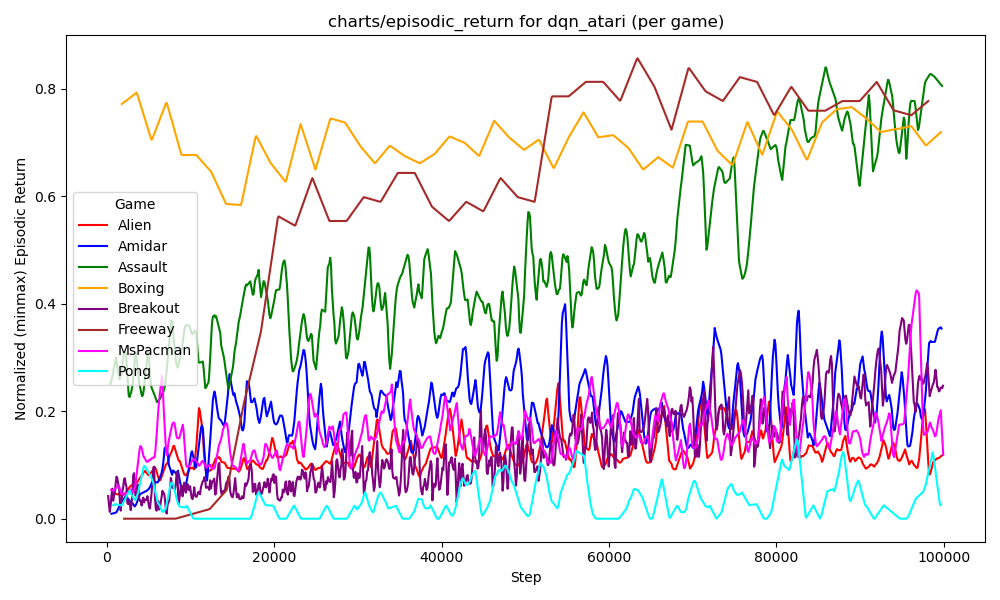
\includegraphics[width=0.6\textwidth]{figures/dqn/charts_episodic_return_per_game_minmax_dqn_atari.png}
	\caption{DQN returns (min--max normalized) by game.}
	\label{fig:dqn_return_pergame_minmax}
\end{figure}

Different environments see dramatically different results: 
\emph{Freeway} often approaches high normalized scores, while 
\emph{Pong} and \emph{MsPacman} remain relatively low 
(especially in the human-normalized scale).

\paragraph{Emissions}
Table~\ref{tab:dqn_emissions} presents the aggregated CO\textsubscript{2}-eq for DQN 
(over all 32 runs). The mean is about \(\textbf{0.00647 kg}\), 
with a minimum of 0.00616 and a maximum near 0.0070.

\begin{table}
	\caption{Carbon emissions (kg\,CO\textsubscript{2}eq) for DQN across 32 runs.}
	\label{tab:dqn_emissions}
	\centering
	\makebox[\textwidth]{%
	\begin{tabularx}{1.1\textwidth}{lXXXXXXXX}
		\toprule
		\textbf{Algorithm} & \textbf{mean} & \textbf{std} & \textbf{median} & 
		\textbf{q25} & \textbf{q75} & \textbf{min} & \textbf{max} & \textbf{iqmean} \\
		\midrule
		DQN & 0.006469 & 0.0002609 & 0.006342 & 0.006296 & 0.006578 & 0.006162 & 0.006997 & 0.006369 \\
		\bottomrule
	\end{tabularx}
	}
\end{table}

\paragraph{Evaluation Results}
Table~\ref{tab:dqn_eval_overall} aggregates final human-/min--max-normalized 
returns \emph{over all 32 runs}. A game-by-game breakdown 
(Table~\ref{tab:dqn_eval_gamewise}) highlights large variability: 
\emph{Freeway} can exceed 0.7 (human norm) or 0.75 (min--max), 
while \emph{Boxing} sees a wide range from $-5$ to nearly $+5$ in human norm.

\begin{table}
	\caption{Overall final evaluation (10 episodes each) for DQN across all runs.}
	\label{tab:dqn_eval_overall}
	\centering
	\begin{tabular}{lcccccccc}
		\toprule
		\textbf{Normalization} & \textbf{mean} & \textbf{std} & \textbf{median} & 
		\textbf{q25} & \textbf{q75} & \textbf{min} & \textbf{max} & \textbf{iqmean} \\
		\midrule
		\textbf{Human} & 0.1353 & 0.7541 & 0.0338 & 0.00072 & 0.398 & -5.024 & 4.738 & 0.1137 \\
		\textbf{Min--Max} & 0.3802 & 0.3099 & 0.2899 & 0.0969 & 0.7143 & 0.0 & 0.9881 & 0.3426 \\
		\bottomrule
	\end{tabular}
\end{table}

\begin{table}
	\caption{Per-game final evaluation for DQN (human- vs.\ min--max normalized). 
		Each cell aggregates 10 episodes $\times$ 4 seeds = 40 total episodes in that game.}
	\label{tab:dqn_eval_gamewise}
	\centering
	\begin{tabular}{llcccc}
		\toprule
		\textbf{Game} & \textbf{Norm} & \textbf{mean} & \textbf{std} & \textbf{min} & \textbf{max}\\
		\midrule
		Alien    & Human   & 0.0624 & 0.0752 & 0.0048 & 0.2636 \\
		    & Min--Max & 0.1607 & 0.1250 & 0.0650 & 0.4950 \\
		\cmidrule{1-6}
		Amidar   & Human   & 0.0226 & 0.0138 & 0.00072 & 0.0450 \\
		   & Min--Max & 0.2005 & 0.1065 & 0.0323 & 0.3733 \\
		\cmidrule{1-6}
		Assault  & Human   & 0.3167 & 0.1120 & -0.0262 & 0.4920 \\
		  & Min--Max & 0.7216 & 0.1703 & 0.2005 & 0.9881 \\
		\cmidrule{1-6}
		Boxing   & Human   & -0.4167 & 1.9504 & -5.0238 & 4.7381 \\
		   & Min--Max & 0.7469 & 0.0635 & 0.5969 & 0.9147 \\
		\cmidrule{1-6}
		Breakout & Human   & 0.3796 & 0.1246 & 0.1096 & 0.6080 \\
		 & Min--Max & 0.3454 & 0.0987 & 0.1316 & 0.5263 \\
		\cmidrule{1-6}
		Freeway  & Human   & 0.7162 & 0.0589 & 0.6419 & 0.8784 \\
		  & Min--Max & 0.7571 & 0.0622 & 0.6786 & 0.9286 \\
		\cmidrule{1-6}
		MsPacman & Human   & 0.0099 & 0.0120 & -0.0076 & 0.0262 \\
		 & Min--Max & 0.1047 & 0.0484 & 0.0340 & 0.1702 \\
		\cmidrule{1-6}
		Pong     & Human   & -0.0083 & 0.0074 & -0.01 & 0.0233 \\
		     & Min--Max & 0.0050 & 0.0221 & 0.0 & 0.1 \\
		\bottomrule
	\end{tabular}
\end{table}

\paragraph{Observations}
In summary:
\begin{itemize}
	\item \textbf{Episodic length} stabilizes around 3500--4000 steps on average, 
	with some extreme runs either terminating quickly or persisting up to 8000 steps.
	\item \textbf{SPS} quickly rises to around 170--180, illustrating the efficiency 
	of the implementation (though some runs are slower).
	\item \textbf{Q-values and TD loss} both exhibit broad variability. On average, 
	Q-values climb steadily to 4--5, but certain runs exceed 10. The TD loss 
	can spike above 3 for some seeds, indicating unstable updates.
	\item \textbf{Returns} show moderate success on easier tasks like \textit{Freeway} 
	and \textit{Boxing}, but remain low in \textit{Pong} or \textit{MsPacman}. Overall, 
	min--max mean is about 0.38, whereas human-normalized is only 0.14 (due in part 
	to highly negative outliers on certain seeds).
	\item \textbf{Emissions} remain modest, at about 0.00647\,kg CO\textsubscript{2}-eq 
	per run. This is unsurprising for a 100k-step setting, but still notable for 
	comparing across algorithms in subsequent sections.
\end{itemize}

DQN thus provides a baseline—relatively simple and lightweight—to which we will 
compare Double DQN, Prioritized Experience Replay, Dueling DQN, and C51 
in the next subsections, evaluating whether each extension justifies 
its additional complexity and energy usage.


\subsubsection{Double DQN}
\label{subsubsec:double_dqn}

\paragraph{(Hyper)Parameters}
Table~\ref{tab:ddqn_hyperparams} shows the main hyperparameters used in our Double DQN implementation.  
As with the baseline DQN (Section~\ref{subsubsec:dqn_baseline}), \texttt{env\_id} and \texttt{seed} vary across the 32 runs (eight Atari games $\times$ four seeds), while the rest remain unchanged. In particular, we again set \texttt{buffer\_size}=10k and \texttt{learning\_starts}=1000. 
The Double DQN update rule differs from standard DQN by separately selecting the action and evaluating its value, aiming to reduce the maximization bias that arises from using the same values to both choose and evaluate an action.

\begin{table}
	\caption{Key hyperparameters for Double DQN. Only \texttt{env\_id} and \texttt{seed} change across runs.}
	\label{tab:ddqn_hyperparams}
	\centering
	\begin{tabular}{ll}
		\toprule
		\textbf{Parameter} & \textbf{Value} \\
		\midrule
		\texttt{exp\_name}                & ddqn\_atari \\
		\texttt{seed}                     & 1..4 \\
		\texttt{torch\_deterministic}     & True \\
		\texttt{cuda}                     & True \\
		\texttt{track}                    & True \\
		\texttt{wandb\_project\_name}     & rlsb \\
		\texttt{capture\_video}           & False \\
		\texttt{save\_model}              & True \\
		\texttt{upload\_model}            & False \\
		\texttt{env\_id}                  & e.g.\ AlienNoFrameskip-v4 \\
		\texttt{total\_timesteps}         & 100000 \\
		\texttt{learning\_rate}           & 0.0001 \\
		\texttt{num\_envs}                & 1 \\
		\texttt{buffer\_size}             & 10000 \\
		\texttt{gamma}                    & 0.99 \\
		\texttt{tau}                      & 1.0 \\
		\texttt{target\_network\_frequency} & 1000 \\
		\texttt{batch\_size}             & 32 \\
		\texttt{start\_e}, \texttt{end\_e} & 1.0 $\to$ 0.01 \\
		\texttt{exploration\_fraction}    & 0.1 \\
		\texttt{learning\_starts}         & 1000 \\
		\texttt{train\_frequency}         & 4 \\
		\bottomrule
	\end{tabular}
\end{table}

\paragraph{Hyperparameter Tuning}
To isolate the effect of Double DQN, we kept all settings identical to the baseline DQN, simply enabling the Double DQN update scheme. 
Following~\cite{van:double_q}, we tested a higher \texttt{target\_network\_frequency} (e.g.\ 3000, scaled from the 10k--20k range in the original paper), but at 100k steps, performance was comparable or slightly better with 1000, so we retained the lower frequency. 

\paragraph{Training Dynamics (Aggregated Over 32 Runs)}
Figure~\ref{fig:ddqn_subfigs} presents key metrics—episodic length, steps per second (SPS), estimated Q-values, and TD loss—aggregated across 32 runs (eight games, four seeds each). 

\begin{figure}
	\centering
	\subfloat[][Episodic length (\texttt{charts\_episodic\_length}). 
	The mean sits around 3500--4000 steps, 
	min--max ranges from near 0 up to 8000.]{
		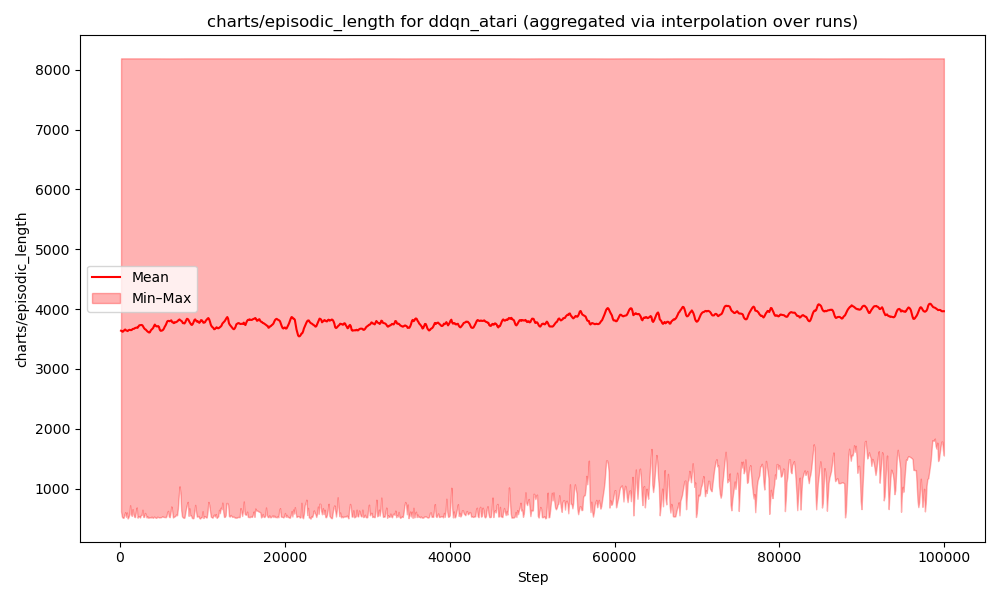
\includegraphics[width=.45\textwidth]{figures/ddqn/charts_episodic_length_ddqn_atari.png}
		\label{fig:ddqn_episodic_length}
	}
	\quad
	\subfloat[][Steps per second (SPS). After an initial climb near 180, 
	the mean gradually settles around 165--170.]{
		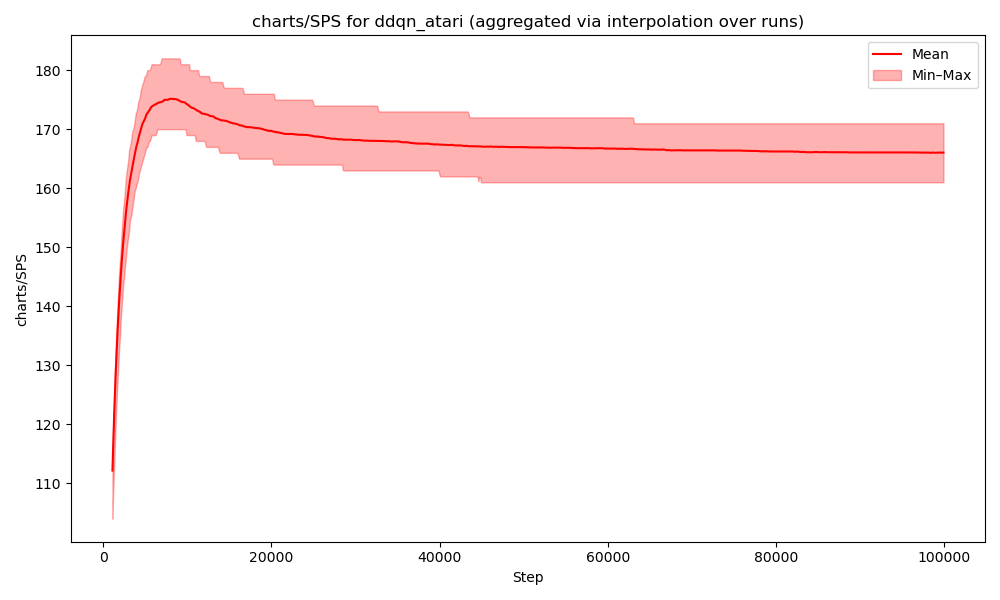
\includegraphics[width=.45\textwidth]{figures/ddqn/charts_SPS_ddqn_atari.png}
		\label{fig:ddqn_sps}
	}
	\\[1em]
	\subfloat[][Estimated Q-values (\texttt{losses/q\_values}). 
	The mean climbs from 0 to about 2--3, 
	with upper outliers above 6.]{
		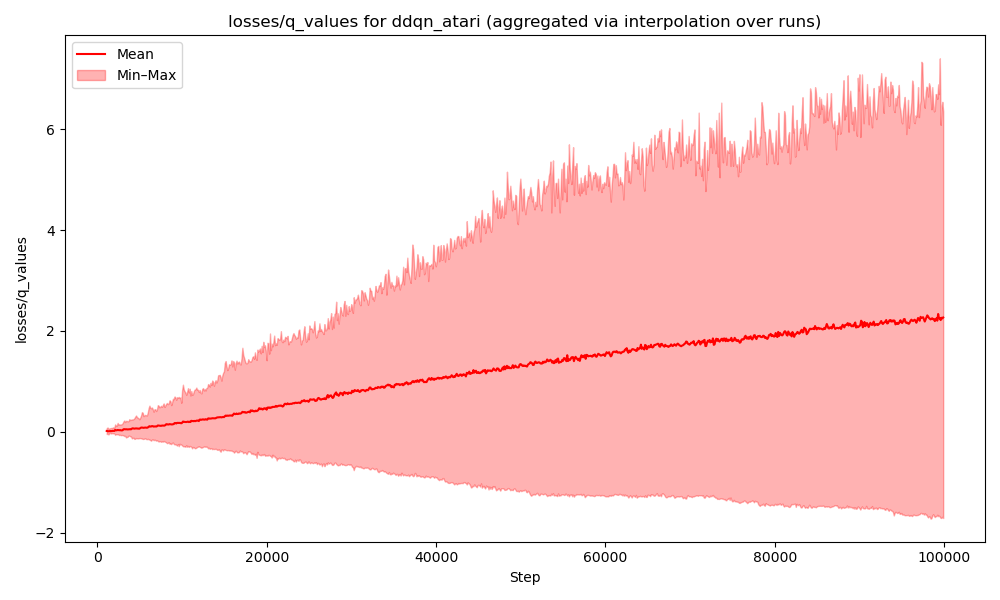
\includegraphics[width=.45\textwidth]{figures/ddqn/losses_q_values_ddqn_atari.png}
		\label{fig:ddqn_q_values}
	}
	\quad
	\subfloat[][TD loss (\texttt{losses/td\_loss}). 
	Occasional spikes above 2.0 reflect instability on certain seeds.]{
		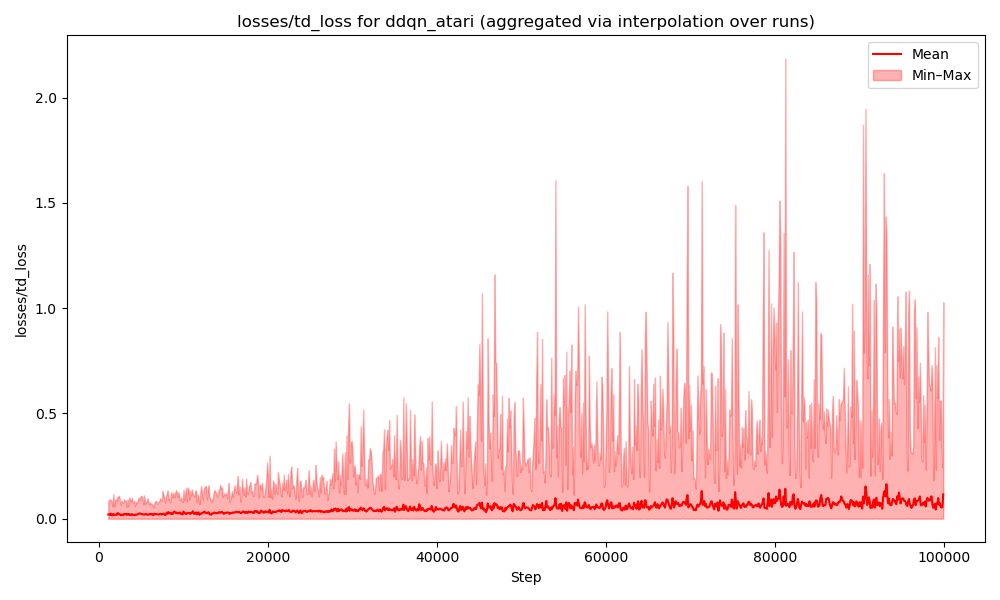
\includegraphics[width=.45\textwidth]{figures/ddqn/losses_td_loss_ddqn_atari.png}
		\label{fig:ddqn_td_loss}
	}
	\caption{Double DQN training metrics over 100k steps, aggregated over 32 runs.}
	\label{fig:ddqn_subfigs}
\end{figure}

Episodic length and SPS curves are very similar to baseline DQN’s (Section~\ref{subsubsec:dqn_baseline}). 
Meanwhile, the mean Q-values grow more modestly than DQN’s (which often exceed 4--5 by the end), suggesting 
Double DQN’s approach does mitigate overestimation somewhat. 
TD loss remains low overall, though some runs spike above 2.0 near late training.

\paragraph{Episodic Return (Human vs.\ Min--Max Normalized)}
Figures~\ref{fig:ddqn_return_human} and \ref{fig:ddqn_return_minmax} show Double DQN’s aggregated episodic returns (human- and min--max-normalized, respectively). 
Figures~\ref{fig:ddqn_return_pergame_human} and \ref{fig:ddqn_return_pergame_minmax} break these results down by game.

\begin{figure}
	\centering
	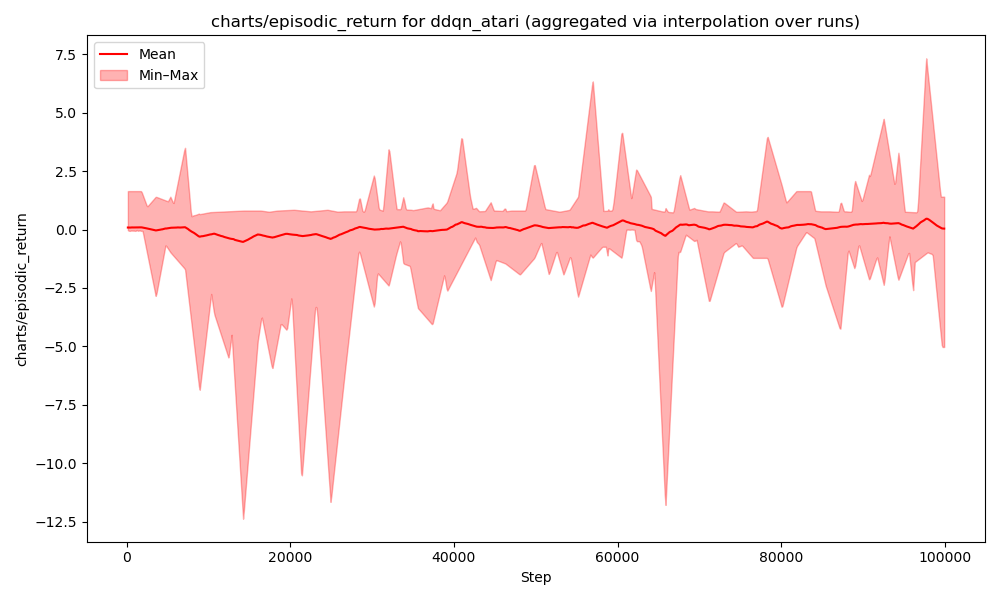
\includegraphics[width=0.6\textwidth]{figures/ddqn/charts_episodic_return_human_ddqn_atari.png}
	\caption{Double DQN episodic return (human-normalized), aggregated across 32 runs.}
	\label{fig:ddqn_return_human}
\end{figure}

\begin{figure}
	\centering
	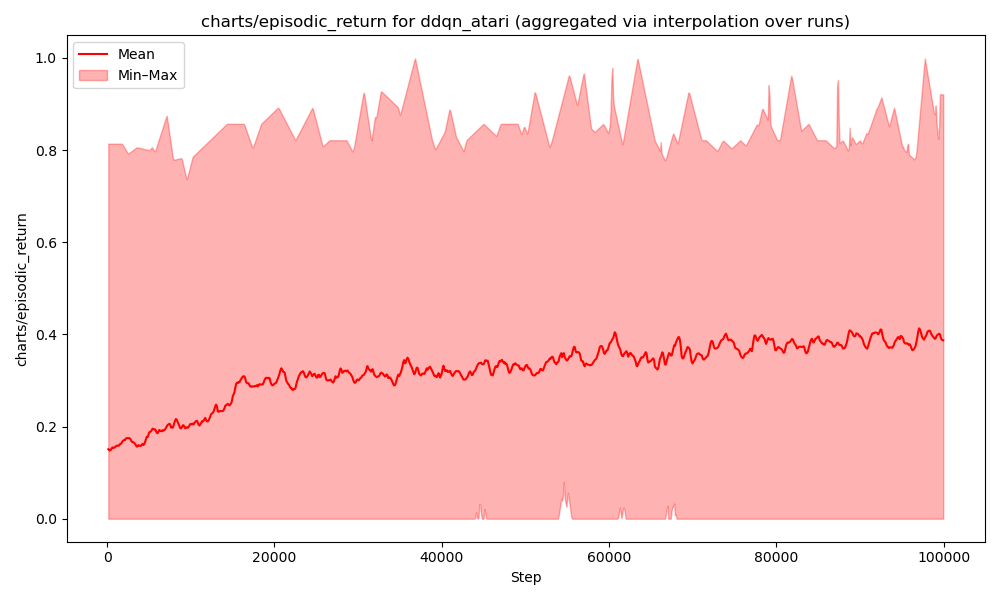
\includegraphics[width=0.6\textwidth]{figures/ddqn/charts_episodic_return_minmax_ddqn_atari.png}
	\caption{Double DQN episodic return (min--max normalized), aggregated across 32 runs.}
	\label{fig:ddqn_return_minmax}
\end{figure}

\begin{figure}
	\centering
	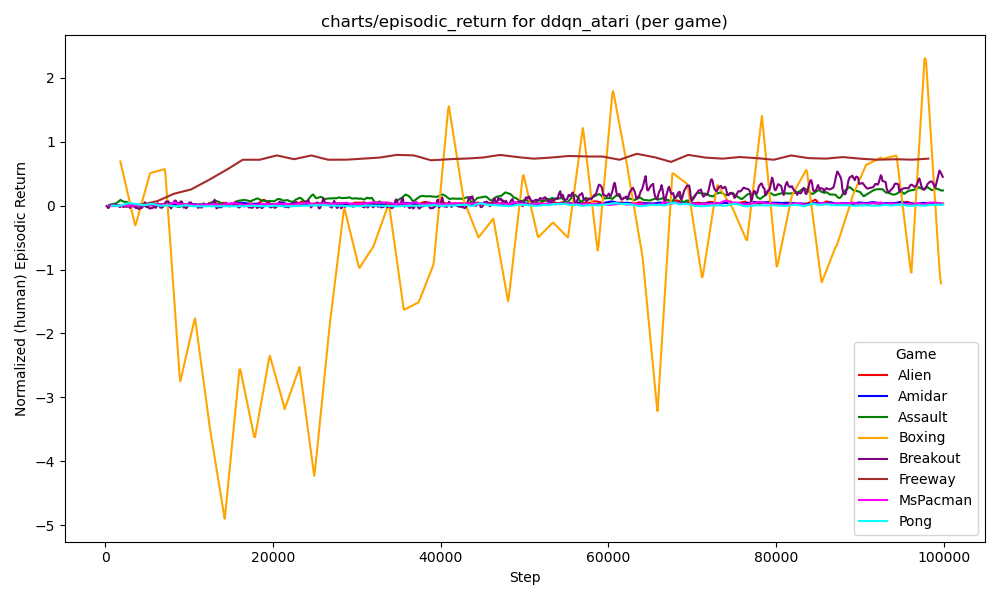
\includegraphics[width=0.6\textwidth]{figures/ddqn/charts_episodic_return_per_game_human_ddqn_atari.png}
	\caption{Double DQN returns per game (human-normalized). 
		Some large negative dips occur in \emph{Boxing}, 
		while \emph{Freeway} remains relatively high.}
	\label{fig:ddqn_return_pergame_human}
\end{figure}

\begin{figure}
	\centering
	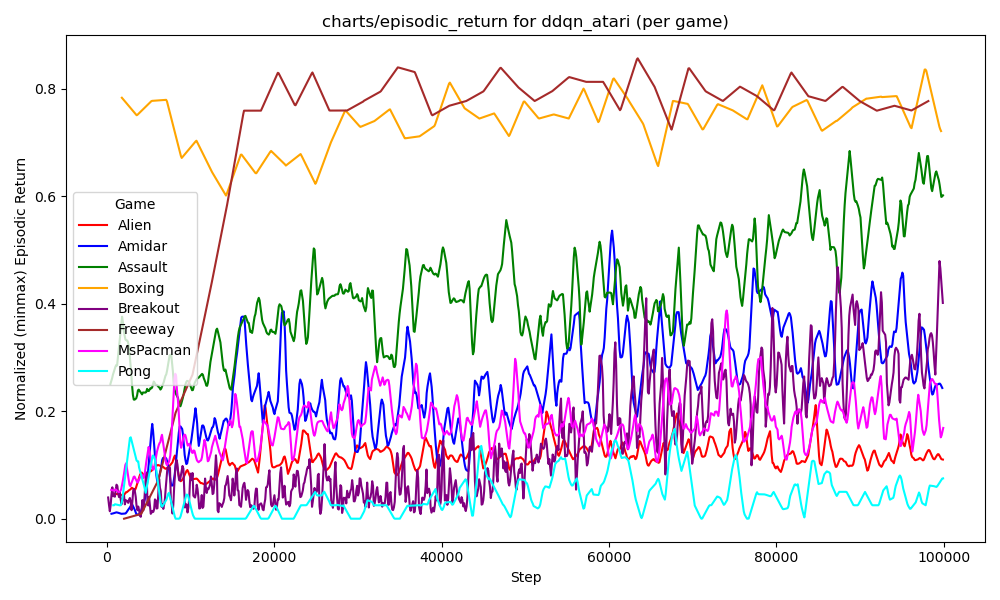
\includegraphics[width=0.6\textwidth]{figures/ddqn/charts_episodic_return_per_game_minmax_ddqn_atari.png}
	\caption{Double DQN returns per game (min--max normalized).}
	\label{fig:ddqn_return_pergame_minmax}
\end{figure}

As in the baseline, \emph{Freeway} can achieve near 0.7--0.8 in human norm, 
while \emph{Boxing} causes occasional highly negative runs. 
Min--max normalized returns rise from $\sim 0.2$ to $\sim 0.4$, 
similar to DQN’s overall trajectory.

\paragraph{Emissions}
Table~\ref{tab:ddqn_emissions} summarizes Double DQN’s CO\textsubscript{2}-eq emissions across 32 runs. 
The mean is about \textbf{0.00667\,kg}, slightly above DQN’s \(\sim 0.00647\).

\begin{table}
	\caption{Carbon emissions (kg\,CO\textsubscript{2}eq) for Double DQN, aggregated over 32 runs.}
	\label{tab:ddqn_emissions}
	\centering
	\makebox[\textwidth]{%
	\begin{tabularx}{1.1\textwidth}{lXXXXXXXX}
		\toprule
		\textbf{Algorithm} & \textbf{mean} & \textbf{std} & \textbf{median} & 
		\textbf{q25} & \textbf{q75} & \textbf{min} & \textbf{max} & \textbf{iqmean} \\
		\midrule
		Double DQN & 0.006672 & 0.000282 & 0.006549 & 0.006477 & 0.006755 
		& 0.006377 & 0.007267 & 0.006565 \\
		\bottomrule
	\end{tabularx}
	}
\end{table}

\paragraph{Evaluation Results}
Table~\ref{tab:ddqn_eval_overall} compiles final returns (human-/min--max normalization) aggregated over the 32 runs. 
Compared to DQN’s \(\sim\!0.135\) (human) and \(\sim\!0.380\) (min--max), Double DQN attains 0.023 (human) and 0.374 (min--max). 
While the min--max average is comparable, the human-normalized mean is noticeably lower due to substantial negative outliers (again, notably \emph{Boxing}).

\begin{table}
	\caption{Overall final evaluation (10 episodes each) for Double DQN across 32 runs.}
	\label{tab:ddqn_eval_overall}
	\centering
	\makebox[\textwidth]{%
	\begin{tabularx}{1.1\textwidth}{lXXXXXXXX}
		\toprule
		\textbf{Normalization} & \textbf{mean} & \textbf{std} & \textbf{median} & 
		\textbf{q25} & \textbf{q75} & \textbf{min} & \textbf{max} & \textbf{iqmean} \\
		\midrule
		\textbf{Human} & 0.0226 & 1.0083 & 0.0527 & 0.0127 & 0.2871 & -8.5952 & 2.5952 & 0.0894 \\
		\textbf{Min--Max} & 0.3737 & 0.2854 & 0.2887 & 0.1244 & 0.7054 & 0.0 & 1.0 & 0.3272 \\
		\bottomrule
	\end{tabularx}
	}
\end{table}

Table~\ref{tab:ddqn_eval_gamewise} shows the game-by-game breakdown, indicating \emph{Boxing} yields a min of -8.5952 and max of 2.5952 in human-normalized scale, dragging down the overall mean. Meanwhile, \emph{Freeway} remains consistently high.

\begin{table}
	\caption{Per-game final evaluation for Double DQN (human- vs.\ min--max normalized). 
		Each row aggregates 40 total episodes (10 per seed).}
	\label{tab:ddqn_eval_gamewise}
	\centering
	\begin{tabular}{llcccc}
		\toprule
		\textbf{Game} & \textbf{Norm} & \textbf{mean} & \textbf{std} & \textbf{min} & \textbf{max}\\
		\midrule
		Alien    & Human   & 0.0514 & 0.0340 & 0.0094 & 0.1327 \\
		& Min--Max & 0.1424 & 0.0565 & 0.0725 & 0.2775 \\
		\cmidrule{1-6}
		Amidar   & Human   & 0.0320 & 0.0222 & 0.0127 & 0.0953 \\
		& Min--Max & 0.2729 & 0.1708 & 0.1244 & 0.7604 \\
		\cmidrule{1-6}
		Assault  & Human   & 0.2310 & 0.1071 & -0.0427 & 0.4103 \\
		& Min--Max & 0.5913 & 0.1628 & 0.1754 & 0.8640 \\
		\cmidrule{1-6}
		Boxing   & Human   & -1.1607 & 2.4963 & -8.5952 & 2.5952 \\
		& Min--Max & 0.7227 & 0.0813 & 0.4806 & 0.8450 \\
		\cmidrule{1-6}
		Breakout & Human   & 0.2666 & 0.1470 & 0.0764 & 0.8738 \\
		& Min--Max & 0.2559 & 0.1165 & 0.1053 & 0.7368 \\
		\cmidrule{1-6}
		Freeway  & Human   & 0.7213 & 0.0493 & 0.6419 & 0.8784 \\
		& Min--Max & 0.7625 & 0.0521 & 0.6786 & 0.9286 \\
		\cmidrule{1-6}
		MsPacman & Human   & 0.0291 & 0.0245 & -0.0037 & 0.0730 \\
		& Min--Max & 0.1820 & 0.0986 & 0.0497 & 0.3586 \\
		\cmidrule{1-6}
		Pong     & Human   & 0.0100 & 0.0559 & -0.01 & 0.3233 \\
		& Min--Max & 0.0600 & 0.1676 & 0.0   & 1.0 \\
		\bottomrule
	\end{tabular}
\end{table}

\paragraph{Comparison with Baseline DQN}
Beyond the final statistics, we can compare Q-values and TD loss directly via overlapping curves. Figure~\vref{fig:dqn_vs_ddqn_qvalues} shows the \texttt{losses/q\_values} for both algorithms, with \texttt{ddqn\_atari} in red and \texttt{dqn\_atari} in gold; Double DQN’s mean Q-values grow more slowly, suggesting less overestimation. Figure~\ref{fig:dqn_vs_ddqn_td_loss} indicates TD loss remains similarly small for both, though DQN occasionally spikes higher. The barplot in figure~\ref{fig:emissions_dqn_ddqn} shows the mean emissions side-by-side.

\begin{figure}
	\centering
	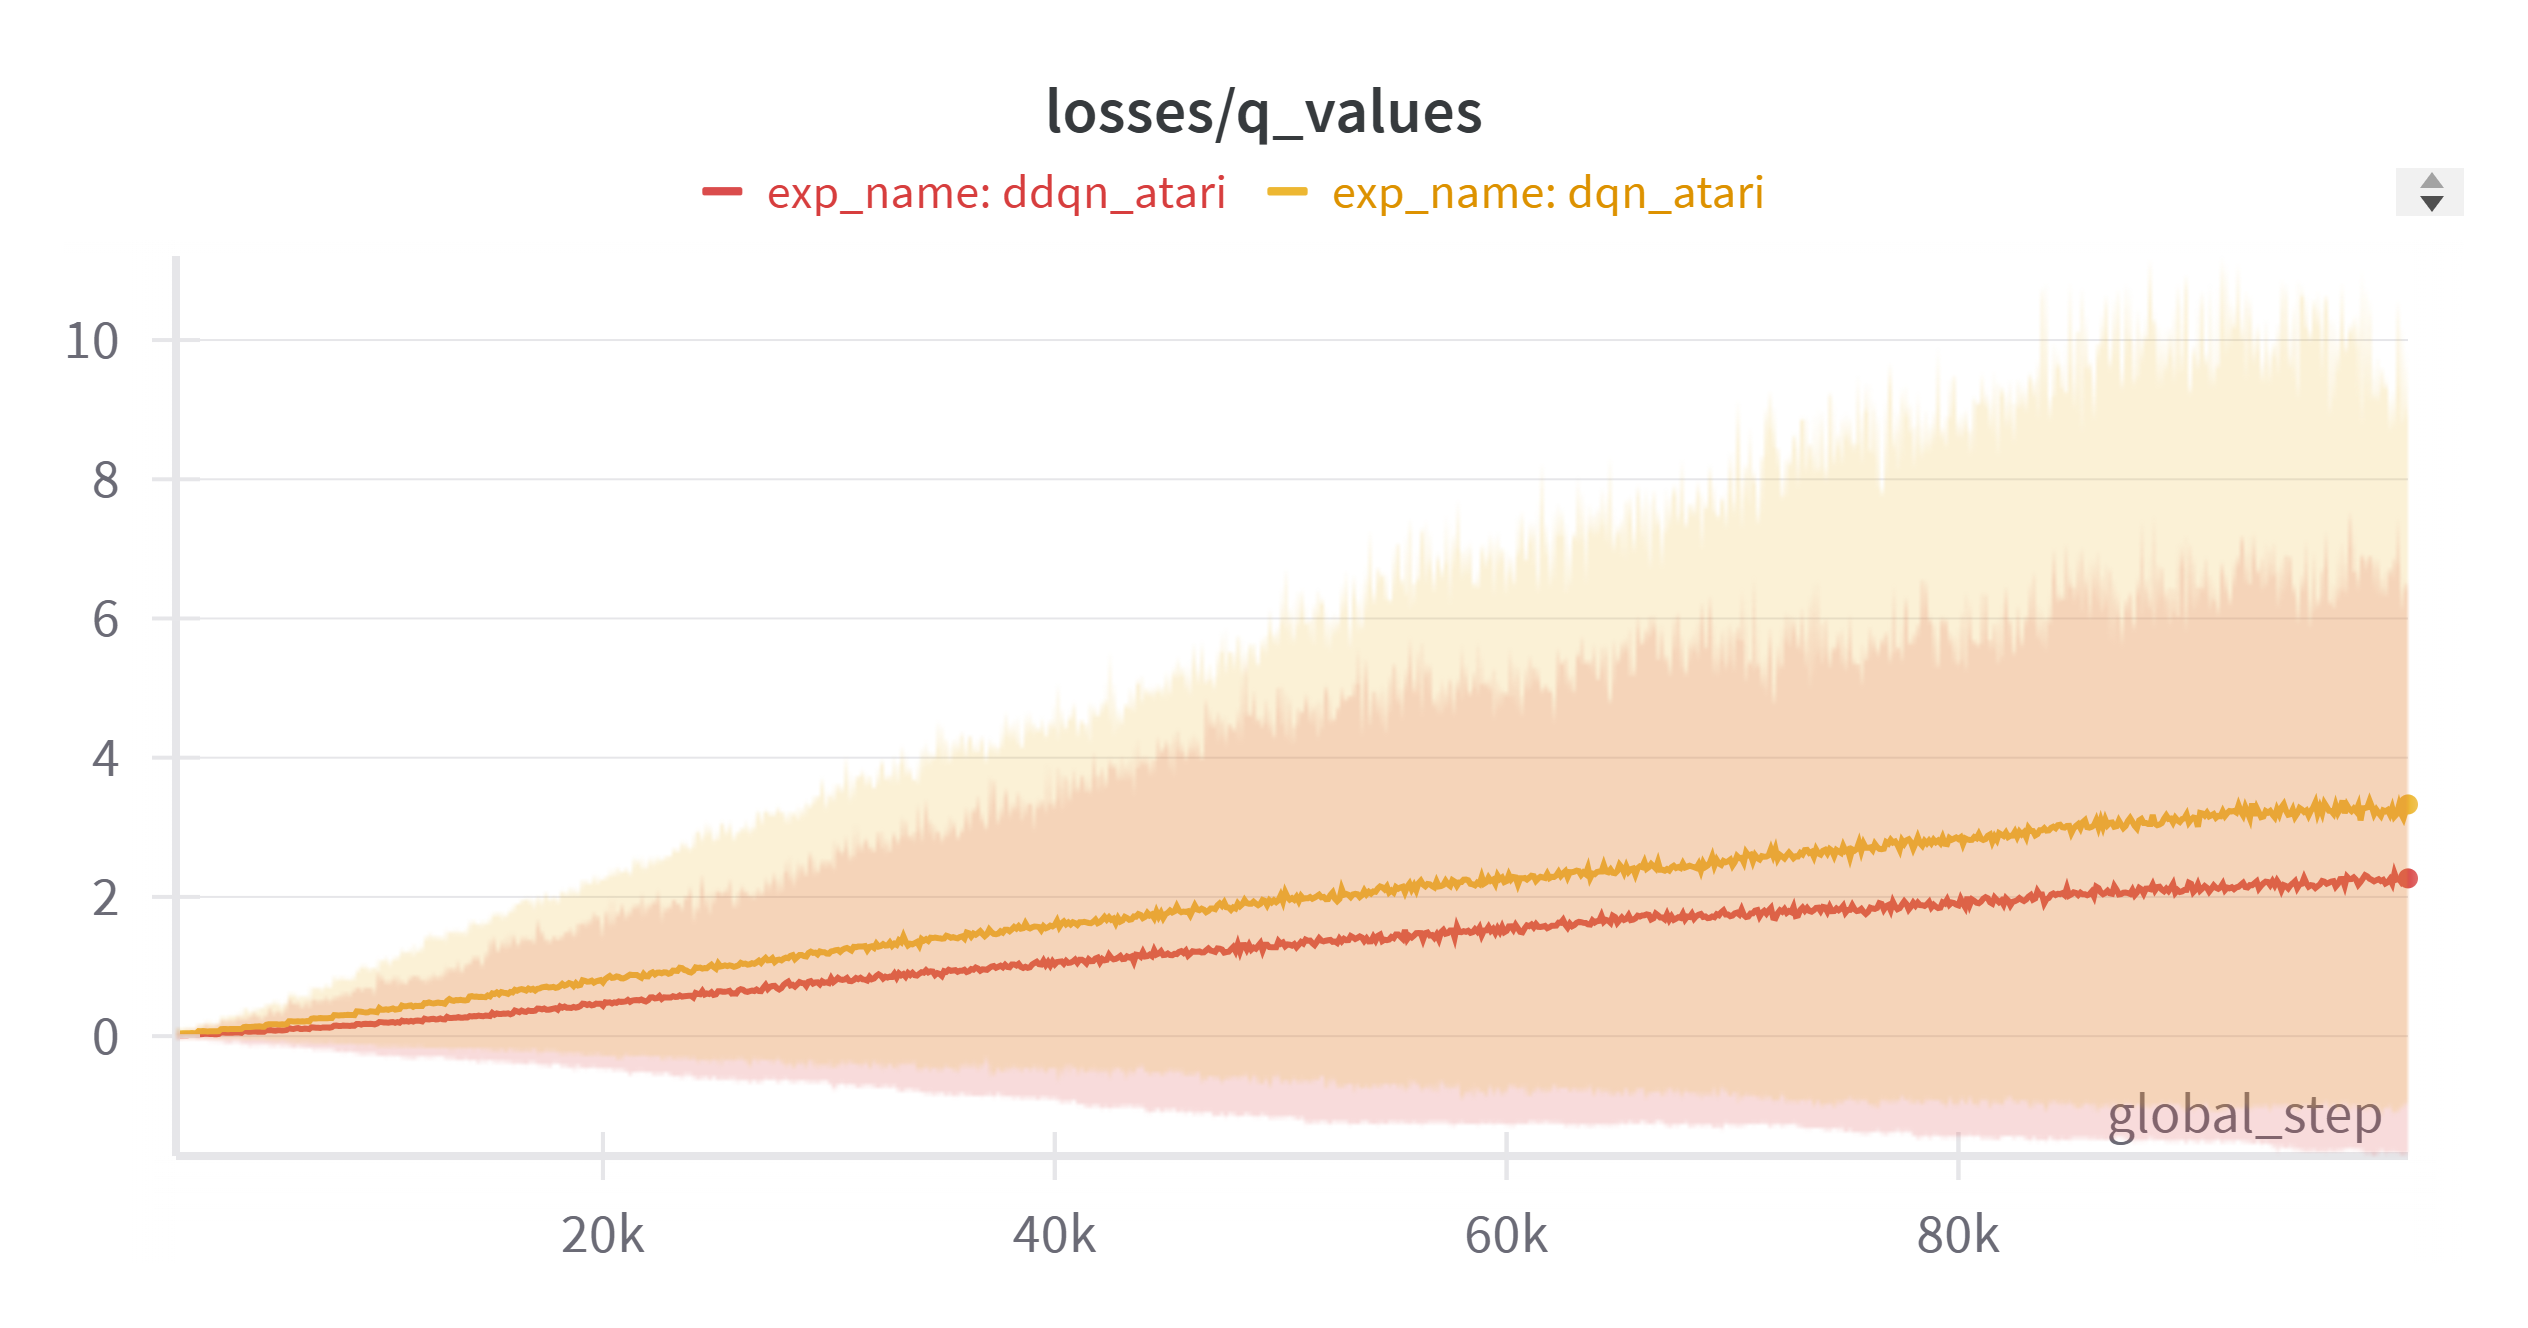
\includegraphics[width=0.6\textwidth]{figures/ddqn/comparison_losses_q_values_dqn_ddqn.png}
	\caption{Comparison of mean Q-values (with min--max shading) for DQN (gold) vs.\ Double DQN (red).}
	\label{fig:dqn_vs_ddqn_qvalues}
\end{figure}

\begin{figure}
	\centering
	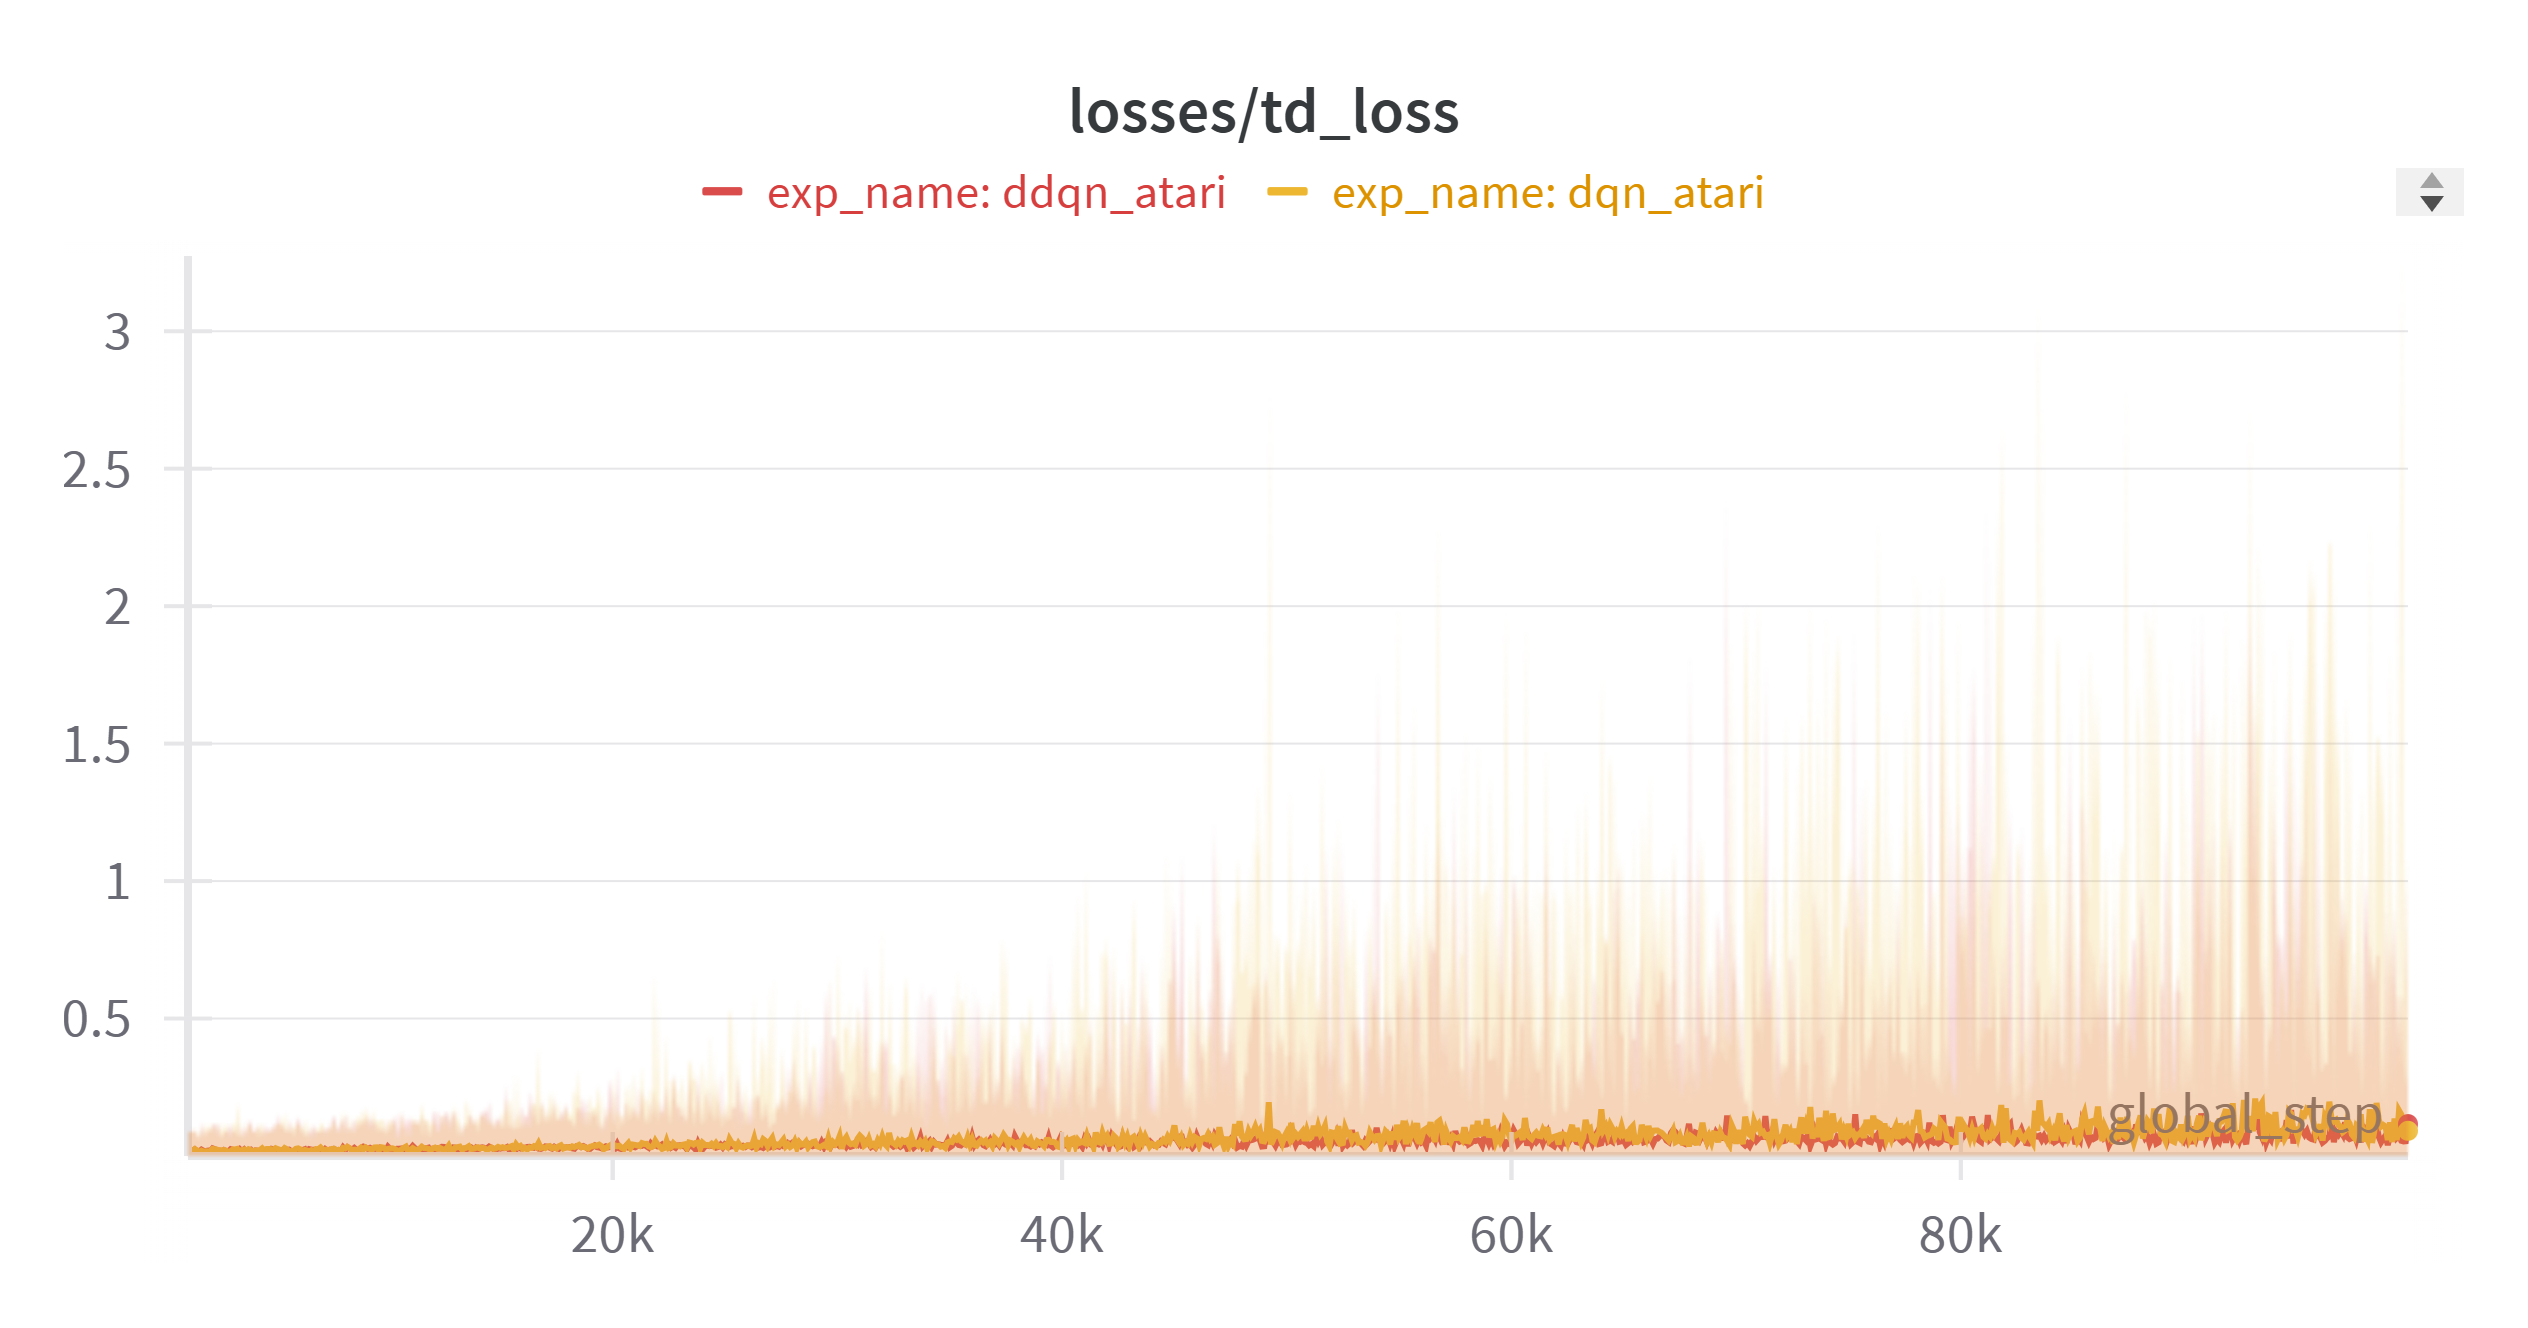
\includegraphics[width=0.6\textwidth]{figures/ddqn/comparison_losses_td_loss_dqn_ddqn.png}
	\caption{Comparison of TD loss for DQN (gold) vs.\ Double DQN (red). 
		Both remain near 0 for extended periods, though DQN shows slightly higher spikes.}
	\label{fig:dqn_vs_ddqn_td_loss}
\end{figure}


\begin{figure}
	\centering
	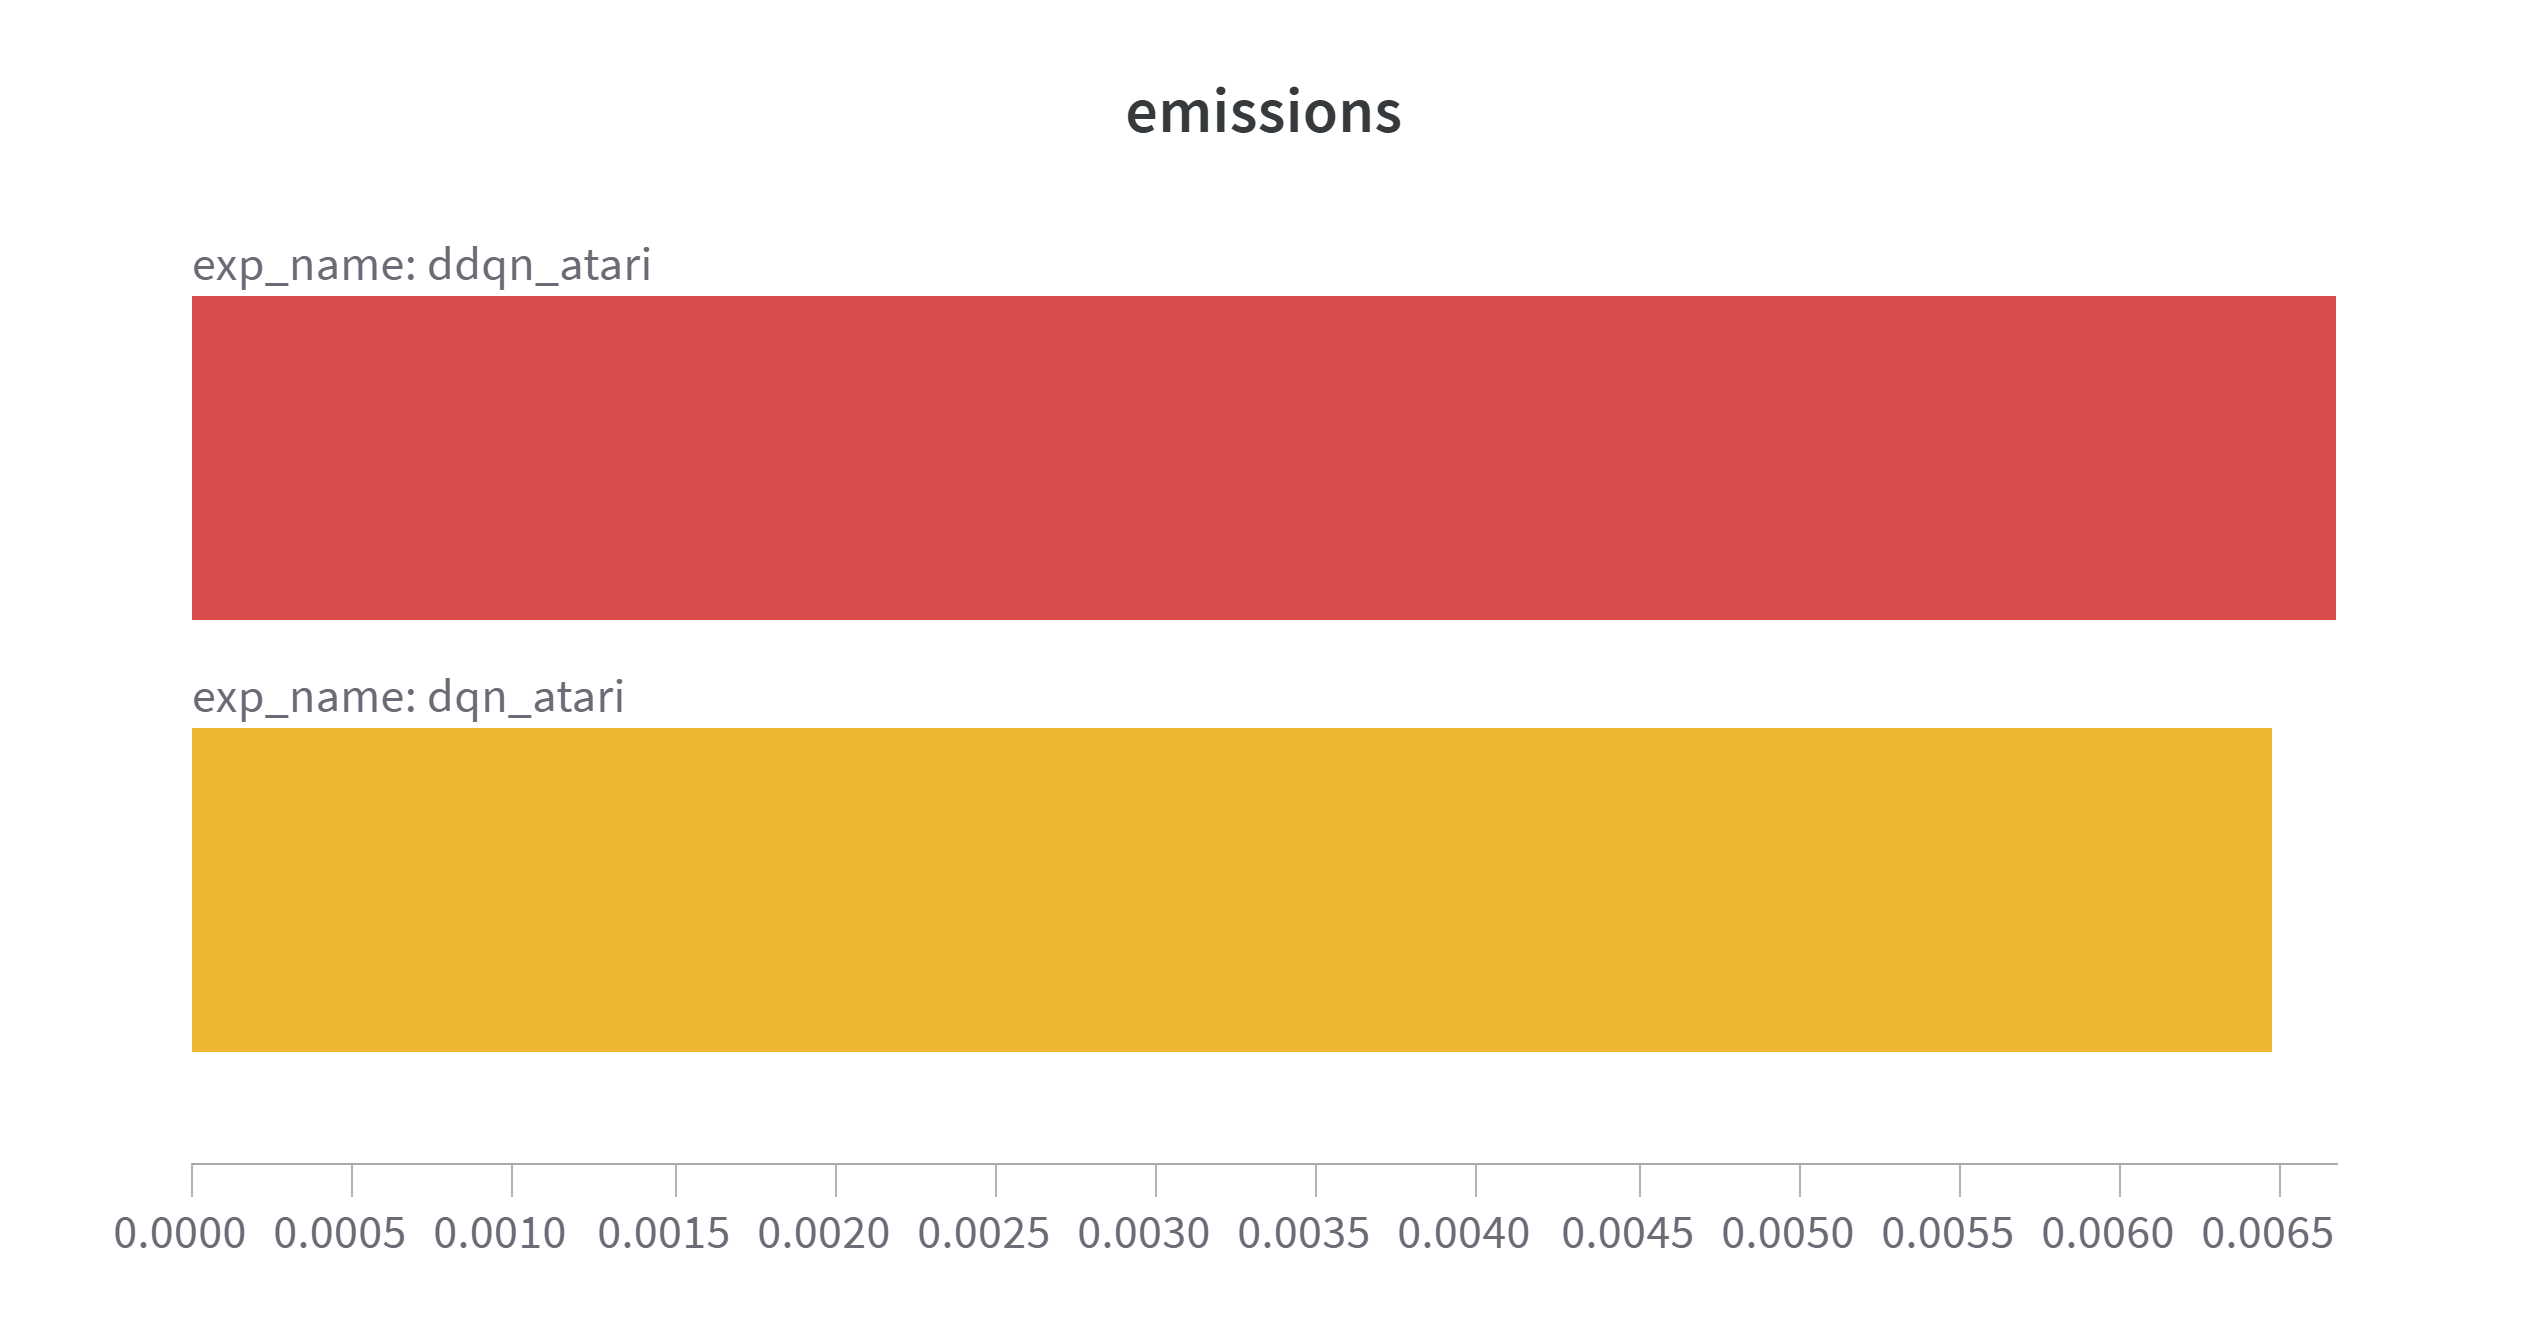
\includegraphics[width=0.6\textwidth]{figures/ddqn/emissions_dqn_ddqn.png}
	\caption{Mean emissions of DQN (gold) and Double DQN (red).}
	\label{fig:emissions_dqn_ddqn}
\end{figure}

Overall, Double DQN indeed moderates Q-value inflation compared to standard DQN, 
but under the 100k-step constraint, this reduction in overestimation does not strongly translate 
into consistently higher final returns.

\paragraph{Observations}
\begin{itemize}
	\item \textbf{Q-values and Losses:} Double DQN’s Q-values peak lower than DQN’s (about 2--3 vs.\ 4--5), aligning with the bias-reduction theory. TD losses remain small for both algorithms, with occasional spikes.
	\item \textbf{Performance:} The min--max normalized mean (0.374) is nearly the same as DQN’s (0.380), while human-normalized is actually lower (0.023 vs.\ 0.135) due to certain highly negative runs, especially in \emph{Boxing}.
	\item \textbf{Emissions:} Average $\sim0.00667$\,kg CO\textsubscript{2}-eq, slightly higher than DQN’s $0.00647$\,kg.
\end{itemize}

Hence, although Double DQN successfully limits Q-value overestimation, its advantage does not 
fully manifest in higher aggregate returns at 100k steps—indicating that more extensive training 
or additional refinements may be needed to reap its potential performance gains.


\subsubsection{Prioritized Experience Replay}
\label{subsubsec:per}

\paragraph{(Hyper)Parameters}

\begin{table}
	\caption{Key hyperparameters for Prioritized Experience Replay (PER). Only \texttt{env\_id} and \texttt{seed} vary across runs.}
	\label{tab:per_hyperparams}
	\centering
	\begin{tabular}{ll}
		\toprule
		\textbf{Parameter} & \textbf{Value} \\
		\midrule
		\texttt{exp\_name}                & per\_atari \\
		\texttt{seed}                     & 1..4 \\
		\texttt{torch\_deterministic}     & True \\
		\texttt{cuda}                     & True \\
		\texttt{track}                    & True \\
		\texttt{wandb\_project\_name}     & rlsb \\
		\texttt{capture\_video}           & False \\
		\texttt{save\_model}              & True \\
		\texttt{upload\_model}            & False \\
		\texttt{env\_id}                  & e.g.\ AmidarNoFrameskip-v4 \\
		\texttt{total\_timesteps}         & 100000 \\
		\texttt{learning\_rate}           & 0.0001 \\
		\texttt{num\_envs}                & 1 \\
		\texttt{buffer\_size}             & 10000 \\
		\texttt{gamma}                    & 0.99 \\
		\texttt{tau}                      & 1.0 \\
		\texttt{target\_network\_frequency} & 1000 \\
		\texttt{batch\_size}             & 32 \\
		\texttt{start\_e}, \texttt{end\_e} & 1.0 $\to$ 0.01 \\
		\texttt{exploration\_fraction}    & 0.1 \\
		\texttt{learning\_starts}         & 1000 \\
		\texttt{train\_frequency}         & 4 \\
		\bottomrule
	\end{tabular}
\end{table}

\paragraph{Hyperparameter Tuning}
We retained the same settings as baseline DQN (Section~\ref{subsubsec:dqn_baseline}) to highlight PER’s impact alone. Although \cite{schaul:prioritized} suggests lowering the learning rate by a factor of four, our tests at 100k steps showed $1\times10^{-4}$ worked better. Figure~\ref{fig:per_lr_comparison} compares these rates on \emph{Breakout}, indicating faster convergence at $1\times10^{-4}$.  

We also explored two implementations of the PER replay buffer—a \texttt{numpy}-based priority queue (for consistency) and a \texttt{torch}-based version. The \texttt{numpy} approach proved much slower, so we used the \texttt{torch} buffer in the final runs. Although the other DQN variants employ somewhat different replay optimizations (some from Stable Baselines), these differences did not appear to invalidate direct comparisons.

\begin{figure}
	\centering
	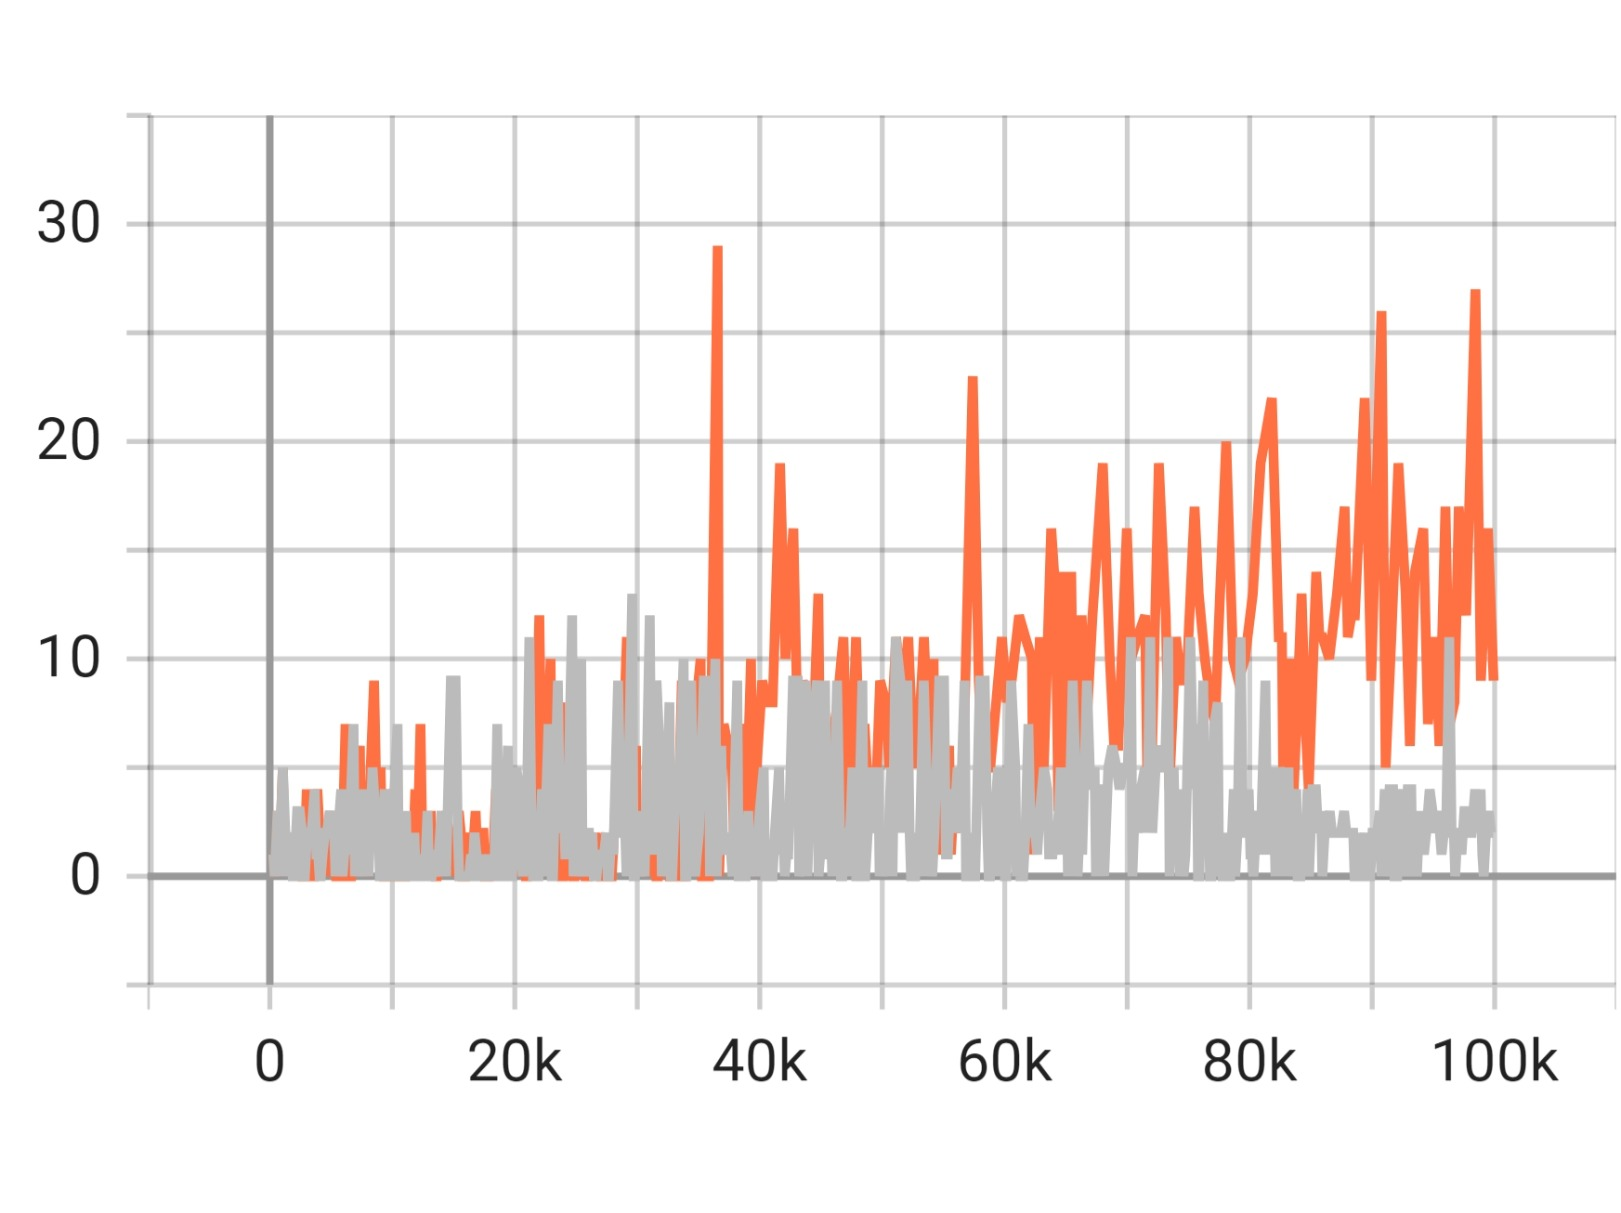
\includegraphics[width=0.55\textwidth]{figures/per/per_lr_charts_episodic_return.jpeg}
	\caption{Comparison of learning rates for PER on \emph{Breakout}. 
		Orange curve: $1\times10^{-4}$ (our final choice). 
		Gray curve: $\tfrac{1}{4}\times10^{-4}$ (as per \cite{schaul:prioritized}).}
	\label{fig:per_lr_comparison}
\end{figure}

\paragraph{Training Dynamics}
Figure~\ref{fig:per_training_metrics} aggregates four key metrics (episodic length, steps per second, Q-values, and TD loss) over 32 runs (eight games, four seeds each):

\begin{figure}
	\centering
	\subfloat[][Episodic length (\texttt{charts\_episodic\_length}). 
	The mean hovers around 3500--4000, and min--max runs from near 0 up to 8000.]{
		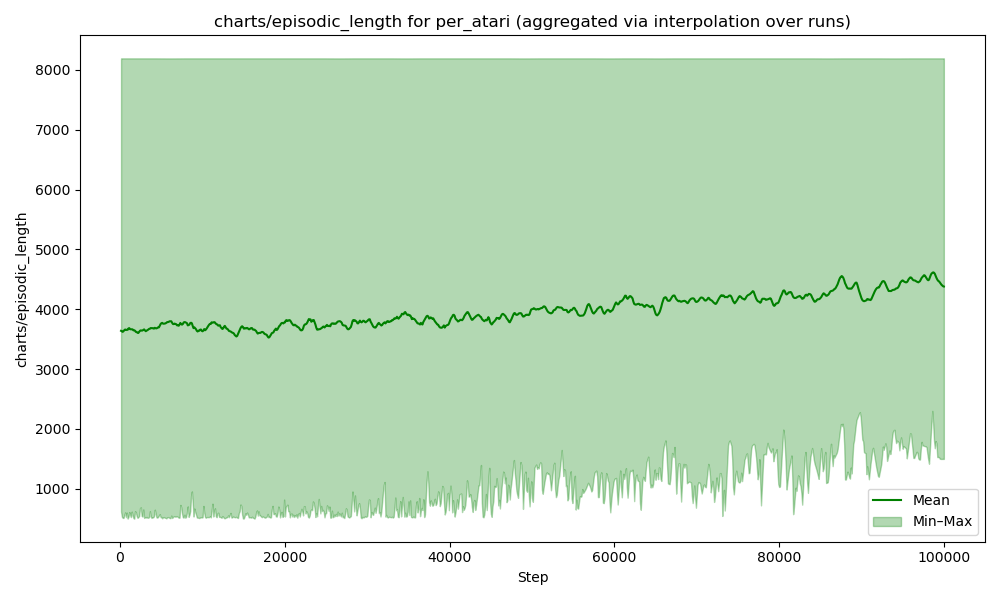
\includegraphics[width=.45\textwidth]{figures/per/charts_episodic_length_per_atari.png}
		\label{fig:per_episodic_length}
	}
	\quad
	\subfloat[][Steps per second (SPS). 
	The mean peaks above 170, then gradually declines to ~150--160.]{
		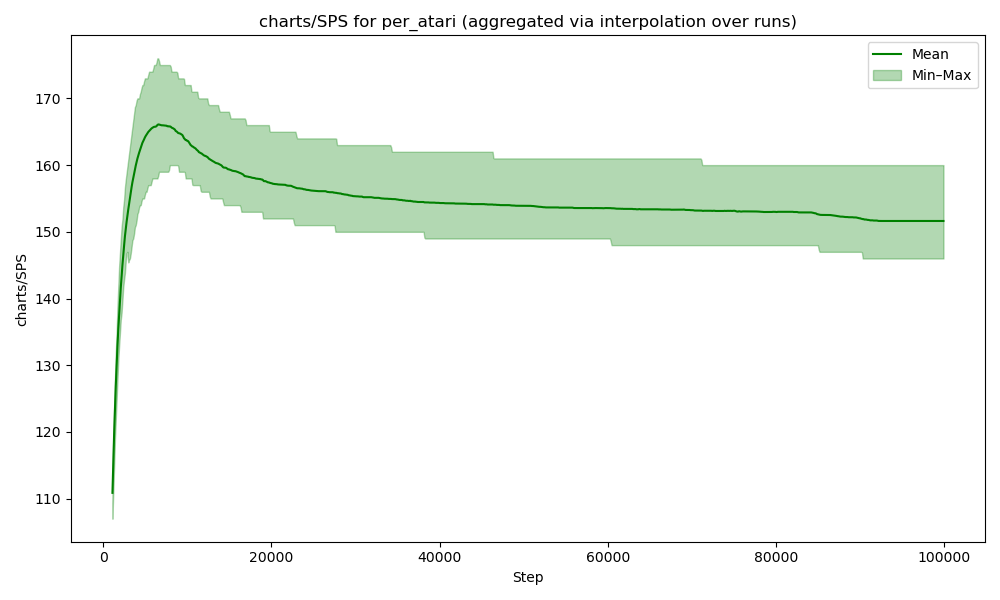
\includegraphics[width=.45\textwidth]{figures/per/charts_SPS_per_atari.png}
		\label{fig:per_sps}
	}
	\\[1em]
	\subfloat[][Q-values (\texttt{losses/q\_values}). 
	The mean eventually surpasses 4--5, with outliers above 14.]{
		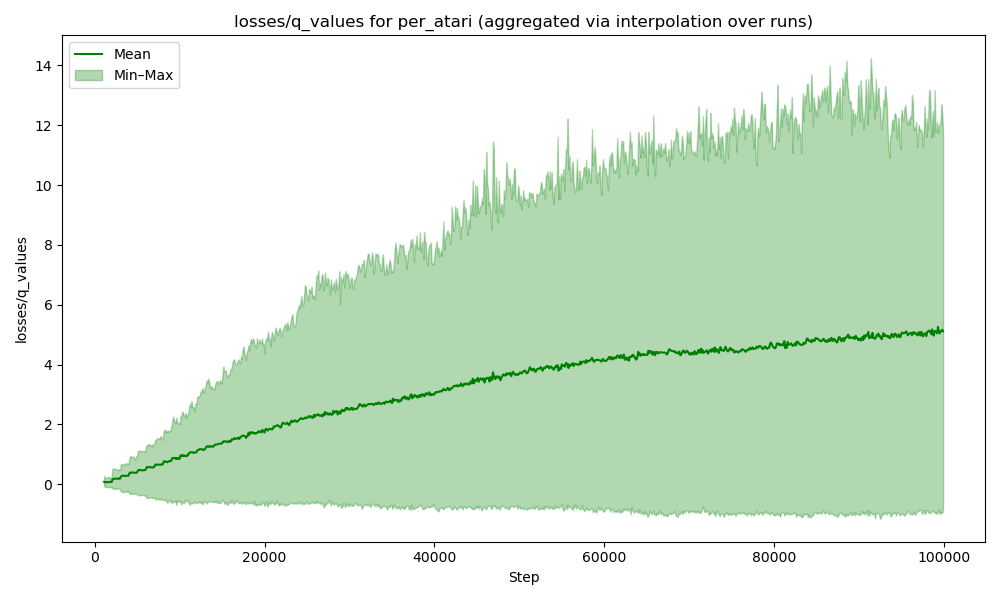
\includegraphics[width=.45\textwidth]{figures/per/losses_q_values_per_atari.png}
		\label{fig:per_q_values}
	}
	\quad
	\subfloat[][TD loss (\texttt{losses/td\_loss}). 
	Some runs spike above 3--4, showing instability in late training.]{
		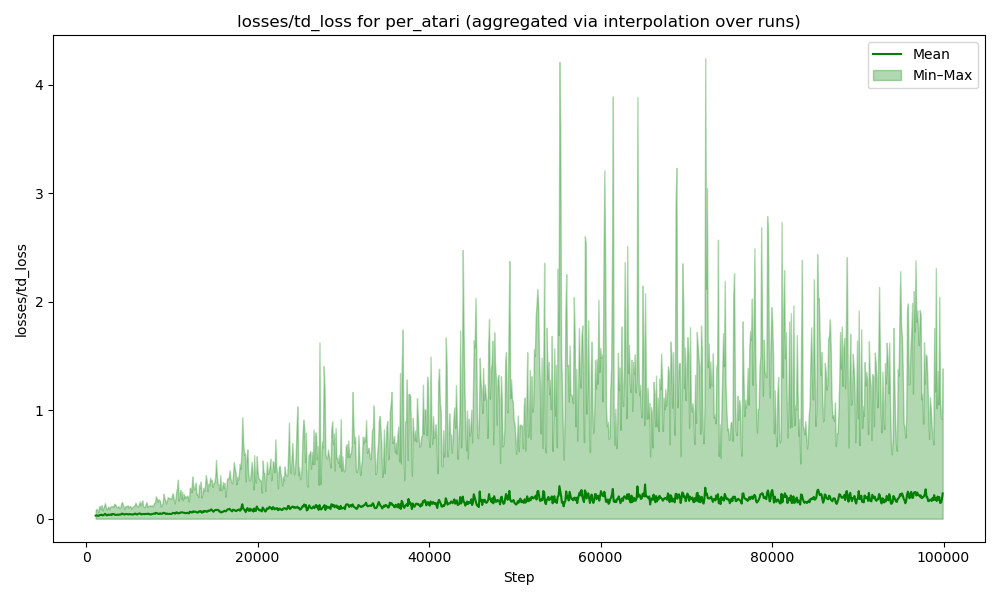
\includegraphics[width=.45\textwidth]{figures/per/losses_td_loss_per_atari.png}
		\label{fig:per_td_loss}
	}
	\caption{PER training metrics over 100k steps, interpolated across 32 runs.}
	\label{fig:per_training_metrics}
\end{figure}

PER shows Q-values approaching or exceeding those of baseline DQN (which typically topped at 4--5). The TD loss is small on average but spikes in certain runs, suggesting that prioritizing high-error samples can exacerbate updates in some episodes.

\paragraph{Episodic Return (Aggregated)}
Figures~\ref{fig:per_return_human} (human-normalized) and \ref{fig:per_return_minmax} (min--max) show PER’s aggregated episodic returns. The mean in human-normalized scale oscillates around zero, occasionally dipping below $-2$ or $-3$ in some seeds.

\begin{figure}
	\centering
	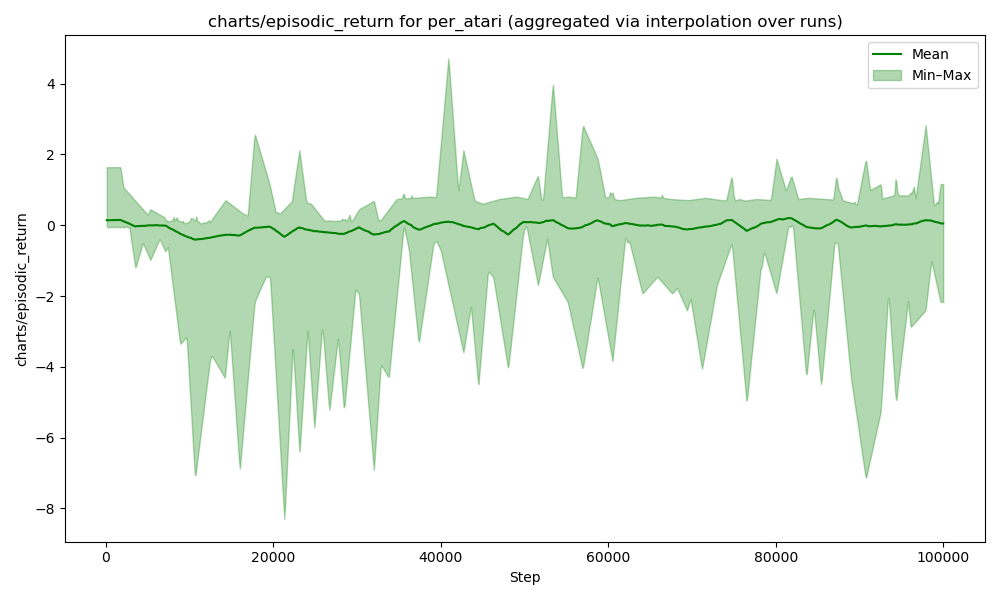
\includegraphics[width=0.6\textwidth]{figures/per/charts_episodic_return_human_per_atari.png}
	\caption{PER episodic return (human-normalized), aggregated over 32 runs. 
		Negative outliers appear for certain seeds/environments.}
	\label{fig:per_return_human}
\end{figure}

\begin{figure}
	\centering
	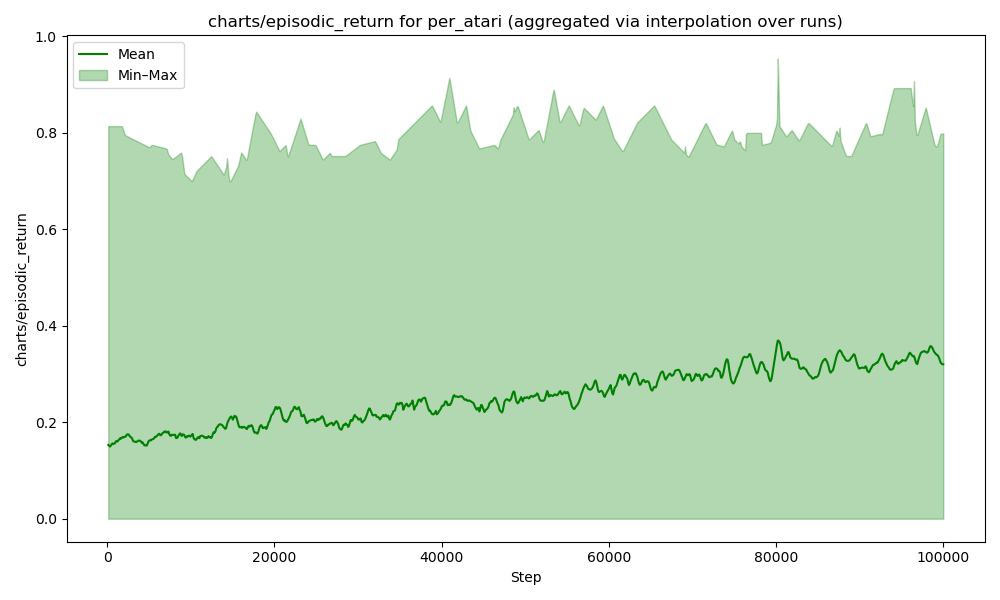
\includegraphics[width=0.6\textwidth]{figures/per/charts_episodic_return_minmax_per_atari.png}
	\caption{PER episodic return (min--max normalized), aggregated over 32 runs.}
	\label{fig:per_return_minmax}
\end{figure}

\paragraph{Per-Game Returns}
Figures~\ref{fig:per_return_pergame_human} and \ref{fig:per_return_pergame_minmax} break down the performance by each Atari game (human vs. min--max normalization). We see, for instance, \emph{Freeway} (orange line in min--max) steadily climbing to around 0.7--0.8, while \emph{Alien} can drop below $-3$ in human scale. 

\begin{figure}
	\centering
	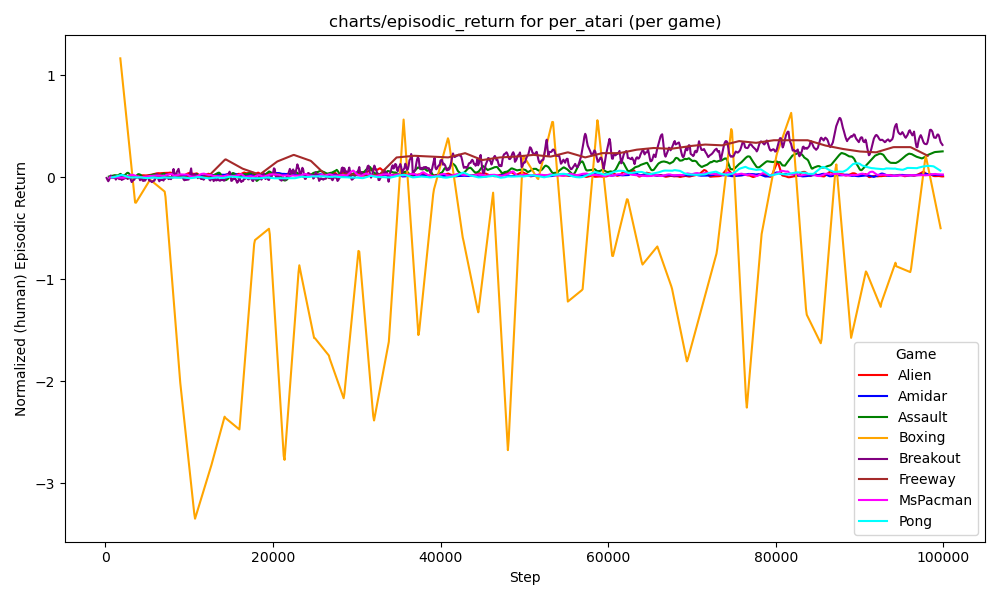
\includegraphics[width=0.6\textwidth]{figures/per/charts_episodic_return_per_game_human_per_atari.png}
	\caption{PER returns per game (human-normalized). 
		\emph{Alien} (orange) exhibits deep negative dips, 
		while \emph{Freeway}, \emph{Assault}, and \emph{Breakout} stay near or above zero.}
	\label{fig:per_return_pergame_human}
\end{figure}

\begin{figure}
	\centering
	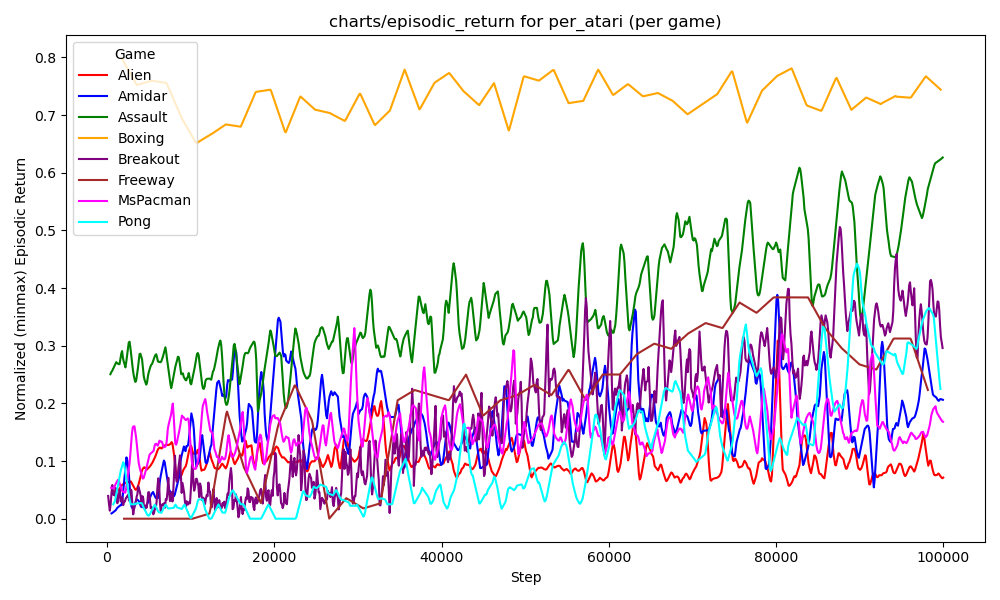
\includegraphics[width=0.6\textwidth]{figures/per/charts_episodic_return_per_game_minmax_per_atari.png}
	\caption{PER returns per game (min--max normalized). 
		\emph{Freeway} (gold line) and \emph{Assault} (green) reach 0.7--0.8 near 100k steps.}
	\label{fig:per_return_pergame_minmax}
\end{figure}

\paragraph{Emissions.}

\begin{table}
	\caption{Carbon emissions (kg\,CO\textsubscript{2}eq) for PER across 32 runs.}
	\label{tab:per_emissions}
	\centering
	\makebox[\textwidth]{%
	\begin{tabularx}{1.1\textwidth}{lXXXXXXXX}
		\toprule
		\textbf{Algorithm} & \textbf{mean} & \textbf{std} & \textbf{median} & \textbf{q25} & \textbf{q75} & \textbf{min} & \textbf{max} & \textbf{iqmean} \\
		\midrule
		PER & 0.007254 & 0.000263 & 0.007146 & 0.007074 & 0.007354 & 0.006935 & 0.007819 & 0.007157 \\
		\bottomrule
	\end{tabularx}
	}
\end{table}

Figure~\ref{fig:per_vs_dqn_emissions} shows a barplot comparing PER’s mean emissions (\(\approx 0.00725\,\mathrm{kg}\)) to DQN’s (\(\approx0.00647\,\mathrm{kg}\)). The overhead of prioritized sampling may partly account for this higher footprint.

\begin{figure}
	\centering
	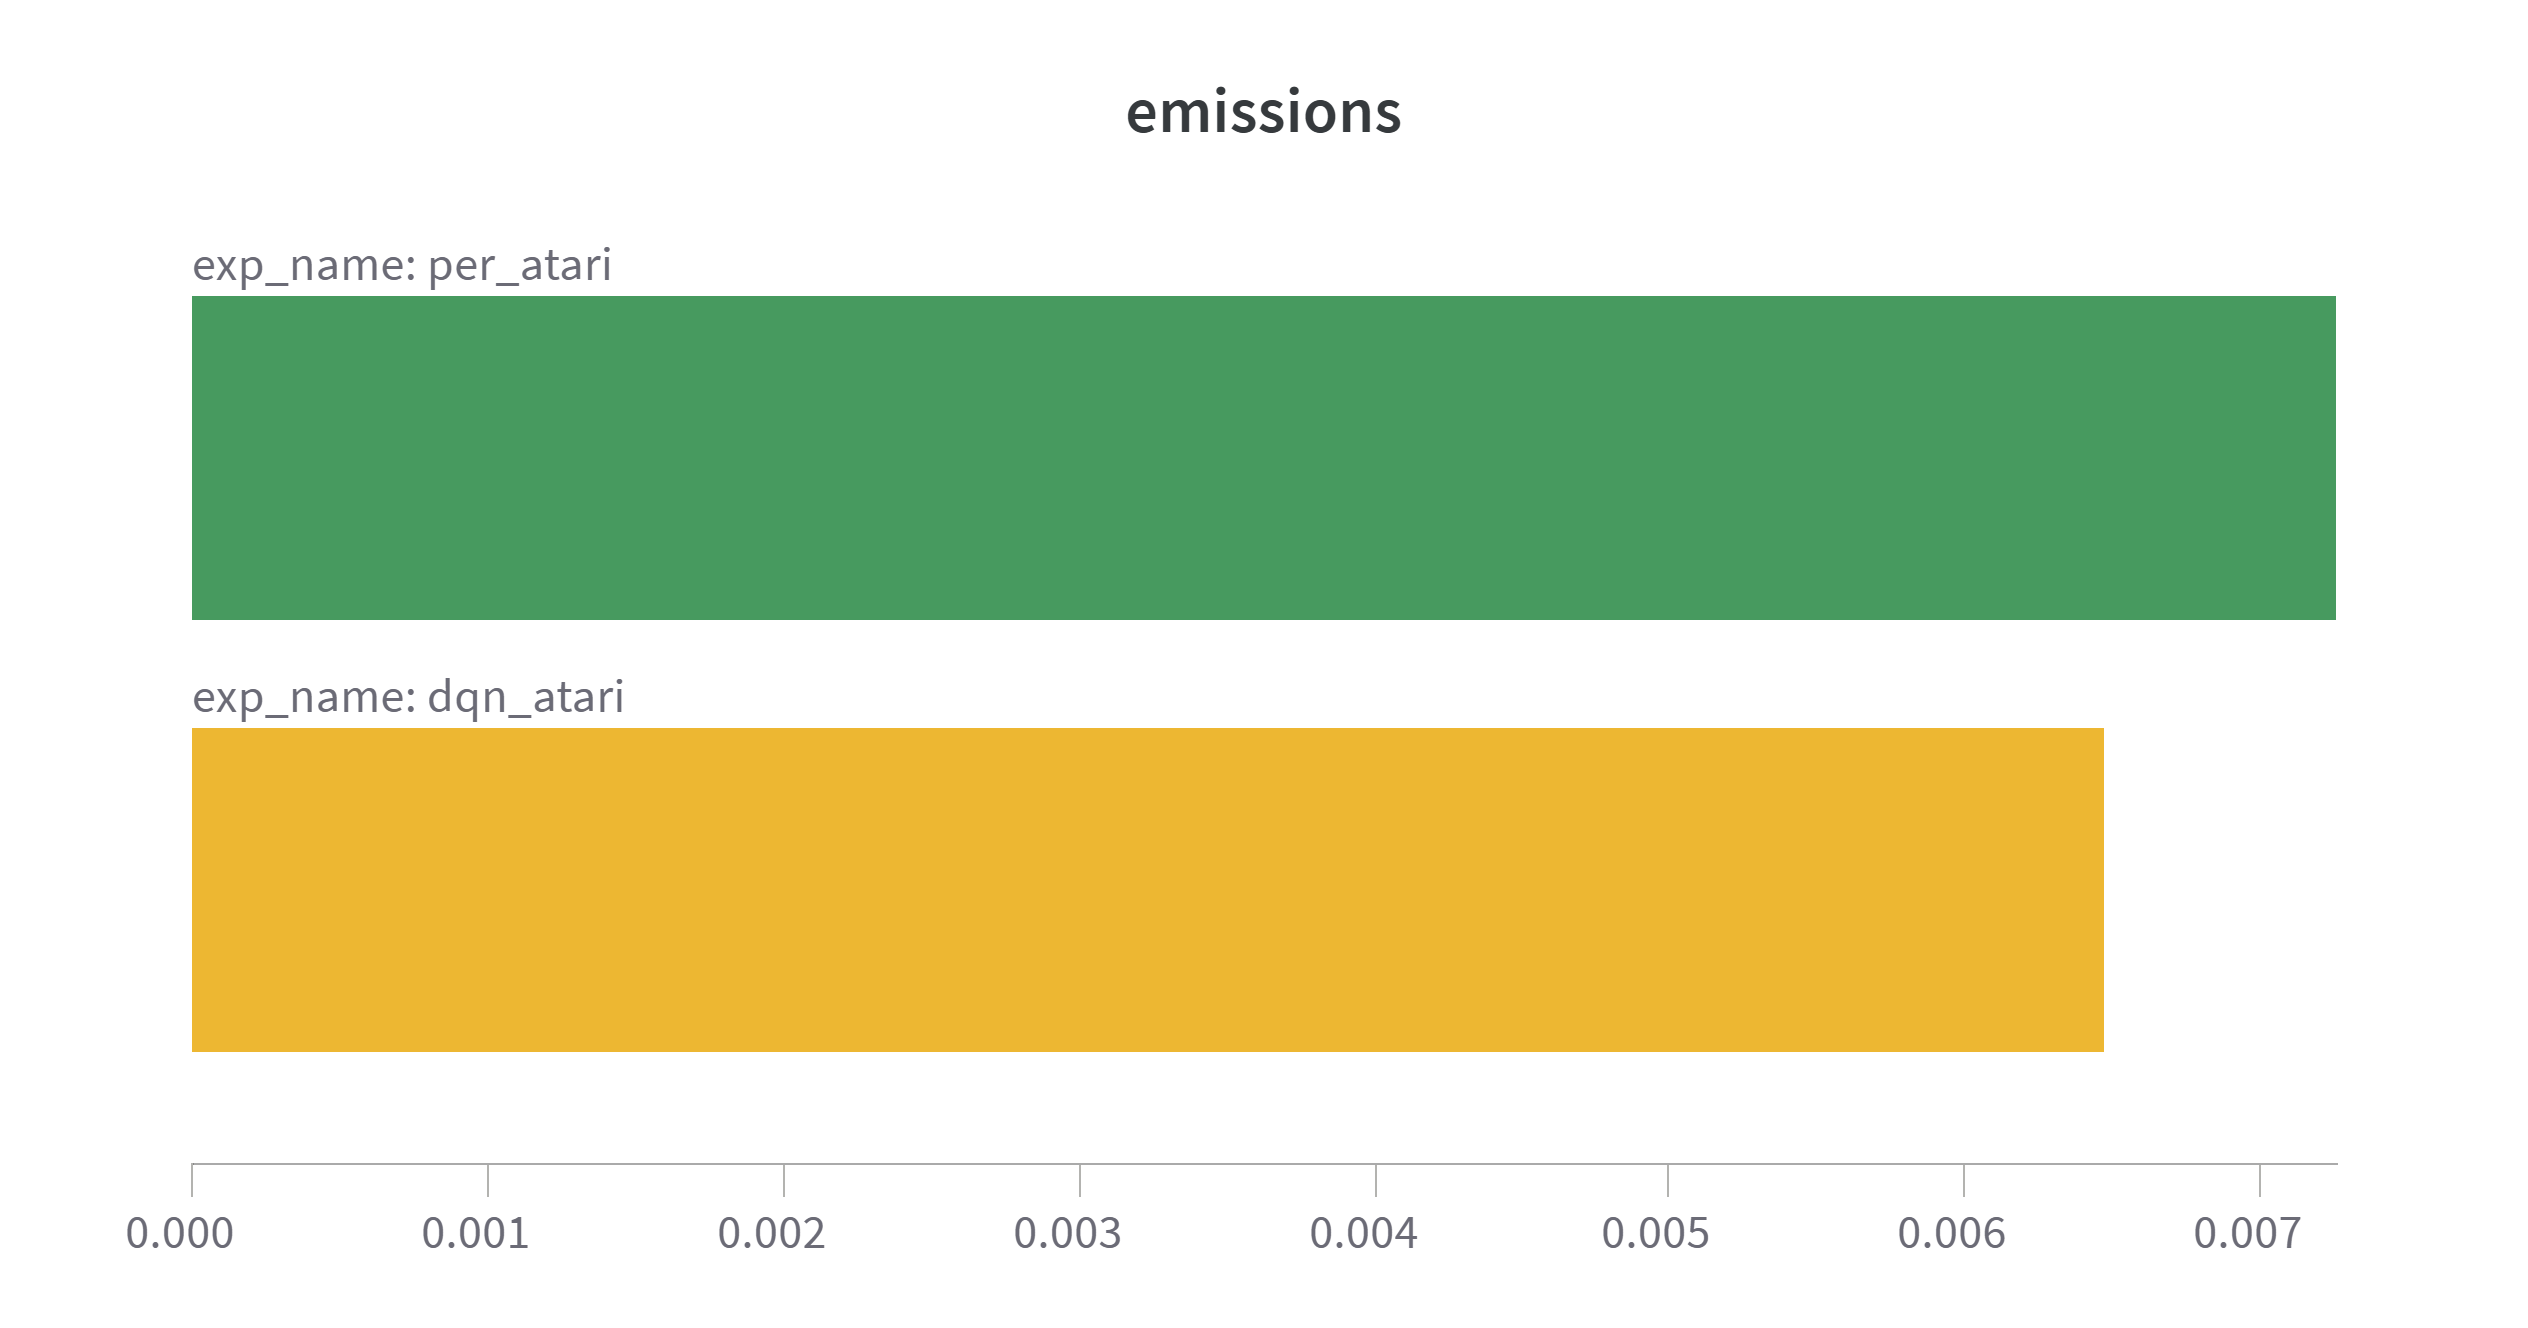
\includegraphics[width=0.55\textwidth]{figures/per/emissions_dqn_per.png}
	\caption{Mean emissions comparison: PER (green) at $\sim0.00725$\,kg vs.\ DQN (gold) at $\sim0.00647$\,kg.}
	\label{fig:per_vs_dqn_emissions}
\end{figure}

\begin{table}
	\caption{Overall final evaluation (10 episodes each) for PER across 32 runs.}
	\label{tab:per_eval_overall}
	\centering
	\begin{tabular}{lcccccccc}
		\toprule
		\textbf{Normalization} & \textbf{mean} & \textbf{std} & \textbf{median} & 
		\textbf{q25} & \textbf{q75} & \textbf{min} & \textbf{max} & \textbf{iqmean} \\
		\midrule
		\textbf{Human}   & 0.0607 & 1.0170 & 0.0539 & 0.0175 & 0.2541 & -10.2619 & 6.8809 & 0.0813 \\
		\textbf{Min--Max}& 0.3533 & 0.2695 & 0.2583 & 0.1499 & 0.6265 & 0.0 & 0.9845 & 0.3087 \\
		\bottomrule
	\end{tabular}
\end{table}

\begin{table}
	\caption{Per-game final evaluation for PER (human- vs.\ min--max normalized). Each row aggregates 10 episodes $\times$ 4 seeds per environment.}
	\label{tab:per_eval_gamewise}
	\centering
	\begin{tabular}{llcccc}
		\toprule
		\textbf{Game} & \textbf{Norm} & \textbf{mean} & \textbf{std} & \textbf{min} & \textbf{max}\\
		\midrule
		Alien     & Human    & 0.0246 & 0.0315 & -0.0147 & 0.0996 \\
		& Min--Max & 0.0978 & 0.0523 & 0.0325  & 0.2225 \\
		\cmidrule{1-6}
		Amidar    & Human    & 0.0263 & 0.0220 & -0.0029 & 0.0809 \\
		& Min--Max & 0.2288 & 0.1693 & 0.0046  & 0.6498 \\
		\cmidrule{1-6}
		Assault   & Human    & 0.2135 & 0.0974 & 0.0232  & 0.3860 \\
		& Min--Max & 0.5648 & 0.1480 & 0.2757  & 0.8270 \\
		\cmidrule{1-6}
		Boxing    & Human    & -0.6667 & 2.7351 & -10.2619 & 6.8809 \\
		& Min--Max & 0.7388  & 0.0890 & 0.4264    & 0.9845 \\
		\cmidrule{1-6}
		Breakout  & Human    & 0.3854 & 0.2204 & 0.00997 & 0.9070 \\
		& Min--Max & 0.3500 & 0.1746 & 0.0526  & 0.7632 \\
		\cmidrule{1-6}
		Freeway   & Human    & 0.4071 & 0.3381 & 0.0     & 0.8446 \\
		& Min--Max & 0.4304 & 0.3574 & 0.0     & 0.8929 \\
		\cmidrule{1-6}
		MsPacman  & Human    & 0.0338 & 0.0111 & 0.0119 & 0.0515 \\
		& Min--Max & 0.2008 & 0.0446 & 0.1126 & 0.2723 \\
		\cmidrule{1-6}
		Pong      & Human    & 0.0617 & 0.0682 & -0.01 & 0.2233 \\
		& Min--Max & 0.2150 & 0.2045 & 0.0   & 0.7000 \\
		\bottomrule
	\end{tabular}
\end{table}

\paragraph{Comparison with Baseline DQN.}
By final evaluation, PER’s overall human-norm mean (0.0607) is lower than DQN’s (0.135), and its min--max mean (0.353) lags behind DQN’s 0.380.  
Figure~\ref{fig:per_vs_dqn_emissions} further shows PER’s emissions exceed DQN’s by $\sim0.0008$\,kg CO\textsubscript{2}-eq on average—likely due to the overhead from prioritized sampling and somewhat longer average episodes.

\paragraph{Observations.}
\begin{itemize}
	\item \textbf{Implementation Details:} 
	We used a \texttt{torch}-based PER buffer to avoid severe slowdowns in the \texttt{numpy} version.
	\item \textbf{Learning Rate:} 
	$\tfrac{1}{4}\times10^{-4}$, as suggested in \cite{schaul:prioritized}, underperformed at 100k steps 
	compared to $1\times10^{-4}$ (Figure~\ref{fig:per_lr_comparison}).
	\item \textbf{Performance:} 
	PER did not consistently outperform baseline DQN within 100k steps: 
	human-norm mean is 0.0607 vs.\ DQN’s 0.135. 
	\item \textbf{Emissions:} 
	PER's overhead leads to slightly higher energy usage (0.00725\,kg CO\textsubscript{2}-eq) than DQN’s 0.00647\,kg.
\end{itemize}

In summary, while prioritizing high-error samples can yield benefits in longer training runs, 
our 100k-step Atari benchmark does not showcase a strong advantage. 
Further hyperparameter tuning or more extended runs might better reveal PER’s strengths.


\subsubsection{Dueling DQN}
\label{subsubsec:dueling_dqn}

\paragraph{(Hyper)Parameters}

\begin{table}
	\caption{Key hyperparameters for Dueling DQN. Only \texttt{env\_id} and \texttt{seed} vary across runs.}
	\label{tab:dueling_dqn_hyperparams}
	\centering
	\begin{tabular}{ll}
		\toprule
		\textbf{Parameter} & \textbf{Value} \\
		\midrule
		\texttt{exp\_name}                & dueling\_dqn\_atari \\
		\texttt{seed}                     & 1..4 \\
		\texttt{torch\_deterministic}     & True \\
		\texttt{cuda}                     & True \\
		\texttt{track}                    & True \\
		\texttt{wandb\_project\_name}     & rlsb \\
		\texttt{capture\_video}           & False \\
		\texttt{save\_model}              & True \\
		\texttt{upload\_model}            & False \\
		\texttt{env\_id}                  & e.g.\ AlienNoFrameskip-v4 \\
		\texttt{total\_timesteps}         & 100000 \\
		\texttt{learning\_rate}           & 0.0001 \\
		\texttt{num\_envs}                & 1 \\
		\texttt{buffer\_size}             & 10000 \\
		\texttt{gamma}                    & 0.99 \\
		\texttt{tau}                      & 1.0 \\
		\texttt{target\_network\_frequency} & 1000 \\
		\texttt{batch\_size}             & 32 \\
		\texttt{start\_e}, \texttt{end\_e} & 1.0 $\to$ 0.01 \\
		\texttt{exploration\_fraction}    & 0.1 \\
		\texttt{learning\_starts}         & 1000 \\
		\texttt{train\_frequency}         & 4 \\
		\bottomrule
	\end{tabular}
\end{table}

\paragraph{Innovation: Dueling Architecture}
The \emph{Dueling DQN}~\cite{wang:dueling} architecture modifies the final layers of a Q-network
to separate the estimation of state-value $V(s)$ from advantage $A(s,a)$.
These two “heads” are combined to yield
\[
Q(s,a) = V(s) + A(s,a) \;-\; \frac{1}{|\mathcal{A}|}\sum_{a'} A(s,a'),
\]
which aims to stabilize learning in states where the choice of action is less critical.

\noindent
\textbf{Network Size Note}:
Because the dueling architecture introduces separate streams for $V$ and $A$, the model ends up
with slightly more parameters. We considered reducing the size of the shared layer to keep the
overall parameter count equal to the baseline, but the difference was only about 512 neurons,
so we retained the original layer size for consistency with the other DQN variants.
We also tested whether gradient clipping (as mentioned in some references) would improve
stability, but found no clear benefit here.
Finally, we did not combine dueling with Double DQN or PER, as our goal is to isolate the contribution
of this single tweak in terms of performance and emissions.

\paragraph{Training Dynamics}

\begin{figure}
	\centering
	\subfloat[][Episodic length. 
	The mean hovers around 3500--4000 steps, with min--max from near 0 up to 8000.]{
		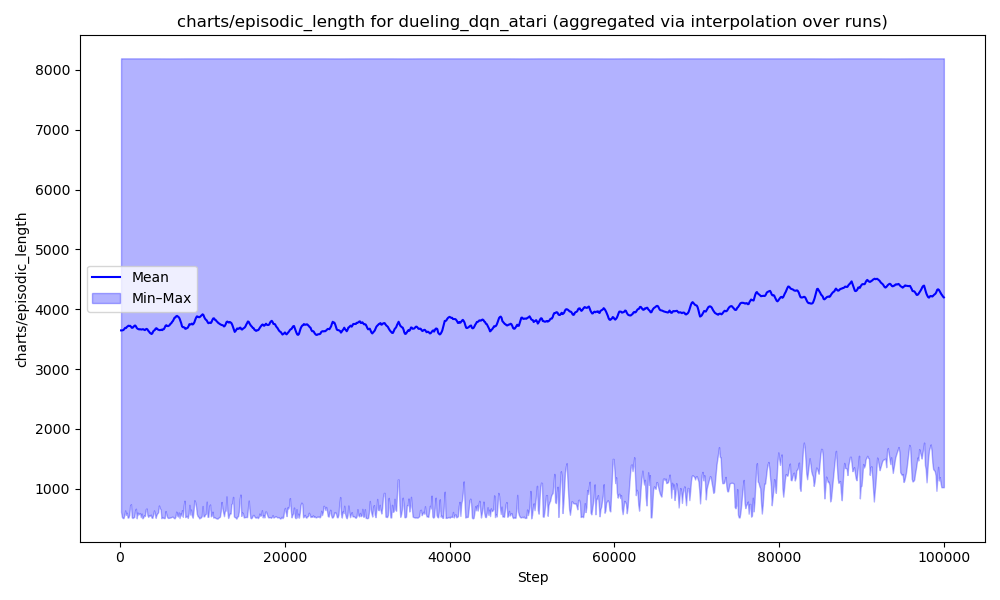
\includegraphics[width=.45\textwidth]{figures/dueling_dqn/charts_episodic_length_dueling_dqn_atari.png}
		\label{fig:dueling_episodic_length}
	}
	\quad
	\subfloat[][Steps per second (SPS). 
	After an initial ramp-up near 170, it stabilizes around 155--160.]{
		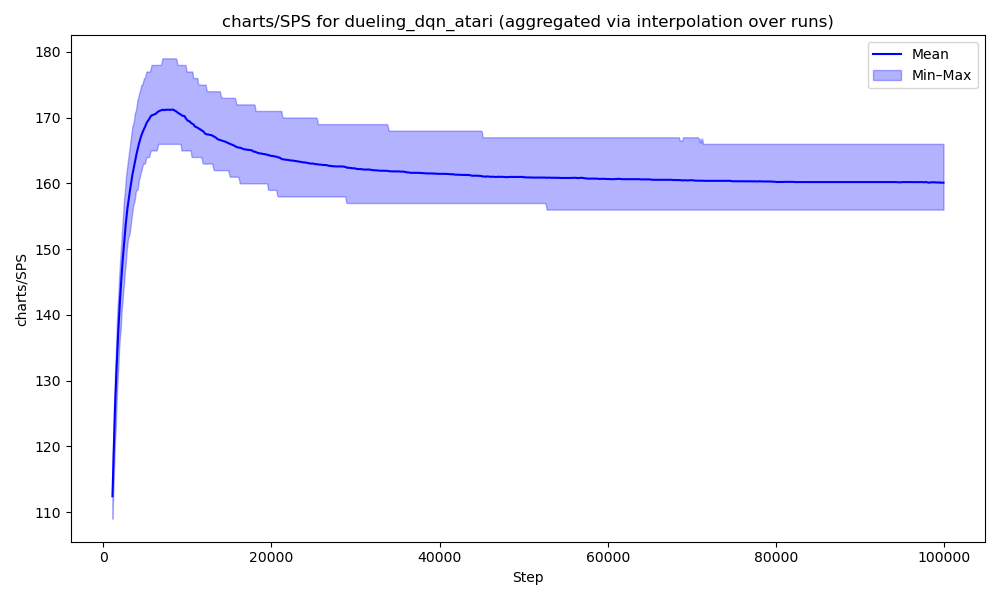
\includegraphics[width=.45\textwidth]{figures/dueling_dqn/charts_SPS_dueling_dqn_atari.png}
		\label{fig:dueling_sps}
	}
	\\[1em]
	\subfloat[][Q-values (\texttt{losses/q\_values}). 
	The mean grows beyond 4--5, with outliers near 8--10.]{
		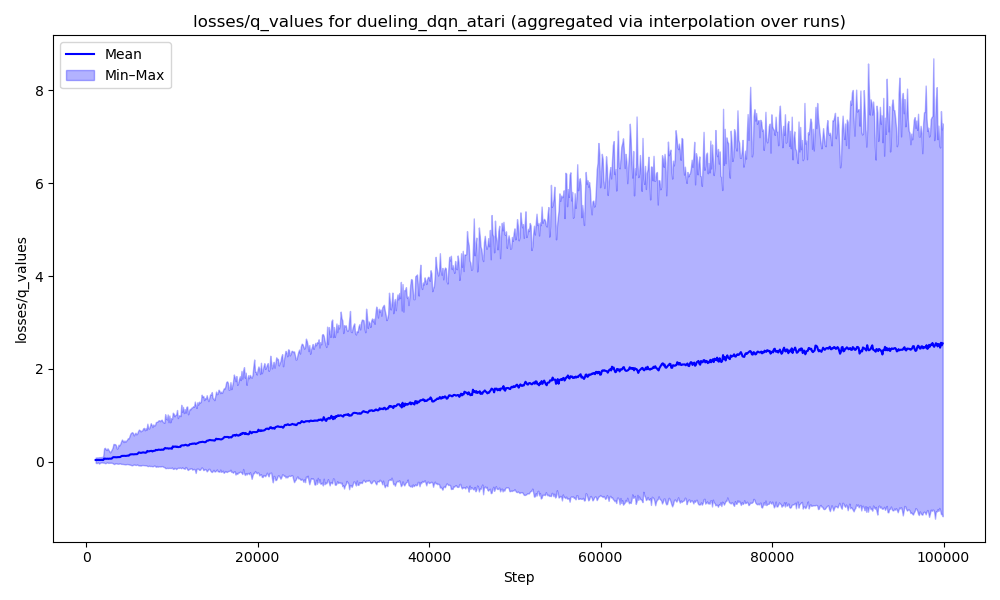
\includegraphics[width=.45\textwidth]{figures/dueling_dqn/losses_q_values_dueling_dqn_atari.png}
		\label{fig:dueling_q_values}
	}
	\quad
	\subfloat[][TD loss (\texttt{losses/td\_loss}). 
	Some runs spike above 1.5--2.0, showing moderate variability late in training.]{
		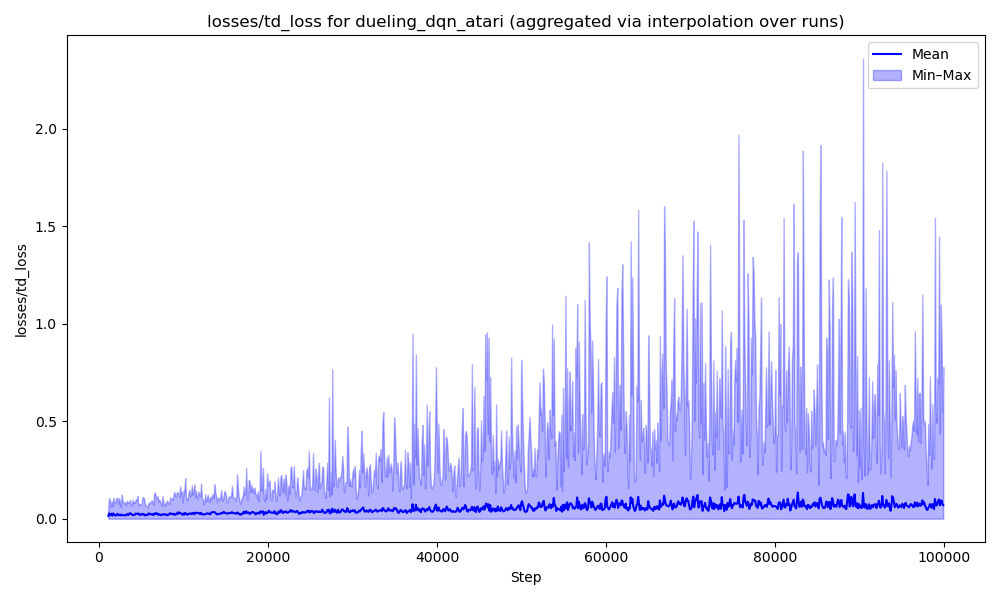
\includegraphics[width=.45\textwidth]{figures/dueling_dqn/losses_td_loss_dueling_dqn_atari.png}
		\label{fig:dueling_td_loss}
	}
	\caption{Dueling DQN training metrics over 100k steps, aggregated over 32 runs.}
	\label{fig:dueling_training_metrics}
\end{figure}

\paragraph{Episodic Return (Aggregated)}

\begin{figure}
	\centering
	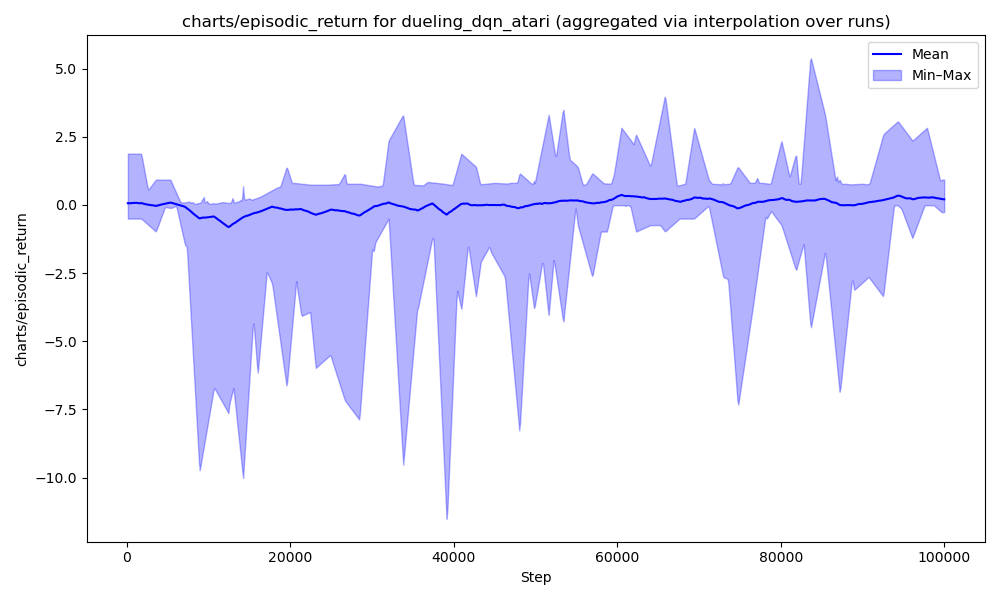
\includegraphics[width=0.6\textwidth]{figures/dueling_dqn/charts_episodic_return_human_dueling_dqn_atari.png}
	\caption{Dueling DQN episodic return (human-normalized) over 100k steps. 
		Variance is significant, with some dips below -8.}
	\label{fig:dueling_return_human}
\end{figure}

\begin{figure}
	\centering
	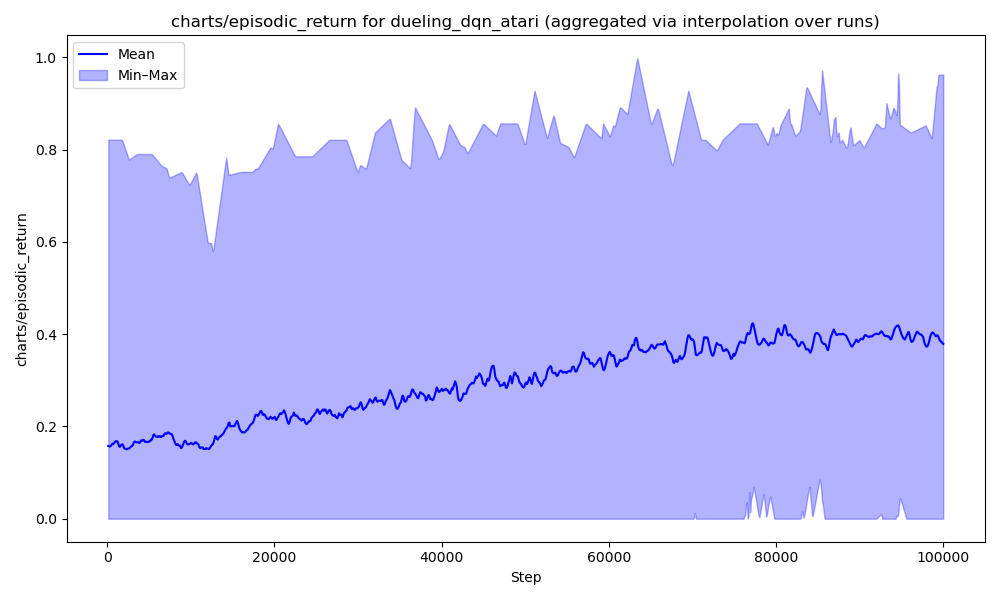
\includegraphics[width=0.6\textwidth]{figures/dueling_dqn/charts_episodic_return_minmax_dueling_dqn_atari.png}
	\caption{Dueling DQN episodic return (min--max normalized) aggregated over 32 runs.}
	\label{fig:dueling_return_minmax}
\end{figure}

\paragraph{Per-Game Returns}

\begin{figure}
	\centering
	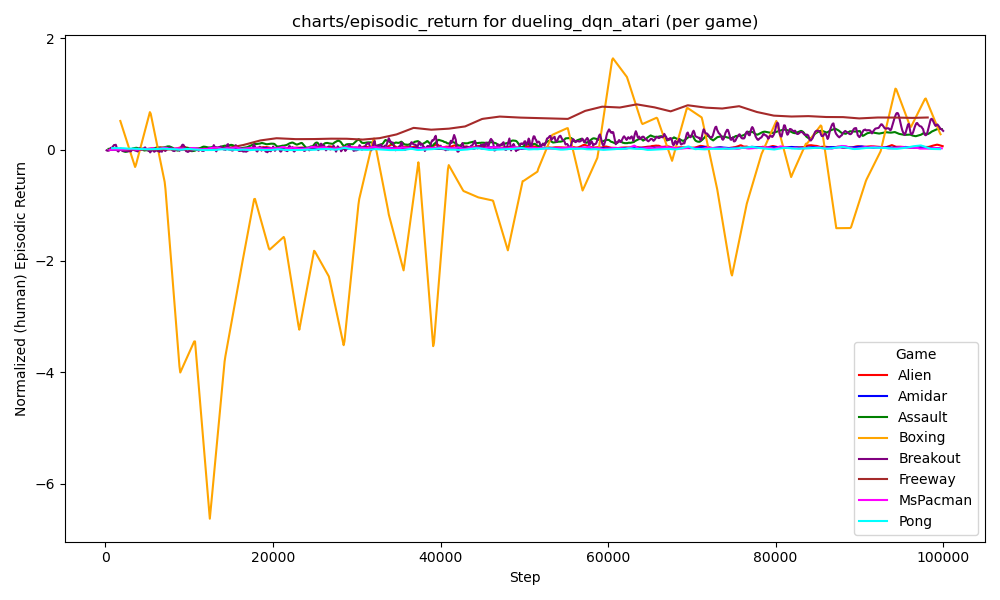
\includegraphics[width=0.6\textwidth]{figures/dueling_dqn/charts_episodic_return_per_game_human_dueling_dqn_atari.png}
	\caption{Dueling DQN returns per game (human-normalized). 
		\emph{Boxing} (orange) experiences deep negative dips, while \emph{Freeway} and \emph{Assault} can reach higher normalized scores.}
	\label{fig:dueling_return_pergame_human}
\end{figure}

\begin{figure}
	\centering
	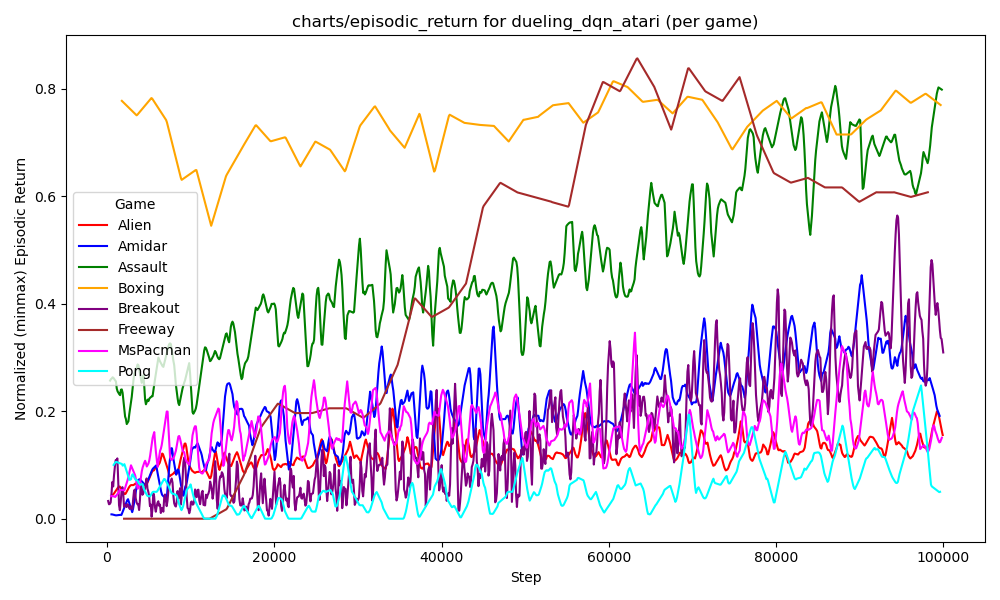
\includegraphics[width=0.6\textwidth]{figures/dueling_dqn/charts_episodic_return_per_game_minmax_dueling_dqn_atari.png}
	\caption{Dueling DQN returns per game (min--max normalized). 
		\emph{Freeway} (gold) and \emph{Assault} (green) often exceed 0.7.}
	\label{fig:dueling_return_pergame_minmax}
\end{figure}

\paragraph{Emissions}

\begin{table}
	\caption{Carbon emissions (kg\,CO\textsubscript{2}eq) for Dueling DQN across 32 runs.}
	\label{tab:dueling_dqn_emissions}
	\centering
	\begin{tabular}{lcccccccc}
		\toprule
		\textbf{Algorithm} & \textbf{mean} & \textbf{std} & \textbf{median} & 
		\textbf{q25} & \textbf{q75} & \textbf{min} & \textbf{max} & \textbf{iqmean} \\
		\midrule
		Dueling DQN & 0.006893 & 0.0002901 & 0.006742 & 0.006672 & 0.007002 & 0.006617 & 0.007478 & 0.006779 \\
		\bottomrule
	\end{tabular}
\end{table}

\begin{figure}
	\centering
	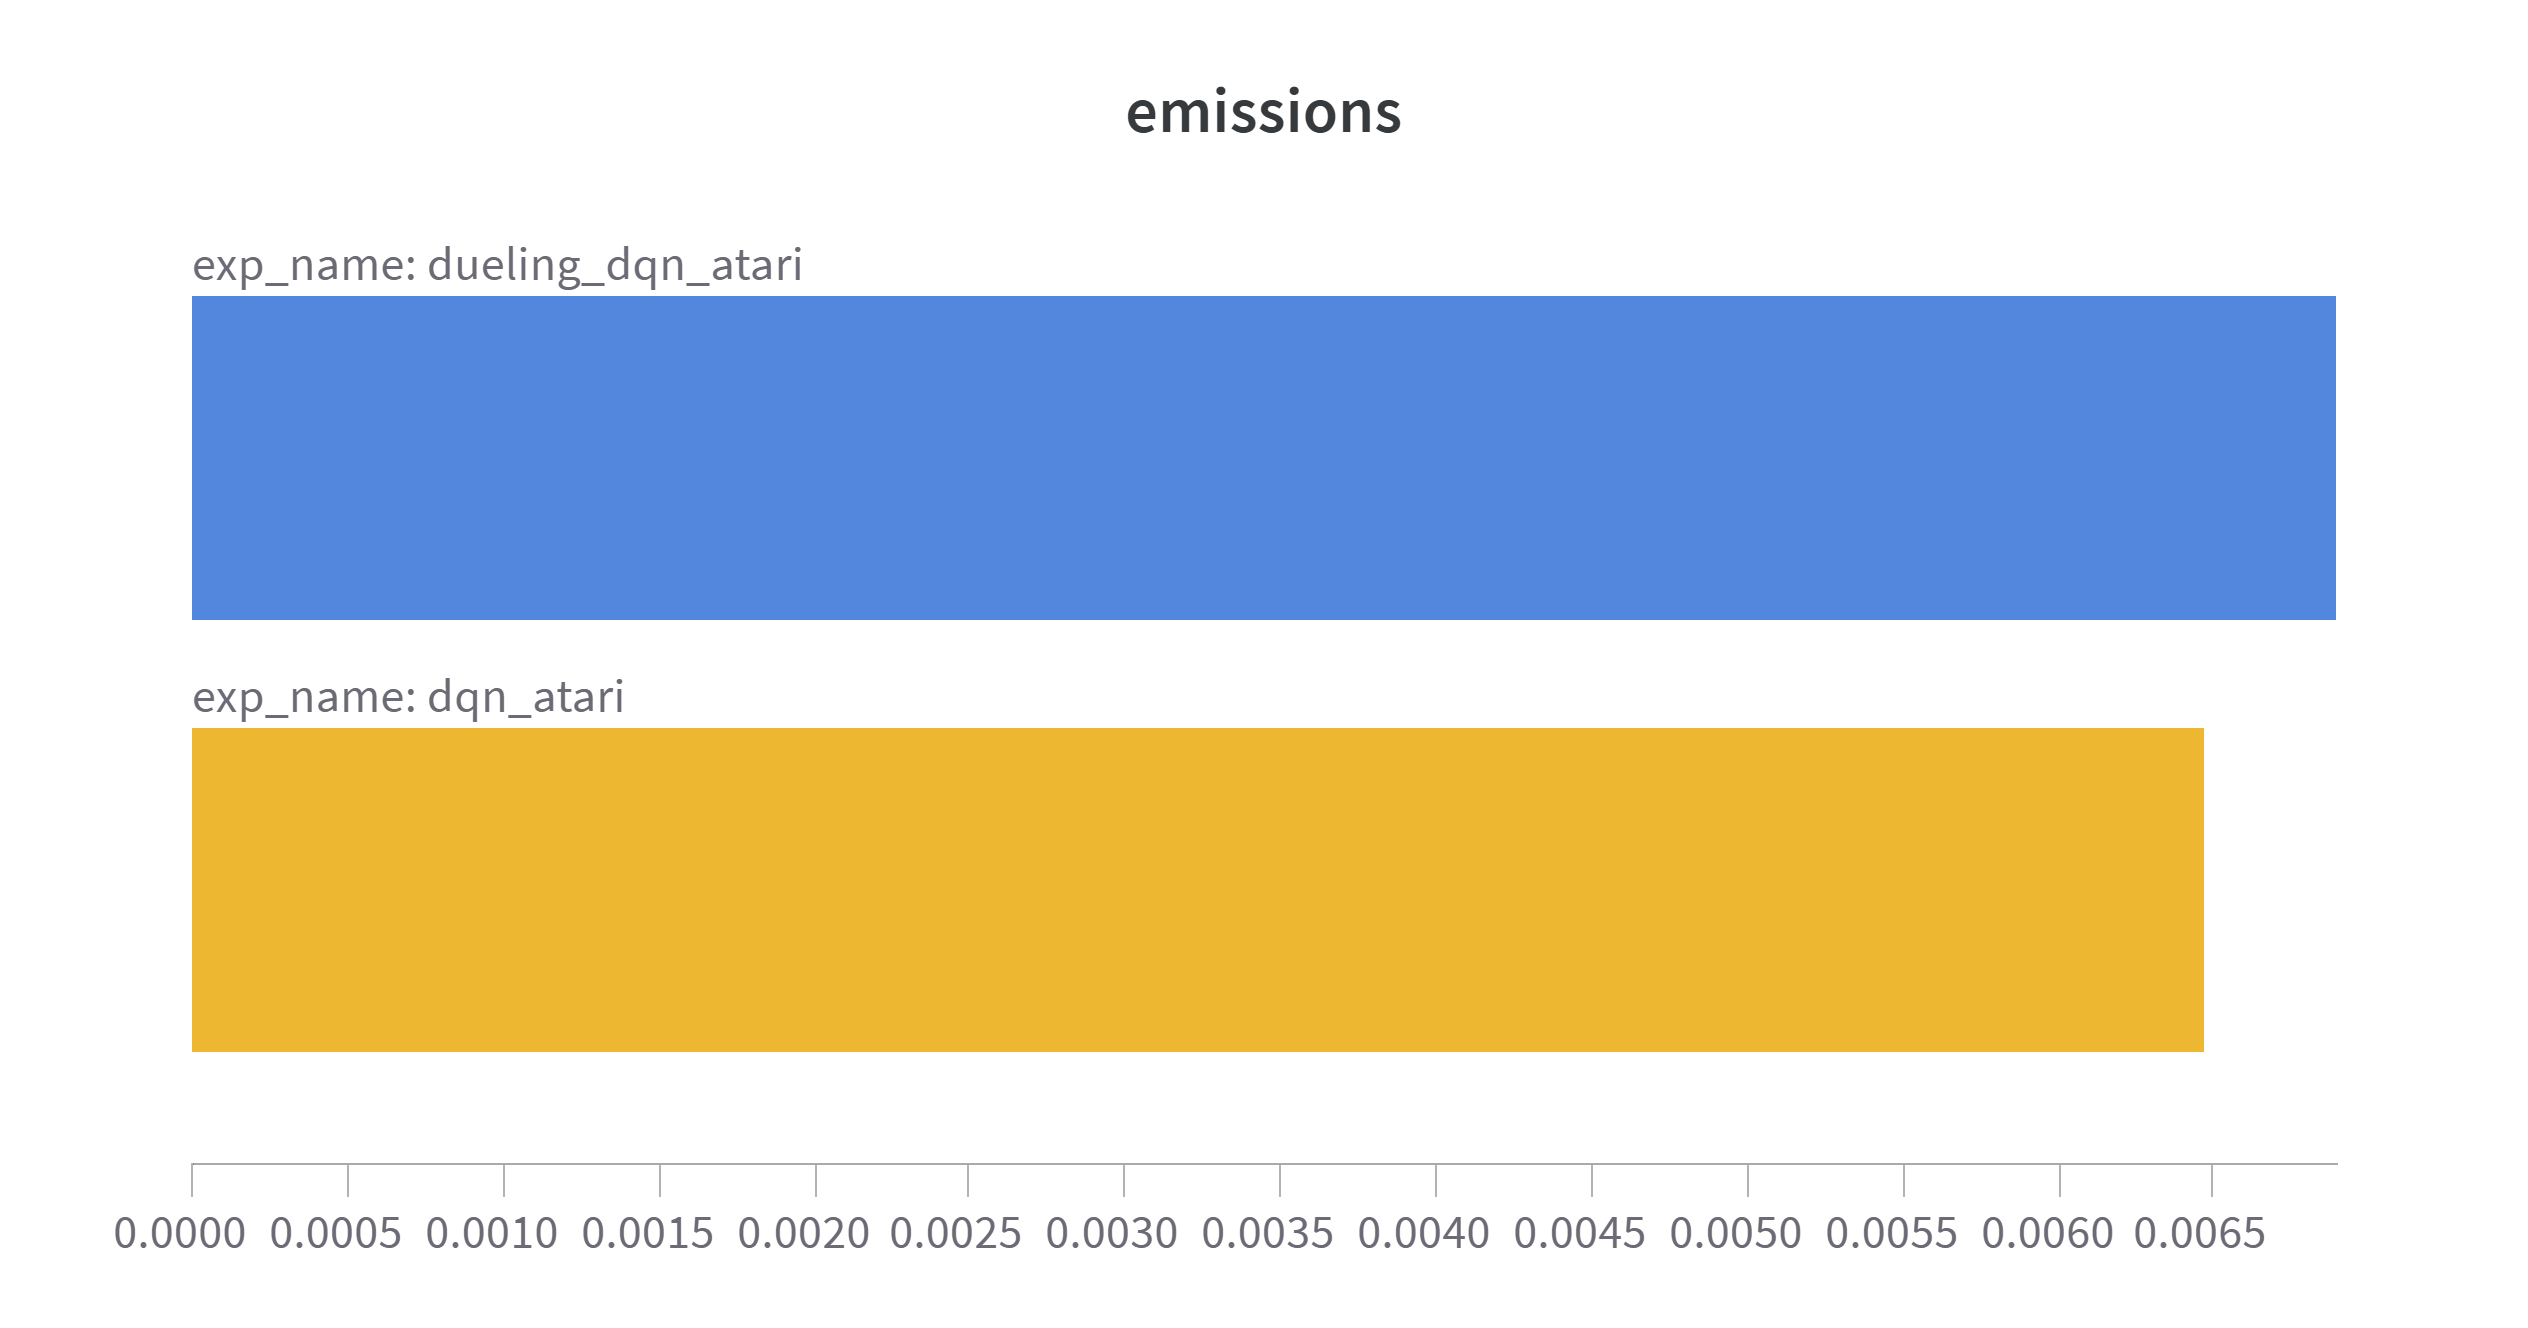
\includegraphics[width=0.55\textwidth]{figures/dueling_dqn/emissions_dqn_dueling.png}
	\caption{Mean emissions comparison: Dueling DQN (blue) at $\sim0.00689$\,kg vs.\ DQN (gold) at $\sim0.00647$\,kg.}
	\label{fig:dueling_emissions_barplot}
\end{figure}

\paragraph{Evaluation Results}

\begin{table}
	\caption{Overall final evaluation (10 episodes each) for Dueling DQN across 32 runs.}
	\label{tab:dueling_dqn_eval_overall}
	\centering
	\begin{tabular}{lcccccccc}
		\toprule
		\textbf{Normalization} & \textbf{mean} & \textbf{std} & \textbf{median} & 
		\textbf{q25} & \textbf{q75} & \textbf{min} & \textbf{max} & \textbf{iqmean} \\
		\midrule
		\textbf{Human}   & 0.1860 & 0.5258 & 0.0402 & 0.0148 & 0.3530 & -1.9286 & 3.5476 & 0.1020 \\
		\textbf{Min--Max}& 0.3849 & 0.3056 & 0.2632 & 0.1100 & 0.7448 & 0.0 & 0.9523 & 0.3454 \\
		\bottomrule
	\end{tabular}
\end{table}

\begin{table}
	\caption{Per-game final evaluation for Dueling DQN (human- vs.\ min--max normalized).}
	\label{tab:dueling_dqn_eval_gamewise}
	\centering
	\begin{tabular}{llcccc}
		\toprule
		\textbf{Game} & \textbf{Norm} & \textbf{mean} & \textbf{std} & \textbf{min} & \textbf{max}\\
		\midrule
		Alien     & Human    & 0.0398 & 0.0346 & -0.0072 & 0.1493 \\
		& Min--Max & 0.1231 & 0.0574 & 0.0450  & 0.3050 \\
		\cmidrule{1-6}
		Amidar    & Human    & 0.0372 & 0.0193 & 0.0235 & 0.0935 \\
		& Min--Max & 0.3127 & 0.1482 & 0.2074 & 0.7465 \\
		\cmidrule{1-6}
		Assault   & Human    & 0.3200 & 0.0985 & 0.1057 & 0.4684 \\
		& Min--Max & 0.7266 & 0.1498 & 0.4010 & 0.9523 \\
		\cmidrule{1-6}
		Boxing    & Human    & 0.1190 & 1.3282 & -1.9286 & 3.5476 \\
		& Min--Max & 0.7643 & 0.0432 & 0.6977  & 0.8760 \\
		\cmidrule{1-6}
		Breakout  & Human    & 0.4020 & 0.2904 & -0.0565 & 1.0066 \\
		& Min--Max & 0.3632 & 0.2300 & 0.0     & 0.8421 \\
		\cmidrule{1-6}
		Freeway   & Human    & 0.5372 & 0.3162 & 0.0     & 0.7770 \\
		& Min--Max & 0.5679 & 0.3342 & 0.0     & 0.8214 \\
		\cmidrule{1-6}
		MsPacman  & Human    & 0.0265 & 0.0204 & 0.00018 & 0.0736 \\
		& Min--Max & 0.1713 & 0.0823 & 0.0654  & 0.3613 \\
		\cmidrule{1-6}
		Pong      & Human    & 0.0067 & 0.0185 & -0.01 & 0.0567 \\
		& Min--Max & 0.0500 & 0.0555 & 0.0   & 0.2 \\
		\bottomrule
	\end{tabular}
\end{table}

\paragraph{Comparison with Baseline DQN}
In final evaluation, Dueling DQN’s \emph{human}-norm mean is 0.1860 vs.\ DQN’s 0.1353, 
and the \emph{min--max} mean is 0.3849 vs.\ DQN’s 0.3802—so we see a small positive difference on average.
However, \emph{Boxing} outliers (some runs exceed 3.5, others dip below $-1.9$) inflate the variance.
Meanwhile, emissions at $\sim0.00689$\,kg CO\textsubscript{2}-eq are higher than DQN’s $\sim0.00647$ but remain
lower than some other variants (e.g.\ PER at 0.00725).

\paragraph{Observations}
\begin{itemize}
	\item \textbf{Architecture Impact:}
	The \emph{dueling} approach separates state-value and advantage,
	intending to stabilize updates in states where action choices matter less.
	\item \textbf{Network Size:}
	We kept the same shared layer size as DQN, adding only a modest number of extra parameters.
	\item \textbf{Performance:}
	The final mean in human normalization (0.1860) is higher than baseline DQN’s 0.1353,
	though min--max (0.3849 vs.\ 0.3802) is only slightly larger.
	\item \textbf{Emissions:}
	Dueling DQN uses $\sim0.00689$\,kg CO\textsubscript{2}-eq,
	more than DQN’s 0.00647 but less than PER’s 0.00725.
\end{itemize}


\subsubsection{Categorical DQN (C51)}
\label{subsubsec:c51}

\paragraph{(Hyper)Parameters}

\begin{table}
	\caption{Key hyperparameters for the C51 algorithm. Only \texttt{env\_id} and \texttt{seed} vary across runs.}
	\label{tab:c51_hyperparams}
	\centering
	\begin{tabular}{ll}
		\toprule
		\textbf{Parameter} & \textbf{Value} \\
		\midrule
		\texttt{exp\_name}                & c51\_atari \\
		\texttt{seed}                     & 1..4 \\
		\texttt{torch\_deterministic}     & True \\
		\texttt{cuda}                     & True \\
		\texttt{track}                    & True \\
		\texttt{wandb\_project\_name}     & rlsb \\
		\texttt{capture\_video}           & False \\
		\texttt{save\_model}              & True \\
		\texttt{upload\_model}            & False \\
		\texttt{env\_id}                  & e.g.\ AlienNoFrameskip-v4 \\
		\texttt{total\_timesteps}         & 100000 \\
		\texttt{learning\_rate}           & 0.00025 \\
		\texttt{num\_envs}                & 1 \\
		\texttt{n\_atoms}                 & 51 \\
		\texttt{v\_min}                   & -10 \\
		\texttt{v\_max}                   & 10 \\
		\texttt{buffer\_size}             & 10000 \\
		\texttt{gamma}                    & 0.99 \\
		\texttt{target\_network\_frequency} & 1000 \\
		\texttt{batch\_size}             & 32 \\
		\texttt{start\_e}, \texttt{end\_e} & 1.0 $\to$ 0.01 \\
		\texttt{exploration\_fraction}    & 0.1 \\
		\texttt{learning\_starts}         & 1000 \\
		\texttt{train\_frequency}         & 4 \\
		\bottomrule
	\end{tabular}
\end{table}

\paragraph{Innovation: Distributional RL}
Categorical DQN (\textbf{C51})~\cite{bellemare:distributional} models $Q(s,a)$ 
as a discrete probability distribution over possible returns, using $\texttt{n\_atoms}$ support points 
that span the interval $[v_{\mathrm{min}},\,v_{\mathrm{max}}]$. 
By capturing more than a single expected value, C51 can potentially improve learning stability 
and performance, especially in risk- or variance-sensitive tasks.

\paragraph{Hyperparameter Tuning}
We adopted CleanRL’s \texttt{c51\_atari} configuration with 51 atoms, $v_{\min}=-10$, $v_{\max}=10$, 
and a learning rate of $2.5\times10^{-4}$. While we tested alternative rates, 
this default proved effective over only 100k steps.  

We also experimented with \texttt{target\_network\_frequency} values of 1k, 5k, and 10k 
to see if less frequent updates might reduce overhead. 
Ultimately, 1k provided a good balance of stable returns and moderate emissions, 
aligning with other DQN-based variants.

\paragraph{Training Dynamics}

\begin{figure}
	\centering
	\subfloat[][Episodic length (\texttt{charts\_episodic\_length}). 
	The mean is \(\sim 3500\)--\(4000\), while min--max occasionally spikes above 8000 or even 17500 in some runs.]{
		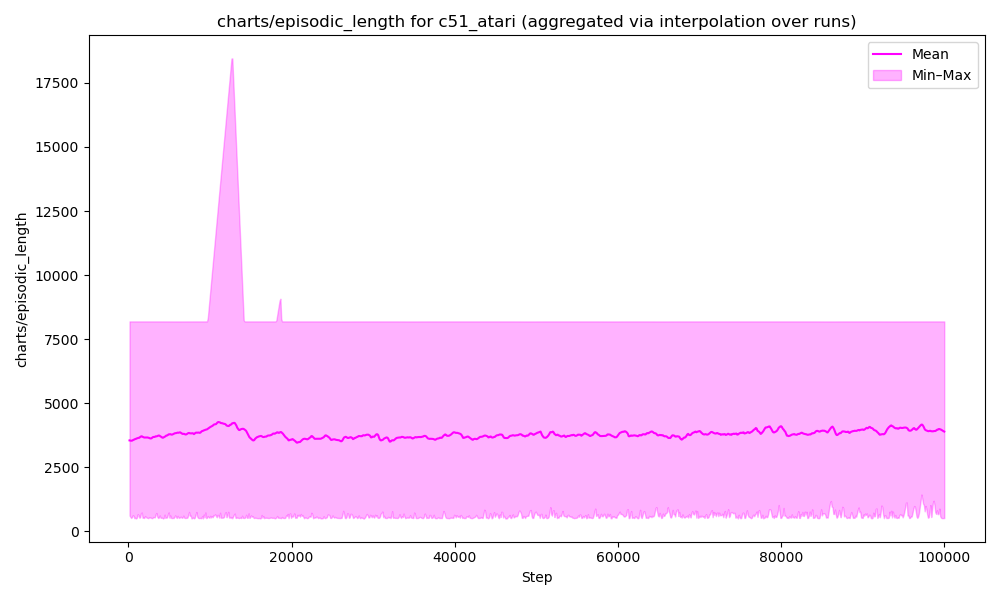
\includegraphics[width=.45\textwidth]{figures/c51/charts_episodic_length_c51_atari.png}
		\label{fig:c51_episodic_length}
	}
	\quad
	\subfloat[][Steps per second (SPS).
	Mean peaks around 160--170, then slowly converges near 140--150.]{
		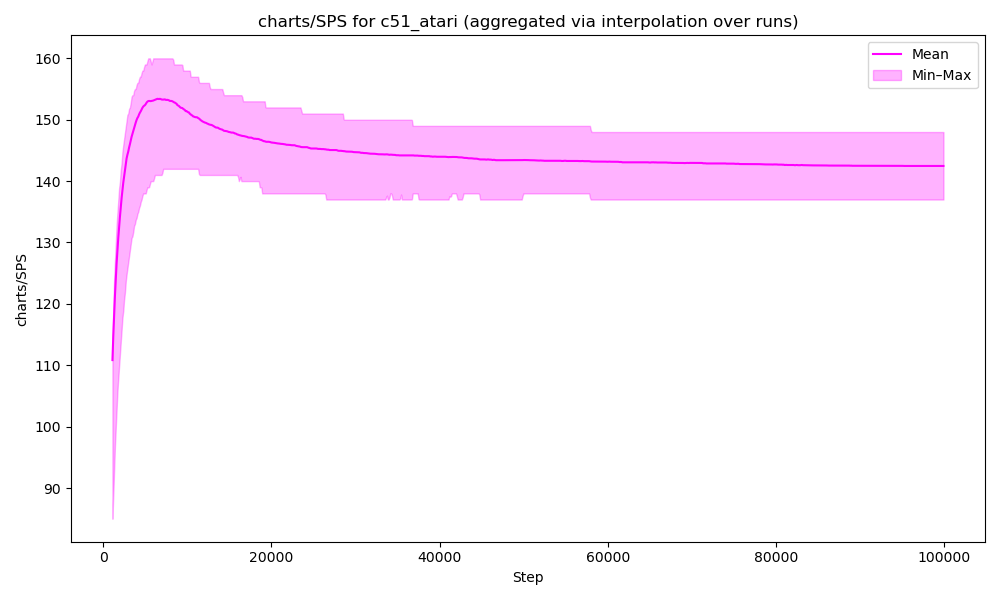
\includegraphics[width=.45\textwidth]{figures/c51/charts_SPS_c51_atari.png}
		\label{fig:c51_sps}
	}
	\\[1em]
	\subfloat[][Overall loss (\texttt{losses/loss}). 
	The mean steadily declines from about 4.0 toward near 2.0 by the end of training.]{
		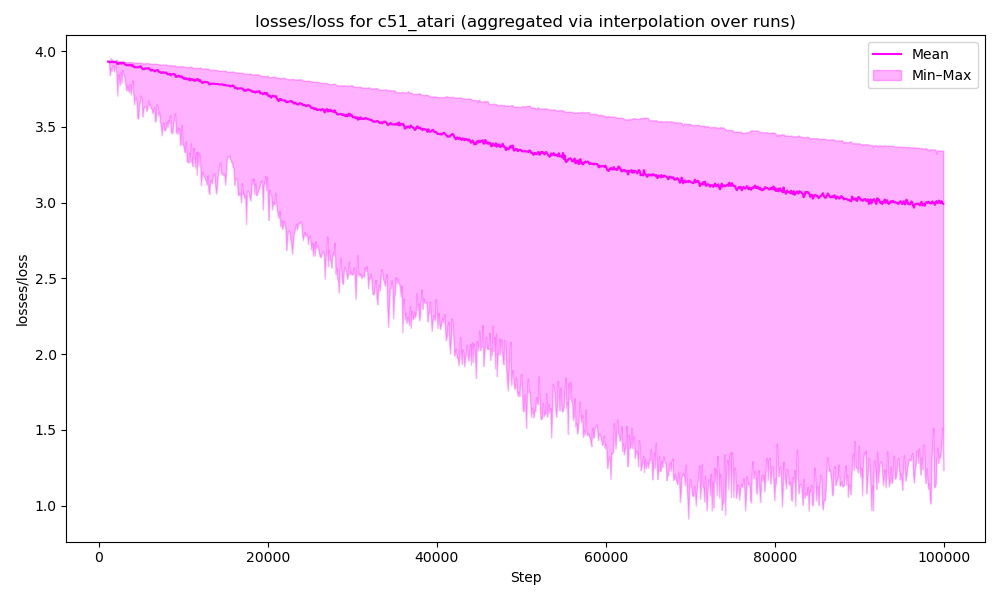
\includegraphics[width=.45\textwidth]{figures/c51/losses_loss_c51_atari.png}
		\label{fig:c51_loss}
	}
	\quad
	\subfloat[][Q-values (\texttt{losses/q\_values}). 
	The mean climbs from near 0 to $\sim 4$--$5$, with outliers reaching 6--7.]{
		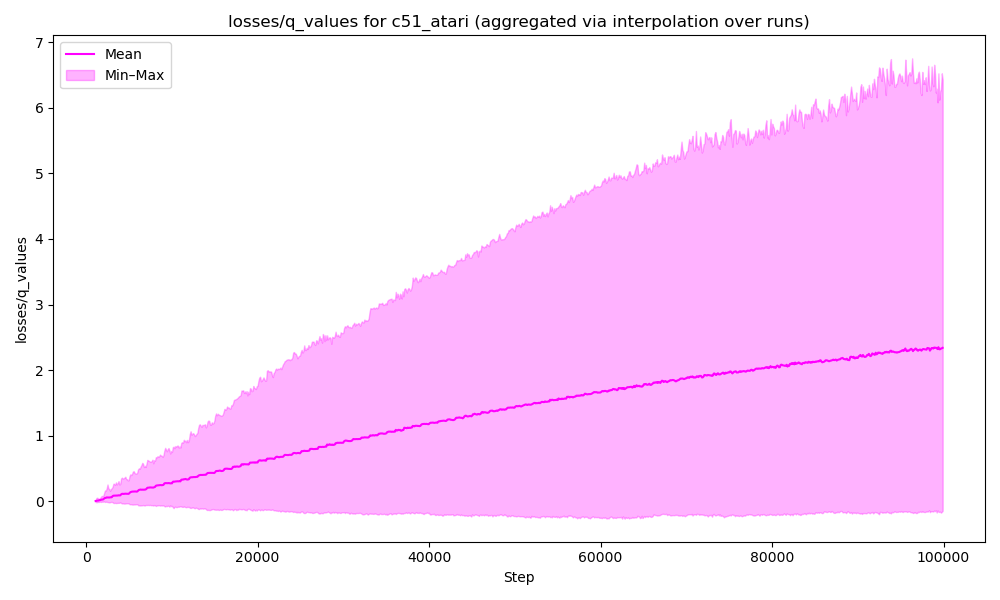
\includegraphics[width=.45\textwidth]{figures/c51/losses_q_values_c51_atari.png}
		\label{fig:c51_q_values}
	}
	\caption{C51 training metrics over 100k steps, aggregated (via interpolation) across 32 runs.}
	\label{fig:c51_training_metrics}
\end{figure}

Figure~\ref{fig:c51_training_metrics} shows that certain runs produce extremely long episodes 
(Figure~\ref{fig:c51_episodic_length}, subfloat~a), 
while the overall \texttt{SPS} curve (subfloat~b) hovers around 140--150 later in training, 
slightly lower than baseline DQN’s $\sim160$. 
The training loss (subfloat~c) descends from near 4.0 to 2.0, 
while distributional \texttt{q\_values} (subfloat~d) broaden significantly.

\paragraph{Episodic Return (Aggregated)}

\begin{figure}
	\centering
	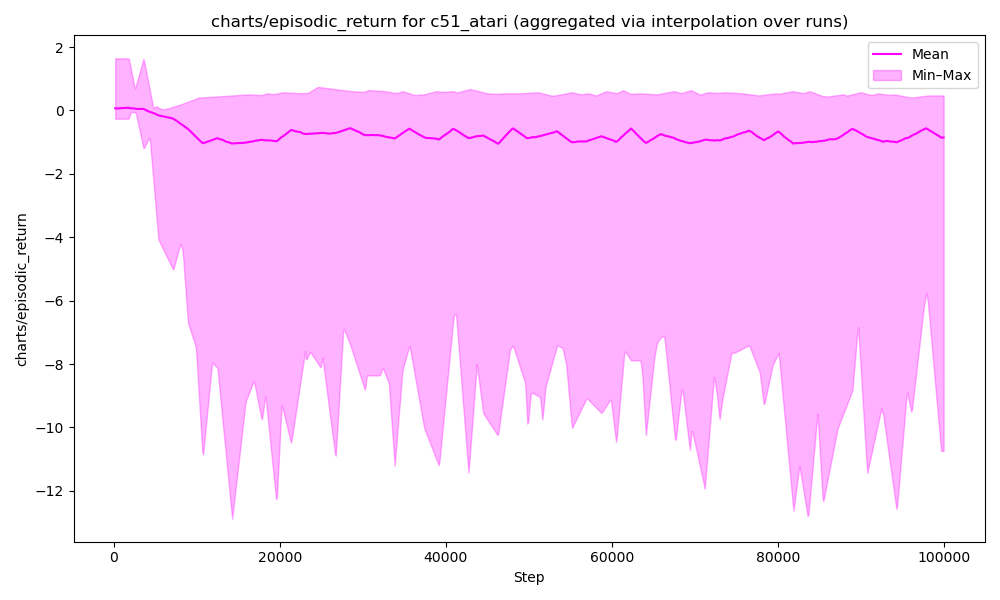
\includegraphics[width=0.6\textwidth]{figures/c51/charts_episodic_return_human_c51_atari.png}
	\caption{C51 episodic return (human-normalized), aggregated over 32 runs. 
		Negative scores dominate, especially due to \emph{Boxing}’s steep dips below -10.}
	\label{fig:c51_return_human}
\end{figure}

\begin{figure}
	\centering
	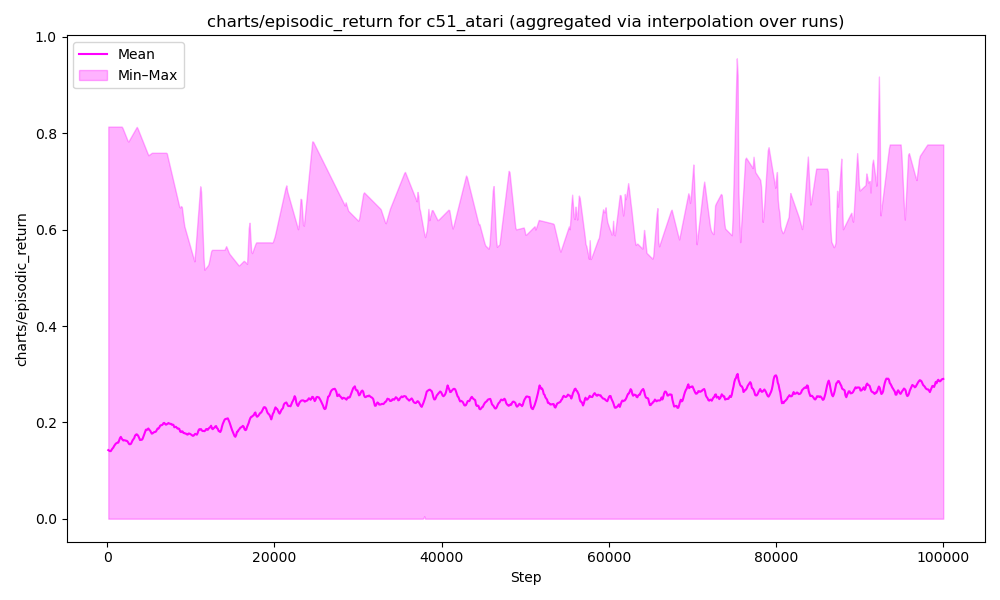
\includegraphics[width=0.6\textwidth]{figures/c51/charts_episodic_return_minmax_c51_atari.png}
	\caption{C51 episodic return (min--max normalized). 
		The mean grows toward 0.25--0.30, indicating moderate performance relative to each game’s min--max range.}
	\label{fig:c51_return_minmax}
\end{figure}

Due to extreme negative performance in certain games, such as \emph{Boxing}, 
the human-normalized return (Figure~\ref{fig:c51_return_human}) 
often falls below -1. In min--max (Figure~\ref{fig:c51_return_minmax}), 
the mean approaches $\sim0.25$--$0.30$ by 100k steps.

\paragraph{Per-Game Returns}

\begin{figure}
	\centering
	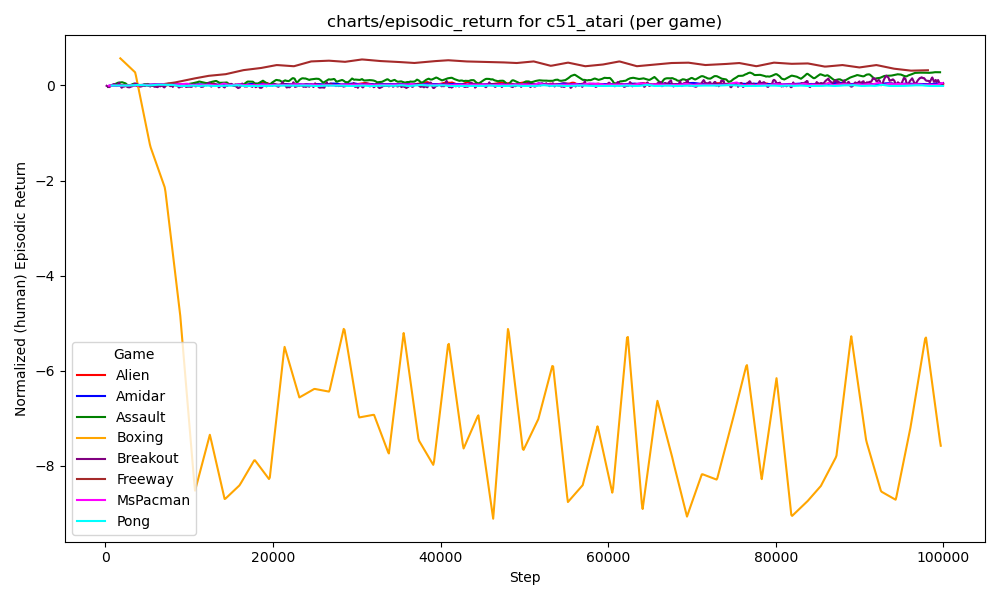
\includegraphics[width=0.6\textwidth]{figures/c51/charts_episodic_return_per_game_human_c51_atari.png}
	\caption{C51 returns per game (human-normalized). 
		\emph{Boxing} (orange) can plunge below -12, dwarfing improvements in other games.}
	\label{fig:c51_return_pergame_human}
\end{figure}

\begin{figure}
	\centering
	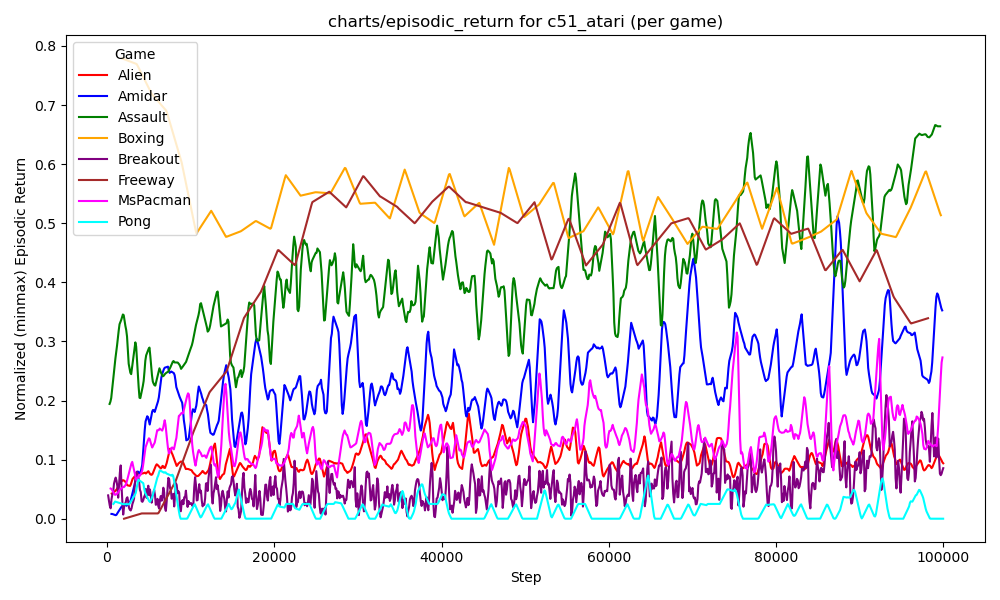
\includegraphics[width=0.6\textwidth]{figures/c51/charts_episodic_return_per_game_minmax_c51_atari.png}
	\caption{C51 returns per game (min--max normalized). 
		\emph{Assault} (green) climbs above 0.5, while \emph{Pong} (cyan) remains near zero.}
	\label{fig:c51_return_pergame_minmax}
\end{figure}

\paragraph{Emissions}

\begin{table}
	\caption{Carbon emissions (kg\,CO\textsubscript{2}eq) for C51 across 32 runs.}
	\label{tab:c51_emissions}
	\centering
	\begin{tabular}{lcccccccc}
		\toprule
		\textbf{Algorithm} & \textbf{mean} & \textbf{std} & \textbf{median} & 
		\textbf{q25} & \textbf{q75} & \textbf{min} & \textbf{max} & \textbf{iqmean} \\
		\midrule
		C51 & 0.007750 & 0.0003042 & 0.007655 & 0.007489 & 0.008099 & 0.007410 & 0.008257 & 0.007679 \\
		\bottomrule
	\end{tabular}
\end{table}

\begin{figure}
	\centering
	\includegraphics[width=0.55\textwidth]{figures/c51/emissions_dqn_c51.png}
	\caption{Mean emissions: C51 (magenta) at $\sim0.00775$\,kg vs.\ DQN (gold) at $\sim0.00647$\,kg.}
	\label{fig:c51_vs_dqn_emissions}
\end{figure}

C51’s mean emissions near 0.00775\,kg exceed DQN’s 0.00647\,kg. 
Distributional overhead (computing 51 probability “atoms”) likely increases GPU usage.

\paragraph{Evaluation Results}

\begin{table}
	\caption{Overall final evaluation (10 episodes each) for C51 across 32 runs.}
	\label{tab:c51_eval_overall}
	\centering
	\begin{tabular}{lcccccccc}
		\toprule
		\textbf{Normalization} & \textbf{mean} & \textbf{std} & \textbf{median} & 
		\textbf{q25} & \textbf{q75} & \textbf{min} & \textbf{max} & \textbf{iqmean} \\
		\midrule
		\textbf{Human}   & -1.0811 & 3.2862 & 0.0 & -0.0132 & 0.0418 & -12.8810 & 0.7770 & 0.00684 \\
		\textbf{Min--Max}& 0.2503 & 0.2568 & 0.2005 & 0.0 & 0.4419 & 0.0 & 0.8270 & 0.13997 \\
		\bottomrule
	\end{tabular}
\end{table}

\begin{table}
	\caption{Per-game final evaluation for C51 (human- vs.\ min--max normalized). 
		Each row aggregates 40 total episodes (10 per seed).}
	\label{tab:c51_eval_gamewise}
	\centering
	\begin{tabular}{llcccc}
		\toprule
		\textbf{Game} & \textbf{Norm} & \textbf{mean} & \textbf{std} & \textbf{min} & \textbf{max}\\
		\midrule
		Alien & Human    & -0.0149 & 0.0127 & -0.0343 & 0.00635 \\
		& Min--Max & 0.0321  & 0.0211 & 0.0     & 0.0675 \\
		\cmidrule{1-6}
		Amidar & Human   & 0.0336  & 0.0153 & 0.00431 & 0.0678 \\
		& Min--Max & 0.2851 & 0.1181 & 0.0599  & 0.5484 \\
		\cmidrule{1-6}
		Assault & Human  & 0.1994  & 0.1467 & -0.0262 & 0.3860 \\
		& Min--Max & 0.5434 & 0.2229 & 0.2005  & 0.8270 \\
		\cmidrule{1-6}
		Boxing & Human   & -9.3869 & 2.6728 & -12.8810 & -4.7857 \\
		& Min--Max & 0.4548  & 0.0870 & 0.3411   & 0.6047 \\
		\cmidrule{1-6}
		Breakout & Human & 0.1478  & 0.2072 & -0.0565 & 0.4751 \\
		& Min--Max & 0.1618 & 0.1641 & 0.0     & 0.4211 \\
		\cmidrule{1-6}
		Freeway & Human  & 0.3632  & 0.3688 & 0.0      & 0.7770 \\
		& Min--Max & 0.3839 & 0.3899 & 0.0     & 0.8214 \\
		\cmidrule{1-6}
		MsPacman & Human & 0.0189  & 0.0176 & -0.0057 & 0.0483 \\
		& Min--Max & 0.1410 & 0.0707 & 0.0419 & 0.2592 \\
		\cmidrule{1-6}
		Pong & Human     & -0.01   & $5.27\times 10^{-18}$ & -0.01 & -0.01 \\
		& Min--Max & 0.0     & 0.0     & 0.0     & 0.0 \\
		\bottomrule
	\end{tabular}
\end{table}

\paragraph{Comparison with Baseline DQN}
Overall, C51’s human-normalized final mean is \textbf{-1.0811}, pulled down by severe negative performance in \emph{Boxing} (around $-9.39$). Even ignoring that outlier, other titles do not significantly outperform baseline DQN’s 0.1353. In min--max scale, C51’s 0.2503 is also lower than DQN’s 0.3802. Emissions, by contrast, are higher ($\sim0.00775\,\mathrm{kg}$ vs.\ DQN’s 0.00647), reflecting the overhead of computing a 51-atom return distribution each update.

\paragraph{Observations}
\begin{itemize}
	\item \textbf{Distributional Advantage:} 
	Although distributional RL can better capture risk or reward variance, 
	100k steps may be insufficient to realize its full potential.
	\item \textbf{Performance:} 
	Human-norm is $-1.0811$ vs.\ DQN’s 0.1353, with many games remaining near/below zero. 
	Min--max is 0.2503 vs.\ 0.3802.
	\item \textbf{Emissions:}
	C51 uses $\sim0.00775\,\mathrm{kg}$ CO\textsubscript{2}-eq, higher than DQN’s 0.00647, 
	likely due to distributional overhead.
	\item \textbf{Target Network Frequency:}
	Testing 1k, 5k, and 10k found 1k gave decent stability and moderate power usage.
\end{itemize}

In summary, C51 did not outperform the baseline DQN in this 100k-step Atari benchmark, 
though distributional RL may yield advantages over longer runs or with additional tuning.


\subsection{Overall Comparison of DQN-Based Algorithms}
\label{subsec:dqn_overall_comparison}

In this section, we synthesize the results of all five DQN-based algorithms:
\begin{itemize}
	\item \textbf{Baseline DQN} (no additional tweaks)
	\item \textbf{Double DQN} (mitigating Q-value overestimation)
	\item \textbf{Prioritized Experience Replay (PER)} (sampling transitions by TD-error priority)
	\item \textbf{Dueling DQN} (separating state-value from advantage)
	\item \textbf{C51} (distributional RL with a categorical return distribution)
\end{itemize}
We compare them on two axes: final performance (evaluated in both human- and min--max-normalized scales) and carbon emissions. 

\paragraph{Aggregated Final Returns and Emissions}
Table~\ref{tab:dqn_overall} compiles the final evaluation means from Sections \ref{subsubsec:dqn_baseline}, \ref{subsubsec:double_dqn}, \ref{subsubsec:per}, \ref{subsubsec:dueling_dqn}, and \ref{subsubsec:c51}. We list each method’s mean episodic return under both normalization schemes, along with its mean carbon footprint. For completeness, we include standard deviations (\texttt{std}) and other statistics where relevant.

\begin{table}[h]
	\caption{Overall final evaluation and emissions for DQN-based algorithms. 
		Human-/min--max-normalized performance are the global means across 32 runs (8 games, 4 seeds). 
		Emissions are reported in kg\,CO\textsubscript{2}-eq. 
		Lower or negative human-norm means indicate below-human performance on average (e.g.\ in \emph{Boxing}), 
		whereas higher min--max means imply better relative scores.}
	\label{tab:dqn_overall}
	\centering
	\begin{tabular}{lccccc}
		\toprule
		& \multicolumn{2}{c}{\textbf{Final Episodic Return (Mean)}} & 
		\multicolumn{1}{c}{\textbf{Emissions}} \\
		\cmidrule(lr){2-3} \cmidrule(lr){4-4}
		\textbf{Algorithm} & \textbf{Human Norm} & \textbf{Min--Max} & \textbf{(kg\,CO\textsubscript{2}-eq)} \\
		\midrule
		\textbf{DQN (baseline)} & 0.1353 & 0.3802 & 0.00647 \\
		\textbf{Double DQN}     & 0.0226 & 0.3737 & 0.00667 \\
		\textbf{PER}            & 0.0607 & 0.3533 & 0.00725 \\
		\textbf{Dueling DQN}    & 0.1860 & 0.3849 & 0.00689 \\
		\textbf{C51}            & $-1.0811$ & 0.2503 & 0.00775 \\
		\bottomrule
	\end{tabular}
\end{table}

\paragraph{Performance Discussion}
\begin{itemize}
	\item \textbf{Dueling DQN} achieves the highest human-norm mean ($0.1860$), 
	though min--max is only slightly above baseline DQN ($0.3849$ vs.\ $0.3802$). 
	Its moderate overhead in computations yields emissions of $0.00689$\,kg, 
	just above baseline.
	\item \textbf{Double DQN} has a low human-norm mean ($0.0226$) but a reasonably strong min--max mean ($0.3737$). 
	Some games suffer from negative outliers (e.g.\ \emph{Boxing}), 
	but overall it matches baseline DQN in relative scale.
	\item \textbf{PER} does not strongly outperform DQN in short (100k-step) training, 
	scoring $0.0607$ human-norm and $0.3533$ min--max, 
	with slightly higher emissions ($0.00725$\,kg). 
	Prioritizing TD errors may show more benefit in longer runs.
	\item \textbf{C51} exhibits the largest negative dip on human-norm ($-1.0811$), 
	largely due to extreme results in \emph{Boxing} and a few other titles, 
	but obtains $0.2503$ in min--max. 
	It also has the largest emissions ($0.00775$\,kg) among these five, 
	reflecting the overhead of a distributional approach with 51 “atoms.”
	\item \textbf{Baseline DQN} remains a strong reference point. 
	Though not best in any single metric, it has decent performance across games (especially $0.3802$ in min--max), 
	while keeping the lowest carbon footprint ($0.00647$\,kg). 
\end{itemize}

%%%%%% tabella con IQM %%%%%%
Table~\ref{tab:dqn_overall_iqm} extends the previous summary
(Table~\ref{tab:dqn_overall})
by including the interquartile mean (IQM)~\cite{agarwal:statistical_precipice}
for each of the three metrics:
\begin{itemize}
	\item \textbf{Human‐Normalized Returns} (mean and IQM)
	\item \textbf{Min--Max Normalized Returns} (mean and IQM)
	\item \textbf{Emissions (kg\,CO\textsubscript{2}-eq)} (mean and IQM)
\end{itemize}
Recall that IQM is a robust estimator of central tendency, 
averaging only the middle 50\% of data points (between the 25th and 75th percentiles),
thus mitigating the impact of extreme outliers.

\begin{table}[htbp]
	\caption{DQN‐Based Algorithms: Final Returns (Human \& Min--Max Norm) \emph{vs.} Emissions,
		including both Mean and Interquartile Mean (IQM). 
		Data are aggregated over 32 runs (8 Atari games $\times$ 4 seeds). 
		Negative human‐norm means can stem from poor performance in certain games 
		(e.g.\ \emph{Boxing} with highly negative scores).}
	\label{tab:dqn_overall_iqm}
	\centering
	\begin{tabular}{lrrrrrr}
		\toprule
		& \multicolumn{2}{c}{\textbf{Human‐Norm Return}} 
		& \multicolumn{2}{c}{\textbf{Min--Max Return}}
		& \multicolumn{2}{c}{\textbf{Emissions (kg\,CO\textsubscript{2})}} \\
		\cmidrule(lr){2-3}\cmidrule(lr){4-5}\cmidrule(lr){6-7}
		\textbf{Algorithm}
		& \textbf{Mean} & \textbf{IQM}
		& \textbf{Mean} & \textbf{IQM}
		& \textbf{Mean} & \textbf{IQM} \\
		\midrule
		\textbf{DQN} 
		& 0.1353 & 0.1137 
		& 0.3802 & 0.3426 
		& 0.00647 & 0.00637 \\
		\textbf{Double DQN} 
		& 0.0226 & 0.0894 
		& 0.3737 & 0.3272 
		& 0.00667 & 0.00656 \\
		\textbf{PER} 
		& 0.0607 & 0.0813 
		& 0.3533 & 0.3087 
		& 0.00725 & 0.00716 \\
		\textbf{Dueling DQN} 
		& 0.1860 & 0.1020 
		& 0.3849 & 0.3454 
		& 0.00689 & 0.00678 \\
		\textbf{C51} 
		& $-1.0811$ & 0.00684 
		& 0.2503 & 0.1400 
		& 0.00775 & 0.00768 \\
		\bottomrule
	\end{tabular}
\end{table}

\paragraph{Discussion.}
\begin{itemize}
	\item \textbf{Human‐Norm vs.\ IQM.} 
	Some methods (\emph{e.g.}, Double DQN, C51) 
	exhibit a large discrepancy between the mean and IQM in human‐normalized returns, 
	indicating a handful of extreme outliers (often due to specific games like \emph{Boxing}).
	\item \textbf{Dueling DQN.} 
	Its mean is highest in human‐norm (0.1860), 
	but the IQM (0.1020) is closer to baseline DQN’s 0.1137, 
	suggesting moderate overall gains once outliers are downweighted.
	\item \textbf{C51’s Negative Mean.} 
	With $-1.08$ in human‐norm, C51 suffers from severely negative outliers; 
	however, its IQM (0.00684) sits just above zero, reflecting that most runs or games 
	are not quite so disastrous outside \emph{Boxing}.
	\item \textbf{Emissions Overhead.} 
	Distributional (C51) and prioritized (PER) methods do have higher carbon costs 
	(around 0.0077\,kg and 0.00725\,kg, respectively) than vanilla DQN (0.00647\,kg). 
	The IQM for emissions shows a similar trend (0.00768 and 0.00716 vs.\ 0.00637).
\end{itemize}

Altogether, adding the IQM metric helps to highlight the presence of large outliers
in short 100k‐step runs. Dueling emerges as a modest improvement on baseline DQN
once extreme seeds are downweighted, whereas C51 and PER do not yet exhibit 
strong benefits for the added cost in short training scenarios.

%%%%%%%%%%%%%%%%%%%%%%%%%%%%%

\paragraph{Scatter Plots of Emissions vs.\ Performance}
To visually depict the trade-off between carbon footprint and final performance,
Figures~\ref{fig:dqn_scatter_mean_iqm} and~\ref{fig:dqn_scatter_mean_mean} 
show scatter plots of \texttt{Mean~Emissions} on the x-axis against 
(\emph{i}) the \texttt{IQMean} or 
(\emph{ii}) the \texttt{Mean} of final evaluation on the y-axis. 
We plot both the human-normalized and min--max normalized variants:

\begin{figure}
	\centering
	\subfloat[][Human Norm: Mean Emissions vs.\ IQMean Evaluation]{
		\includegraphics[width=.45\textwidth]{figures/dqn_based_comparison/scatter_iqmean_human_dqn_based_comparison}
		\label{fig:dqn_scatter_iqm_human}
	}
	\quad
	\subfloat[][Min--Max: Mean Emissions vs.\ IQMean Evaluation]{
		\includegraphics[width=.45\textwidth]{figures/dqn_based_comparison/scatter_iqmean_minmax_dqn_based_comparison.png}
		\label{fig:dqn_scatter_iqm_minmax}
	}
	\caption{Scatter: Mean Emissions vs.\ Interquartile Mean (IQM) final evaluation, for DQN-based algorithms. 
		C51 (magenta) appears far to the right (highest emissions) 
		and near the bottom in human norm, though it’s closer in min--max. 
		DQN and Double DQN cluster with relatively low emissions.}
	\label{fig:dqn_scatter_mean_iqm}
\end{figure}

\begin{figure}
	\centering
	\subfloat[][Human Norm: Mean Emissions vs.\ Mean Evaluation]{
		\includegraphics[width=.45\textwidth]{figures/dqn_based_comparison/scatter_mean_human_dqn_based_comparison.png}
		\label{fig:dqn_scatter_mean_human}
	}
	\quad
	\subfloat[][Min--Max: Mean Emissions vs.\ Mean Evaluation]{
		\includegraphics[width=.45\textwidth]{figures/dqn_based_comparison/scatter_mean_minmax_dqn_based_comparison.png}
		\label{fig:dqn_scatter_mean_minmax}
	}
	\caption{Scatter: Mean Emissions vs.\ Mean final evaluation, for DQN-based algorithms. 
		Again, C51 (magenta) is an outlier with higher emissions and negative (human) or low (min--max) returns. 
		Dueling (blue) has moderate emissions and the highest human-norm performance.}
	\label{fig:dqn_scatter_mean_mean}
\end{figure}

\paragraph{Game-by-Game Observations}
When looking individually per environment:
\begin{itemize}
	\item \textbf{Boxing} heavily skews human-normalized averages for PER and especially C51, 
	yielding strongly negative means. 
	Dueling or Double DQN often handle \emph{Boxing} more stably.
	\item \textbf{Freeway} is comparatively easier, so all variants converge to near-human or above. 
	PER and Dueling both score well here. 
	\item \textbf{Assault} sees moderate or high min--max normalized returns across the board; 
	distributional methods like C51 can do fairly well in some seeds, but not enough to beat DQN or Dueling on average.
\end{itemize}
\begin{figure}[htbp]
	\centering
	\subfloat[][Human Norm: Assault]{
		\includegraphics[width=.45\textwidth]{figures/dqn_based_comparison/charts_episodic_return_human_comparison_AssaultNoFrameskip-v4_dqn.png}
		\label{fig:assault_human_dqn}
	}
	\quad
	\subfloat[][Min--Max: Assault]{
		\includegraphics[width=.45\textwidth]{figures/dqn_based_comparison/charts_episodic_return_minmax_comparison_AssaultNoFrameskip-v4_dqn.png}
		\label{fig:assault_minmax_dqn}
	}
	\caption{Comparison of DQN-based algorithms on \textbf{Assault}, 
		showing human-normalized (\textbf{left}) and min--max normalized (\textbf{right}) 
		final returns over 100k steps. 
		Distributional methods (e.g.\ C51) can excel in some seeds but not enough to surpass Dueling/DQN on average.}
	\label{fig:assault_comparison}
\end{figure}

%----------------------
% 2) BOXING
%----------------------
\begin{figure}[htbp]
	\centering
	\subfloat[][Human Norm: Boxing]{
		\includegraphics[width=.45\textwidth]{figures/dqn_based_comparison/charts_episodic_return_human_comparison_BoxingNoFrameskip-v4_dqn.png}
		\label{fig:boxing_human_dqn}
	}
	\quad
	\subfloat[][Min--Max: Boxing]{
		\includegraphics[width=.45\textwidth]{figures/dqn_based_comparison/charts_episodic_return_minmax_comparison_BoxingNoFrameskip-v4_dqn.png}
		\label{fig:boxing_minmax_dqn}
	}
	\caption{Comparison of DQN-based algorithms on \textbf{Boxing}. 
		The human-normalized scale (\textbf{left}) highlights large negative dips, especially for C51 and PER. 
		Min--max normalized (\textbf{right}) shows moderate ranges for most algorithms.}
	\label{fig:boxing_comparison}
\end{figure}

%----------------------
% 3) FREEWAY
%----------------------
\begin{figure}[htbp]
	\centering
	\subfloat[][Human Norm: Freeway]{
		\includegraphics[width=.45\textwidth]{figures/dqn_based_comparison/charts_episodic_return_human_comparison_FreewayNoFrameskip-v4_dqn.png}
		\label{fig:freeway_human_dqn}
	}
	\quad
	\subfloat[][Min--Max: Freeway]{
		\includegraphics[width=.45\textwidth]{figures/dqn_based_comparison/charts_episodic_return_minmax_comparison_FreewayNoFrameskip-v4_dqn.png}
		\label{fig:freeway_minmax_dqn}
	}
	\caption{Comparison of DQN-based algorithms on \textbf{Freeway}. 
		All methods converge relatively quickly to near-human or above. 
		PER and Dueling typically perform strongly on this environment.}
	\label{fig:freeway_comparison}
\end{figure}


\paragraph{Emissions and Efficiency}
As indicated by both Table~\ref{tab:dqn_overall}, Table~\ref{tab:dqn_overall_iqm}, 
and the scatter plots (Figures~\ref{fig:dqn_scatter_mean_iqm}--\ref{fig:dqn_scatter_mean_mean}), 
\textbf{C51} has the highest mean emissions ($\sim0.00775\,\mathrm{kg}$), 
while \textbf{PER} also exceeds baseline levels at $0.00725\,\mathrm{kg}$. 
\textbf{DQN} remains the lowest ($0.00647\,\mathrm{kg}$). 
In short 100k-step training, the benefits of distributional or prioritized approaches 
do not fully emerge, whereas their computational overhead (and hence emissions) is quite tangible.

\paragraph{Emissions Barplot}

Finally, Figure~\ref{fig:dqn_comp_emissions_bar} illustrates a direct barplot comparison
of the average emissions (with error bars for standard deviation) for the five methods.
\begin{figure}[htb]
	\centering
	\includegraphics[width=0.48\textwidth]{figures/dqn_based_comparison/barplot_emissions_dqn_based_comparison.png}
	\caption{Emissions Barplot (DQN-based Comparison). 
		C51 (magenta) leads with $\sim 0.0078\,\mathrm{kg}$, while DQN (gold) is at the low end ($0.00647$).}
	\label{fig:dqn_comp_emissions_bar}
\end{figure}

\paragraph{Key Takeaways}
\begin{itemize}
	\item \textbf{Dueling DQN} shows the best human-norm mean (0.1860), 
	or second-best min--max (0.3849). Its overhead is modest.
	\item \textbf{Double DQN} is cheap in energy and helps curb Q-value inflation, 
	but does not necessarily raise final returns in short runs (0.0226 human, 0.3737 min--max).
	\item \textbf{PER} is also more costly (0.00725\,kg) with only slight gains in 100k steps, 
	suggesting PER’s advantage might need longer training to appear.
	\item \textbf{C51} is the outlier in both emissions and negative returns (human), 
	though its IQM is far less extreme, indicating that only a few seeds/games are catastrophic.
	\item \textbf{Baseline DQN} remains a viable option at 100k steps, 
	balancing decent performance and the lowest emissions of the five variants.
\end{itemize}


\subsection{Policy-Based Algorithms}
This section presents results for the three policy gradient methods.

\subsubsection{REINFORCE}
\label{subsubsec:reinforce}

\paragraph{(Hyper)Parameters}

\begin{table}[htbp]
	\caption{Key hyperparameters for the REINFORCE algorithm. Only \texttt{env\_id} and \texttt{seed} vary across runs.}
	\label{tab:reinforce_hyperparams}
	\centering
	\begin{tabular}{ll}
		\toprule
		\textbf{Parameter} & \textbf{Value} \\
		\midrule
		\texttt{exp\_name}            & reinforce\_atari \\
		\texttt{seed}                 & 1..4 \\
		\texttt{torch\_deterministic} & True \\
		\texttt{cuda}                 & True \\
		\texttt{track}                & True \\
		\texttt{wandb\_project\_name} & rlsb \\
		\texttt{capture\_video}       & False \\
		\texttt{save\_model}          & True \\
		\texttt{env\_id}              & e.g.\ AmidarNoFrameskip-v4 \\
		\texttt{total\_timesteps}     & 100000 \\
		\texttt{learning\_rate}       & 0.00025 \\
		\texttt{num\_envs}            & 1 \\
		\texttt{gamma}                & 0.99 \\
		\bottomrule
	\end{tabular}
\end{table}

\paragraph{Learning‐Rate Tuning}
We tested two primary learning rates ($1\times10^{-4}$ vs.\ $2.5\times10^{-4}$), each with a slight annealing schedule over the 100k steps. 
Ultimately, $2.5\times10^{-4}$ converged more reliably in short‐run experiments, as illustrated in Figure~\ref{fig:reinforce_lr_tuning}. 
Removing reward clipping made no difference, likely because we already normalize returns. 
However, even the better LR sees limited improvements in just 100k steps, reflecting the high variance of REINFORCE.

\begin{figure}[htbp]
	\centering
	\subfloat[][Episodic Return (Raw) for Two LRs]{
		\includegraphics[width=.45\textwidth]{figures/reinforce/reinforce_lr_tuning_episodic_return.jpeg}
		\label{fig:reinforce_lr_tuning_return}
	}
	\quad
	\subfloat[][Learning Rate Schedules]{
		\includegraphics[width=.45\textwidth]{figures/reinforce/reinforce_lr_tuning_learning_rate.jpeg}
		\label{fig:reinforce_lr_tuning_lr}
	}
	\caption{\textbf{REINFORCE LR Tuning.} Two learning rates ($1\times10^{-4}$ in red, $2.5\times10^{-4}$ in blue) 
		both with minimal decay. The higher LR eventually performed better, although volatility remained high.}
	\label{fig:reinforce_lr_tuning}
\end{figure}

\paragraph{Aggregated Returns}
Figures~\ref{fig:reinforce_returns_agg} show the aggregated episodic returns (mean $\pm$ min–max envelope) 
for \emph{human‐normalized} and \emph{min--max normalized} scales:
\begin{itemize}
	\item \textbf{Human norm} typically hovers around zero—some seeds spike up to +4 or +5, others dip to -2 or -3.
	\item \textbf{Min--max norm} plateaus around 0.15--0.20, but occasionally climbs near 0.8 in certain runs.
\end{itemize}

\begin{figure}[htbp]
	\centering
	\subfloat[][Human‐Normalized Returns (Aggregated)]{
		\includegraphics[width=.45\textwidth]{figures/reinforce/charts_episodic_return_human_reinforce_atari.png}
		\label{fig:reinforce_return_human_agg}
	}
	\quad
	\subfloat[][Min--Max Returns (Aggregated)]{
		\includegraphics[width=.45\textwidth]{figures/reinforce/charts_episodic_return_minmax_reinforce_atari.png}
		\label{fig:reinforce_return_minmax_agg}
	}
	\caption{\textbf{REINFORCE: Aggregated Episodic Returns.} 
		Strong variance across seeds/games yields a wide min--max band in both normalizations. 
		Mean in human norm often oscillates near zero, while min--max hovers around 0.15--0.20.}
	\label{fig:reinforce_returns_agg}
\end{figure}

\paragraph{Per‐Game Breakdown}
Figure~\ref{fig:reinforce_pergame_return} displays the same returns (human \& min--max) 
but \emph{separated by environment}:
\begin{itemize}
	\item \textbf{Boxing} can show positive or negative extremes in human‐norm,
	while \textbf{Freeway} remains almost trivial (zero or near zero).
	\item \textbf{Assault} (green in min--max) can reach $\sim0.4$ in certain seeds,
	outpacing many other tasks.
\end{itemize}

\begin{figure}[htbp]
	\centering
	\subfloat[][Per‐Game: Human Norm]{
		\includegraphics[width=.45\textwidth]{figures/reinforce/charts_episodic_return_per_game_human_reinforce_atari.png}
		\label{fig:reinforce_return_pergame_human}
	}
	\quad
	\subfloat[][Per‐Game: Min--Max Norm]{
		\includegraphics[width=.45\textwidth]{figures/reinforce/charts_episodic_return_per_game_minmax_reinforce_atari.png}
		\label{fig:reinforce_return_pergame_minmax}
	}
	\caption{\textbf{REINFORCE: Returns by Environment.} 
		Some runs on \emph{Boxing} or \emph{Assault} achieve higher peaks, 
		while \emph{Freeway} is essentially flat. 
		Variance remains high across multiple seeds.}
	\label{fig:reinforce_pergame_return}
\end{figure}

\paragraph{Training Metrics}
We log additional metrics in Figures~\ref{fig:reinforce_trainmetrics1}--\ref{fig:reinforce_trainmetrics2}. 
The steps per second (SPS) quickly rises above 150, the episodic length averages around 3500–4000 steps,
and the \texttt{losses\_loss} curve fluctuates significantly from positive to negative. 
The learning rate chart verifies the slight linear decay from $2.5\times10^{-4}$ to roughly $2.4\times10^{-4}$ by 100k steps.

\begin{figure}[htbp]
	\centering
	\subfloat[][Episode Length]{
		\includegraphics[width=.45\textwidth]{figures/reinforce/charts_episodic_length_reinforce_atari.png}
		\label{fig:reinforce_epilen}
	}
	\quad
	\subfloat[][Steps Per Second (SPS)]{
		\includegraphics[width=.45\textwidth]{figures/reinforce/charts_SPS_reinforce_atari.png}
		\label{fig:reinforce_sps}
	}
	\caption{\textbf{REINFORCE: Episode Length and Throughput.} 
		The average length stabilizes near 3800–4000 steps; 
		min–max can exceed 7000–8000 in some seeds. 
		SPS plateaus around 150–170.}
	\label{fig:reinforce_trainmetrics1}
\end{figure}

\begin{figure}[htbp]
	\centering
	\subfloat[][Policy Loss (raw)]{
		\includegraphics[width=.45\textwidth]{figures/reinforce/losses_loss_reinforce_atari.png}
		\label{fig:reinforce_loss}
	}
	\quad
	\subfloat[][Learning Rate (Minimal Decay)]{
		\includegraphics[width=.45\textwidth]{figures/reinforce/charts_learning_rate_reinforce_atari.png}
		\label{fig:reinforce_lr}
	}
	\caption{\textbf{REINFORCE: Loss and Learning‐Rate Curves.} 
		The loss exhibits large swings across runs due to high‐variance returns, 
		while the LR only drifts from $2.5\times10^{-4}$ down to $\sim2.4\times10^{-4}$.}
	\label{fig:reinforce_trainmetrics2}
\end{figure}

\paragraph{Evaluation and Emissions}
Table~\ref{tab:reinforce_evalstats} consolidates final performance 
and emissions across 32 runs (8 Atari games $\times$ 4 seeds). 
Mean human‐norm returns are about $0.026$ (with large variance), 
and min–max is $\sim0.154$. 
Energy usage is $0.00676$\,kg\,CO\textsubscript{2} on average, 
slightly above baseline DQN ($0.00647$).

\begin{table}[htbp]
	\caption{REINFORCE: Final Evaluation and Emissions (Means and Ranges). 
		High variance is evident in the negative minimum (Boxing) and moderate positive maximum (2.83).}
	\label{tab:reinforce_evalstats}
	\centering
	\begin{tabular}{lcccc}
		\toprule
		& \textbf{Human Norm} & \textbf{Min--Max} & \textbf{Emissions} \\
		\midrule
		Mean & 0.0259 & 0.1544 & 0.00676 \\
		Std  & 0.3549 & 0.2515 & 0.00056 \\
		Min  & -2.4048 & 0.0    & 0.00614 \\
		Max  & 2.8333 & 0.8527 & 0.00760 \\
		\bottomrule
	\end{tabular}
\end{table}

\paragraph{Discussion}
\begin{itemize}
	\item \textbf{Pure Policy Gradient Variance:} 
	Without baselines or actor‐critic structure, REINFORCE’s updates rely entirely on full returns. 
	In just 100k steps, this approach shows wide fluctuations, as seen in the loss and returns.
	\item \textbf{LR Choice:} 
	$2.5\times10^{-4}$ is preferable to $1\times10^{-4}$ within these short runs, 
	but neither rate fully stabilizes the performance. 
	\item \textbf{Emissions and Overhead:} 
	REINFORCE’s simpler forward pass keeps emissions at $0.00676$\,kg, 
	somewhat above the $0.00647$\,kg for DQN but below distributional or PER methods ($\sim0.0072$--$0.0078$).
	\item \textbf{Longer‐Horizon Potential:} 
	Theoretical convergence may require millions of steps. 
	Practical setups usually adopt actor‐critic or baseline modifications to reduce variance 
	and accelerate learning in fewer steps.
\end{itemize}


\subsubsection{Proximal Policy Optimization (PPO)}
\label{subsubsec:ppo}

\paragraph{(Hyper)Parameters}

\begin{table}[htbp]
	\caption{Key hyperparameters for PPO. Only \texttt{env\_id} and \texttt{seed} vary across runs. 
		Note that \texttt{num\_envs}=8 collects experience from 8 parallel environments each rollout.}
	\label{tab:ppo_hyperparams}
	\centering
	\begin{tabular}{ll}
		\toprule
		\textbf{Parameter} & \textbf{Value} \\
		\midrule
		\texttt{exp\_name}            & ppo\_atari \\
		\texttt{seed}                 & 1..4 \\
		\texttt{torch\_deterministic} & True \\
		\texttt{cuda}                 & True \\
		\texttt{track}                & True \\
		\texttt{wandb\_project\_name} & rlsb \\
		\texttt{capture\_video}       & False \\
		\texttt{save\_model}          & True \\
		\texttt{env\_id}              & e.g.\ AlienNoFrameskip-v4 \\
		\texttt{total\_timesteps}     & 100000 \\
		\texttt{learning\_rate}       & 0.00025 \\
		\texttt{num\_envs}            & 8 \\
		\texttt{num\_steps}           & 128 \\
		\texttt{anneal\_lr}           & True \\
		\texttt{gamma}                & 0.99 \\
		\texttt{gae\_lambda}          & 0.95 \\
		\texttt{num\_minibatches}     & 4 \\
		\texttt{update\_epochs}       & 4 \\
		\texttt{norm\_adv}            & True \\
		\texttt{clip\_coef}           & 0.1 \\
		\texttt{clip\_vloss}          & True \\
		\texttt{ent\_coef}            & 0.01 \\
		\texttt{vf\_coef}             & 0.5 \\
		\texttt{max\_grad\_norm}      & 0.5 \\
		\texttt{target\_kl}           & None \\
		\texttt{batch\_size}          & 1024 \\
		\texttt{minibatch\_size}      & 256 \\
		\texttt{num\_iterations}      & 97 \\
		\bottomrule
	\end{tabular}
\end{table}

\paragraph{Overview and Settings}
We follow the default \emph{CleanRL}~\cite{huang:cleanrl} PPO hyperparameters, 
with \(\texttt{clip\_coef}=0.1\) (a bit lower than the usual 0.2). 
Each iteration processes $8\times128=1024$ steps, giving $\sim97$ updates across 100k total steps. 
We keep standard GAE~\cite{schulman:gae} for advantage estimation. 
Importantly, \texttt{anneal\_lr=True} implements a **substantial** linear decay 
of the learning rate from $2.5\times 10^{-4}$ down toward zero by the end of training, 
as seen in Figure~\ref{fig:ppo_lr}.

\paragraph{Aggregated Returns}
Figures~\ref{fig:ppo_returns_agg} depict the episodic returns (mean $\pm$ min--max) 
for both **human** and **min--max** normalization across 32 total runs (8 games, 4 seeds each):
\begin{itemize}
	\item \textbf{Human norm} 
	(Fig.~\ref{fig:ppo_returns_human}): The average meanders near zero, with large 
	negative dips (below $-2$) and a few positive spikes (above $+4$).
	\item \textbf{Min--max norm}
	(Fig.~\ref{fig:ppo_returns_minmax}): The mean gradually hovers around $0.2$--$0.3$, 
	with some seeds spiking up to $0.8$ or higher.
\end{itemize}

\begin{figure}[htbp]
	\centering
	\subfloat[][Human‐Normalized (Aggregated)]{
		\includegraphics[width=.45\textwidth]{figures/ppo/charts_episodic_return_human_ppo_atari.png}
		\label{fig:ppo_returns_human}
	}
	\quad
	\subfloat[][Min--Max Normalized (Aggregated)]{
		\includegraphics[width=.45\textwidth]{figures/ppo/charts_episodic_return_minmax_ppo_atari.png}
		\label{fig:ppo_returns_minmax}
	}
	\caption{\textbf{PPO: Aggregated Episodic Returns.} 
		The broad shaded area shows high variance among runs/games. 
		The mean remains around zero in human norm but reaches 0.2--0.3 in min--max.}
	\label{fig:ppo_returns_agg}
\end{figure}

\paragraph{Per‐Game Returns}
Figure~\ref{fig:ppo_returns_pergame} shows these returns for each environment:
\begin{itemize}
	\item \textbf{Boxing} (orange) occasionally leaps above +1 or below -1 in human norm,
	with big shifts in min--max as well.
	\item \textbf{Assault} (green) can exceed 0.4 in min--max.
	\item Some runs in \textbf{Breakout} or \textbf{Freeway} remain near zero.
\end{itemize}

\begin{figure}[htbp]
	\centering
	\subfloat[][Per‐Game: Human Norm]{
		\includegraphics[width=.45\textwidth]{figures/ppo/charts_episodic_return_per_game_human_ppo_atari.png}
		\label{fig:ppo_return_pergame_human}
	}
	\quad
	\subfloat[][Per‐Game: Min--Max Norm]{
		\includegraphics[width=.45\textwidth]{figures/ppo/charts_episodic_return_per_game_minmax_ppo_atari.png}
		\label{fig:ppo_return_pergame_minmax}
	}
	\caption{\textbf{PPO: Returns by Environment.} 
		Notable extreme spikes/dips appear in \emph{Boxing} (orange) 
		and occasionally \emph{Assault} or \emph{Breakout}.}
	\label{fig:ppo_returns_pergame}
\end{figure}

\paragraph{Additional Training Metrics}
Alongside returns, we log episode length, throughput (SPS), learning rate, KL divergences, and further diagnostic losses:

\begin{figure}[htbp]
	\centering
	\subfloat[][Episode Length]{
		\includegraphics[width=.45\textwidth]{figures/ppo/charts_episodic_length_ppo_atari.png}
		\label{fig:ppo_epilen}
	}
	\quad
	\subfloat[][Steps per Second (SPS)]{
		\includegraphics[width=.45\textwidth]{figures/ppo/charts_SPS_ppo_atari.png}
		\label{fig:ppo_sps}
	}
	\caption{\textbf{PPO: Episode Length \& Throughput.}
		The mean ep‐length hovers near 3500--4000 steps, 
		with some runs dropping below 1000 or spiking above 7000. 
		Meanwhile, parallel envs let SPS exceed 400 or 500.}
	\label{fig:ppo_epilen_sps}
\end{figure}

\begin{figure}[htbp]
	\centering
	\includegraphics[width=.5\textwidth]{figures/ppo/charts_learning_rate_ppo_atari.png}
	\caption{\textbf{PPO: Learning Rate Decay.}
		The LR anneals linearly from $2.5\times10^{-4}$ down to near $0$ 
		over \num{100000} steps, a steep slope that can reduce update magnitudes near the end.}
	\label{fig:ppo_lr}
\end{figure}

\begin{figure}[htbp]
	\centering
	\subfloat[\textbf{Approx KL}]{
		\includegraphics[width=.45\textwidth]{figures/ppo/losses_approx_kl_ppo_atari.png}
		\label{fig:ppo_approxkl}
	}
	\quad
	\subfloat[\textbf{Old Approx KL}]{
		\includegraphics[width=.45\textwidth]{figures/ppo/losses_old_approx_kl_ppo_atari.png}
		\label{fig:ppo_oldapproxkl}
	}
	\caption{\textbf{PPO: KL Divergences vs.\ Training Steps.}
		Both metrics hover near 0.001--0.003 for most of training, 
		though spikes appear. The old KL is centered around 0 but can jump above +0.02 or dip below -0.01.}
	\label{fig:ppo_bothkl}
\end{figure}

\begin{figure}[htbp]
	\centering
	\subfloat[\textbf{Clip Fraction}]{
		\includegraphics[width=.32\textwidth]{figures/ppo/losses_clipfrac_ppo_atari.png}
		\label{fig:ppo_clipfrac}
	}
	\subfloat[\textbf{Entropy}]{
		\includegraphics[width=.32\textwidth]{figures/ppo/losses_entropy_ppo_atari.png}
		\label{fig:ppo_entropy}
	}
	\subfloat[\textbf{Explained Variance}]{
		\includegraphics[width=.32\textwidth]{figures/ppo/losses_explained_variance_ppo_atari.png}
		\label{fig:ppo_explvar}
	}
	\caption{\textbf{PPO: Additional Diagnostics (ClipFrac, Entropy, Explained Variance).}
		(a) Clip fraction often spikes above 0.1 early, then drops under 0.01 by 100k steps.
		(b) Entropy declines from about 2.0 to below 1.5 in some runs, 
		indicating the policy becomes more deterministic.
		(c) Explained variance remains near or below 0 for many runs, 
		suggesting the value function struggles to capture returns in some seeds.}
	\label{fig:ppo_additional_losses}
\end{figure}

\begin{figure}[htbp]
	\centering
	\subfloat[\textbf{Policy Loss}]{
		\includegraphics[width=.45\textwidth]{figures/ppo/losses_policy_loss_ppo_atari.png}
		\label{fig:ppo_pol_loss}
	}
	\quad
	\subfloat[\textbf{Value Loss}]{
		\includegraphics[width=.45\textwidth]{figures/ppo/losses_value_loss_ppo_atari.png}
		\label{fig:ppo_val_loss}
	}
	\caption{\textbf{PPO: Policy and Value Losses.}
		\textbf{(a)} The policy loss fluctuates around slightly negative values 
		(often between $-0.01$ and $0.0$), with occasional positive spikes up to $\sim0.005$. 
		\textbf{(b)} The value loss remains around $0.1$--$0.3$ on average but can exceed $1.0$ in some runs 
		(max reaching over $1.5$). This large min--max spread indicates variability across seeds and environments, 
		while the mean stays comparatively stable.}
	\label{fig:ppo_pol_val_losses}
\end{figure}

\paragraph{Evaluation and Emissions}
Table~\ref{tab:ppo_eval} summarizes PPO’s final returns (human/min--max) and mean CO\textsubscript{2} usage. 
Interestingly, PPO emits only $\sim0.00288$\,kg CO\textsubscript{2} on average—significantly lower than 
the typical 0.006--0.007 range of DQN-based runs. 
Parallel sampling and shorter GPU usage per environment step likely contribute to this efficiency.

\begin{table}[htbp]
	\caption{PPO: Final Evaluation (Mean) \& Emissions. Negative dips mainly from \emph{Boxing} or \emph{Breakout}.}
	\label{tab:ppo_eval}
	\centering
	\begin{tabular}{lccc}
		\toprule
		\textbf{Metric} & \textbf{Mean} & \textbf{Std} & \textbf{Min / Max}\\
		\midrule
		Human‐Norm Return & 0.077 & 0.563 & (-5.02 / 3.31)\\
		Min--Max Return   & 0.248 & 0.271 & (0.0 / 0.9643)\\
		Emissions (kg\,CO\textsubscript{2}) & 0.00288 & 0.00039 & (0.00244 / 0.00369)\\
		\bottomrule
	\end{tabular}
\end{table}

\paragraph{Discussion}
\begin{itemize}
	\item \textbf{Performance Variability:} 
	Some runs stay near zero, while others occasionally spike above +1 or +2 in human norm. 
	The min--max scale averages around 0.25, but can exceed 0.8 in certain seeds/games.
	\item \textbf{Low Emissions:} 
	PPO’s parallel rollout approach (8 envs) plus relatively fast updates 
	yield the lowest carbon footprint among tested algorithms so far.
	\item \textbf{Clipping Coef = 0.1:} 
	A smaller clipping range might limit the policy’s rate of change, 
	which, combined with the large LR anneal, can hamper final performance in only 100k steps.
	\item \textbf{KL Divergence and LR Decay:} 
	As \texttt{learning\_rate} decays to near zero, 
	the approximate KL metrics (Fig.~\ref{fig:ppo_bothkl}) 
	and clip fraction (Fig.~\ref{fig:ppo_additional_losses}(a)) both trend downward, 
	suggesting slower policy updates and fewer ratio violations.
	\item \textbf{Policy / Value Losses:} 
	The policy loss typically hovers around slight negative values (Fig.~\ref{fig:ppo_pol_loss}), 
	reflecting how PPO’s objective is calculated relative to advantage. 
	Value loss (Fig.~\ref{fig:ppo_val_loss}) shows moderate means but large max spikes, 
	implying some seeds or games exhibit abrupt divergences in state-value estimation.
	\item \textbf{Entropy Decline and Value Modeling:} 
	Steady entropy decay (Fig.~\ref{fig:ppo_additional_losses}(b)) shows the agent becomes more selective, 
	while negative dips in explained variance (Fig.~\ref{fig:ppo_additional_losses}(c)) 
	indicate the baseline network sometimes fails to track returns accurately, 
	perhaps due to limited training steps or high variability.
\end{itemize}

Overall, PPO in 100k-step Atari remains highly variable, but it demonstrates 
notably \emph{lower emissions} than the DQN-based methods, 
albeit with modest average returns in this short training regime.


\subsubsection{Soft Actor-Critic (SAC)}
\label{subsubsec:sac}

\paragraph{(Hyper)Parameters}

\begin{table}[htbp]
	\caption{Key hyperparameters for SAC. Only \texttt{env\_id} and \texttt{seed} vary across runs.}
	\label{tab:sac_hyperparams}
	\centering
	\begin{tabular}{ll}
		\toprule
		\textbf{Parameter} & \textbf{Value} \\
		\midrule
		\texttt{exp\_name}              & sac\_atari \\
		\texttt{seed}                   & 1..4 \\
		\texttt{torch\_deterministic}   & True \\
		\texttt{cuda}                   & True \\
		\texttt{track}                  & True \\
		\texttt{wandb\_project\_name}   & rlsb \\
		\texttt{capture\_video}         & False \\
		\texttt{save\_model}            & True \\
		\texttt{env\_id}                & e.g.\ AlienNoFrameskip-v4 \\
		\texttt{total\_timesteps}       & 100000 \\
		\texttt{buffer\_size}           & 20000 \\
		\texttt{gamma}                  & 0.99 \\
		\texttt{tau}                    & 1.0 \\
		\texttt{batch\_size}            & 64 \\
		\texttt{learning\_starts}       & 1000 \\
		\texttt{policy\_lr}             & 0.0003 \\
		\texttt{q\_lr}                  & 0.0003 \\
		\texttt{update\_frequency}      & 4 \\
		\texttt{target\_network\_frequency} & 1000 \\
		\texttt{alpha}                  & 0.2 \\
		\texttt{autotune}               & True \\
		\texttt{target\_entropy\_scale} & 0.89 \\
		\bottomrule
	\end{tabular}
\end{table}

\paragraph{Overview and Settings}
This SAC implementation derives from \texttt{sac\_atari} in \emph{CleanRL}, tailored to a 100k-step budget. Key adjustments include a replay buffer of 20k, \texttt{learning\_starts}=1000, and \texttt{target\_network\_frequency}=1000 for target Q updates. We enable \texttt{autotune} for \(\alpha\), letting the algorithm optimize its entropy coefficient dynamically based on a target entropy of \(\sim 0.89\).

\paragraph{Aggregated Returns}
Figures~\ref{fig:sac_returns_human_minmax} illustrate the mean $\pm$ min--max episodic returns, both human‐ and min--max‐normalized. The short 100k horizon yields considerable variance, with some runs dropping below -4 in human norm.

\begin{figure}[htbp]
	\centering
	\subfloat[][Human‐Normalized (Aggregated)]{
		\includegraphics[width=.45\textwidth]{figures/sac/charts_episodic_return_human_sac_atari.png}
		\label{fig:sac_returns_human_agg}
	}
	\quad
	\subfloat[][Min--Max Normalized (Aggregated)]{
		\includegraphics[width=.45\textwidth]{figures/sac/charts_episodic_return_minmax_sac_atari.png}
		\label{fig:sac_returns_minmax_agg}
	}
	\caption{\textbf{SAC: Aggregated Episodic Returns.}
		Notice the swings below -4 in the human norm, while min--max remains mostly under 0.8.}
	\label{fig:sac_returns_human_minmax}
\end{figure}

\paragraph{Per‐Game Returns}
Figure~\ref{fig:sac_returns_pergame} breaks down performance by environment, showing that \emph{Boxing} significantly skews the human‐norm mean downward. Meanwhile, \emph{Breakout} and \emph{Assault} achieve moderate positive scores.

\begin{figure}[htbp]
	\centering
	\subfloat[][Per‐Game: Human Norm]{
		\includegraphics[width=.45\textwidth]{figures/sac/charts_episodic_return_per_game_human_sac_atari.png}
		\label{fig:sac_returns_pergame_human}
	}
	\quad
	\subfloat[][Per‐Game: Min--Max Norm]{
		\includegraphics[width=.45\textwidth]{figures/sac/charts_episodic_return_per_game_minmax_sac_atari.png}
		\label{fig:sac_returns_pergame_minmax}
	}
	\caption{\textbf{SAC: Returns by Environment.}
		\emph{Boxing} can dip below -20 in some runs, while \emph{Pong} remains near -0.01 (human norm).}
	\label{fig:sac_returns_pergame}
\end{figure}

\paragraph{Episode Length and SPS}
Figure~\ref{fig:sac_epilen_sps} shows the episode length and steps-per-second (SPS). The average ep‐length hovers near 3800–4000, while SPS drops from over 100 at start to ~80 by 20k steps, stabilizing thereafter.

\begin{figure}[htbp]
	\centering
	\subfloat[][Episode Length]{
		\includegraphics[width=.45\textwidth]{figures/sac/charts_episodic_length_sac_atari.png}
		\label{fig:sac_epilen}
	}
	\quad
	\subfloat[][Steps per Second (SPS)]{
		\includegraphics[width=.45\textwidth]{figures/sac/charts_SPS_sac_atari.png}
		\label{fig:sac_sps}
	}
	\caption{\textbf{SAC: Episode Length \& Throughput.}
		Min--max ranges from under 1000 to over 7000 steps, while SPS levels around 80 after initial decay.}
	\label{fig:sac_epilen_sps}
\end{figure}

\paragraph{Actor Loss and Temperature (\(\alpha\))}
Figures~\ref{fig:sac_actor_alpha_losses} and \ref{fig:sac_alpha} detail how the policy updates and the learned entropy coefficient evolve:
\begin{itemize}
	\item \textbf{Actor Loss}: Initially around -1.0, quickly dips to about -3 by 10k steps, then recovers to near -2. 
	\item \textbf{Alpha Loss}: Falls below 0.01 around 30k steps, indicating fewer gradient corrections to \(\alpha\).
	\item \textbf{\(\alpha\) Parameter}: Exhibits a U-shaped curve, dropping to \(\approx0.1\) then climbing above 0.3. Some runs exceed 1.0 near the end, showing high exploration in later training.
\end{itemize}

\begin{figure}[htbp]
	\centering
	\subfloat[\textbf{Actor Loss}]{
		\includegraphics[width=.45\textwidth]{figures/sac/losses_actor_loss_sac_atari.png}
		\label{fig:sac_actor_loss}
	}
	\quad
	\subfloat[\textbf{Alpha Loss}]{
		\includegraphics[width=.45\textwidth]{figures/sac/losses_alpha_loss_sac_atari.png}
		\label{fig:sac_alpha_loss}
	}
	\caption{\textbf{SAC: Actor and Alpha Losses.}
		The actor loss bottoms out near -3 by \(\sim\)10k steps, while alpha loss decays from ~0.03 to near 0.0.}
	\label{fig:sac_actor_alpha_losses}
\end{figure}

\begin{figure}[htbp]
	\centering
	\includegraphics[width=.5\textwidth]{figures/sac/losses_alpha_sac_atari.png}
	\caption{\textbf{SAC: Learned \(\alpha\) Over Time.}
		After dipping to 0.1 around 30k steps, some runs climb above 1.0, while the mean lands near ~0.3 at 100k.}
	\label{fig:sac_alpha}
\end{figure}

\paragraph{Q-Function Losses and Values}
SAC uses two Q-functions (QF1, QF2) to mitigate overestimation and stabilize training. Figures~\ref{fig:sac_q_metrics_1}--\ref{fig:sac_q_metrics_2} showcase their losses and value estimates:

\begin{figure}[htbp]
	\centering
	\subfloat[\textbf{QF Loss (combined)}]{
		\includegraphics[width=.3\textwidth]{figures/sac/losses_qf_loss_sac_atari.png}
		\label{fig:sac_qf_loss}
	}
	\subfloat[\textbf{QF1 Loss}]{
		\includegraphics[width=.3\textwidth]{figures/sac/losses_qf1_loss_sac_atari.png}
		\label{fig:sac_qf1_loss}
	}
	\subfloat[\textbf{QF1 Values}]{
		\includegraphics[width=.3\textwidth]{figures/sac/losses_qf1_values_sac_atari.png}
		\label{fig:sac_qf1_values}
	}
	\caption{\textbf{SAC: QF1 Metrics.}
		Mean QF1 losses remain below 3, but min--max spikes reach 50+ post-40k steps. 
		QF1 values rise from near 0 to about 20 in the mean, with outliers above 80.}
	\label{fig:sac_q_metrics_1}
\end{figure}

\begin{figure}[htbp]
	\centering
	\subfloat[\textbf{QF2 Loss}]{
		\includegraphics[width=.45\textwidth]{figures/sac/losses_qf2_loss_sac_atari.png}
		\label{fig:sac_qf2_loss}
	}
	\quad
	\subfloat[\textbf{QF2 Values}]{
		\includegraphics[width=.45\textwidth]{figures/sac/losses_qf2_values_sac_atari.png}
		\label{fig:sac_qf2_values}
	}
	\caption{\textbf{SAC: QF2 Metrics.}
		Similar to QF1, QF2 losses show large spikes up to 50+ in some runs, 
		and QF2 values climb from below 10 to 20 in the mean, 
		reaching 100 in certain seeds by 100k steps.}
	\label{fig:sac_q_metrics_2}
\end{figure}

\noindent
Both QF1 and QF2 exhibit moderate \emph{mean} losses (generally below 3), but the min--max band can spike drastically, especially after \(\sim\)40k steps. The Q-function value estimates likewise climb, with some seeds surpassing 80–100 near the end, which can indicate overestimation or genuinely high return states.

\paragraph{Evaluation and Emissions}
Table~\ref{tab:sac_eval} reports final performance after 100k steps and average CO\(_2\) emissions. Large negative outliers in \emph{Boxing} produce a mean human‐norm score of \(-1.10\), while \emph{Breakout} and \emph{Assault} partially offset this. Emissions at \(\sim0.015\) kg CO\(_2\) exceed PPO’s \(\sim0.003\) but remain in line with other off-policy setups requiring more frequent updates.

\begin{table}[htbp]
	\centering
	\caption{SAC: Final Evaluation (Mean) \& Emissions.}
	\label{tab:sac_eval}
	\begin{tabular}{lcccc}
		\toprule
		\textbf{Metric} & \textbf{Mean} & \textbf{Std} & \textbf{Min} & \textbf{Max} \\
		\midrule
		Human‐Norm Return & -1.10 & 4.43 & -23.36 & 0.93 \\
		Min--Max Return   & 0.227 & 0.254 & 0.00   & 0.83 \\
		Emissions (kg\,CO\textsubscript{2}) & 0.01545 & 0.00033 & 0.01495 & 0.01610 \\
		\bottomrule
	\end{tabular}
\end{table}

\paragraph{Discussion}
\begin{itemize}
	\item \textbf{High QF Variance:}
	QF1 and QF2 both show substantial spikes in loss and inflated value estimates, suggesting partial overestimation or instability in certain seeds—common in off-policy algorithms with short training horizons.
	\item \textbf{\(\alpha\) U-Shape:}
	After initially dropping to enhance exploitation, many runs ramp \(\alpha\) back up above 1.0, indicating renewed exploration strategies late in training.
	\item \textbf{Performance Skew:}
	Negative \emph{Boxing} results dominate the human‐norm average, but \emph{Breakout} and \emph{Assault} exhibit moderate positive returns, illustrating the algorithm’s uneven game-to-game performance in only 100k steps.
	\item \textbf{Emissions:}
	Frequent gradient steps (update frequency = 4) and maintaining two critics lead to higher carbon costs (\(\sim0.015\) kg) compared to simpler on-policy methods, though still modest in absolute terms.
\end{itemize}

Overall, SAC demonstrates potential for improvement in some Atari tasks under 100k interactions but also exhibits high variance in Q-function estimates and a complex \(\alpha\) schedule. Longer training or more conservative Q-network updates may mitigate these spikes and produce steadier performance across seeds. 


\subsection{Overall Comparison of Policy Gradient Algorithms}
\label{subsec:policy_comparison}

In this section, we compare the three policy gradient–based algorithms tested in our benchmark: \textbf{PPO} (on-policy with a clipped objective), \textbf{REINFORCE} (a basic Monte Carlo policy gradient), and \textbf{SAC} (an off-policy method with automatic entropy tuning). Each algorithm was trained for \num{100000} steps on the same 8 Atari games, with 4 random seeds per game, producing 32 runs per algorithm. We examine both their \emph{final performance} (human‐normalized and min–max normalized returns) and \emph{carbon emissions} over the course of training.

\paragraph{Final Evaluation Performance: Human‐Normalized.}
Table~\ref{tab:policy_final_eval_human} summarizes the aggregated human‐normalized returns over all 8 environments for each algorithm (mean, std, etc.). 
\begin{table}[htbp]
	\centering
	\caption{Overall human‐normalized returns (aggregated) for policy gradient algorithms.}
	\label{tab:policy_final_eval_human}
	\begin{tabular}{lcccccc}
		\toprule
		\textbf{Algorithm} & \textbf{Mean} & \textbf{Std} & \textbf{Min} & \textbf{Max} & \textbf{IQM} & \textbf{Median} \\
		\midrule
		PPO         & 0.077 & 0.563 & -5.02 & 3.31 & 0.0173 & 0.0163 \\
		REINFORCE   & 0.026 & 0.355 & -2.40 & 2.83 & -0.0039 & -0.0029 \\
		SAC         & -1.100 & 4.428 & -23.36 & 0.93 & 0.0085 & 0.0045 \\
		\bottomrule
	\end{tabular}
\end{table}

\noindent
By this metric, \textbf{PPO} shows the highest mean value ($0.077$), albeit with large variance ($0.563$). \textbf{REINFORCE} follows at $0.026$, while \textbf{SAC} has a negative average ($-1.10$), strongly influenced by its very poor performance on \emph{Boxing} (see Section~\ref{subsec:sac} for details). Notably, the interquartile mean (IQM) for all three algorithms is near zero or slightly negative, reflecting that the short 100k‐step horizon yields limited gains in some games. SAC’s extreme negative outliers in \emph{Boxing} pull its mean well below zero, even though it attains moderate success in \emph{Assault} and \emph{Breakout}.

\paragraph{Final Evaluation Performance: Min–Max Normalized.}
A similar pattern emerges when we switch to min–max normalization, as shown in Table~\ref{tab:policy_final_eval_minmax}.

\begin{table}[htbp]
	\centering
	\caption{Overall min--max normalized returns (aggregated) for policy gradient algorithms.}
	\label{tab:policy_final_eval_minmax}
	\begin{tabular}{lcccccc}
		\toprule
		\textbf{Algorithm} & \textbf{Mean} & \textbf{Std} & \textbf{Min} & \textbf{Max} & \textbf{IQM} & \textbf{Median} \\
		\midrule
		PPO         & 0.248 & 0.271 & 0.00 & 0.964 & 0.1523 & 0.1204 \\
		REINFORCE   & 0.154 & 0.252 & 0.00 & 0.853 & 0.0291 & 0.0393 \\
		SAC         & 0.227 & 0.254 & 0.00 & 0.826 & 0.1477 & 0.1105 \\
		\bottomrule
	\end{tabular}
\end{table}

\noindent
Here, \textbf{PPO} leads with a mean of $0.248$, slightly outperforming \textbf{SAC} ($0.227$). \textbf{REINFORCE} remains lower on average ($0.154$). Interestingly, SAC’s min–max maximum ($0.826$) is in line with PPO’s ($0.964$), suggesting some of its runs achieve decent returns in certain games, offset by very low or zero returns in others.

\paragraph{Emissions and Energy Consumption.}
In addition to performance, our benchmark tracks \textbf{carbon emissions} (kg~CO$_2$) during training (Fig.~\ref{fig:policy_emissions_bar}). Table~\ref{tab:policy_emissions} shows the mean emissions for each algorithm aggregated over all 32 runs:

\begin{table}[htbp]
	\centering
	\caption{Average carbon emissions (kg CO$_2$) for policy gradient algorithms over 100k steps.}
	\label{tab:policy_emissions}
	\begin{tabular}{lcccc}
		\toprule
		\textbf{Algorithm} & \textbf{Mean} & \textbf{Std} & \textbf{Min} & \textbf{Max} \\
		\midrule
		PPO         & 0.00288 & 0.00039 & 0.00244 & 0.00369 \\
		REINFORCE   & 0.00676 & 0.00056 & 0.00614 & 0.00760 \\
		SAC         & 0.01545 & 0.00033 & 0.01495 & 0.01610 \\
		\bottomrule
	\end{tabular}
\end{table}

\begin{figure}[htbp]
	\centering
	\includegraphics[width=0.5\textwidth]{figures/policy_comparison/barplot_emissions_policy_comparison.png}
	\caption{\textbf{Policy Algorithms: Mean Emissions (kg\,CO$_2$).} Error bars show the standard deviation across 32 runs.}
	\label{fig:policy_emissions_bar}
\end{figure}

\noindent
\textbf{PPO} exhibits the lowest emissions, averaging $\sim0.0029$\,kg CO$_2$ per run, whereas \textbf{SAC} is by far the highest ($\sim0.0154$\,kg). \textbf{REINFORCE} lands in the middle at $\sim0.0068$\,kg. These differences likely arise from:
\begin{itemize}
	\item \emph{REINFORCE}: Simpler architecture, but it replays from scratch each episode (Monte Carlo), incurring moderate overhead.  
	\item \emph{PPO}: On-policy sampling plus parallel environments yield a relatively fast throughput, reducing total compute time.  
	\item \emph{SAC}: Off-policy approach with frequent gradient updates, two Q-networks, and autotuning overhead results in higher GPU usage.
\end{itemize}


%------------------------------------------------------------------
% After "Emissions and Energy Consumption" or near the end of 
% \subsection{Overall Comparison of Policy Gradient Algorithms}, we
% add the following new paragraphs.  
%------------------------------------------------------------------

\paragraph{Performance vs. Emissions}
Beyond the aggregated returns and raw carbon footprints, it is also informative to visualize the **trade‐off** between \emph{mean emissions} (kg\,CO$_2$) and \emph{performance} (mean or IQM). Figures~\ref{fig:scatter_emissions_a} and \ref{fig:scatter_emissions_b} combine these metrics under both human‐normalized and min–max normalization.

\begin{figure}[htbp]
	\centering
	\subfloat[\textbf{IQM (Human)}]{%
		\includegraphics[width=0.45\textwidth]{figures/policy_comparison/scatter_iqmean_human_policy_comparison.png}
		\label{fig:scatter_iqmean_human}
	}
	\quad
	\subfloat[\textbf{IQM (Min--Max)}]{%
		\includegraphics[width=0.45\textwidth]{figures/policy_comparison/scatter_iqmean_minmax_policy_comparison.png}
		\label{fig:scatter_iqmean_minmax}
	}
	\caption{\textbf{Mean Emissions vs. Interquartile Mean (IQM) Return.}
		Each point corresponds to one algorithm’s aggregated final performance (IQM) against its mean carbon emissions. 
		\textbf{(a)} uses human‐normalized returns, while \textbf{(b)} is min--max normalized.}
	\label{fig:scatter_emissions_a}
\end{figure}

\begin{figure}[htbp]
	\centering
	\subfloat[\textbf{Mean (Human)}]{%
		\includegraphics[width=0.45\textwidth]{figures/policy_comparison/scatter_mean_human_policy_comparison.png}
		\label{fig:scatter_mean_human}
	}
	\quad
	\subfloat[\textbf{Mean (Min--Max)}]{%
		\includegraphics[width=0.45\textwidth]{figures/policy_comparison/scatter_mean_minmax_policy_comparison.png}
		\label{fig:scatter_mean_minmax}
	}
	\caption{\textbf{Mean Emissions vs. Mean Return.}
		Similar to Fig.~\ref{fig:scatter_emissions_a}, but plotting the average (mean) final performance in human \textbf{(a)} vs.\ min--max \textbf{(b)} normalization.}
	\label{fig:scatter_emissions_b}
\end{figure}

\noindent
\emph{Observation.} 
- In all four scatter plots, \textbf{PPO} (blue) occupies the \emph{lowest emissions} regime (\(\approx 0.003\)~kg CO$_2$) yet achieves higher or comparable returns than the others. 
- \textbf{SAC} (red) clearly emits more (\(\approx 0.015\)~kg), placing it on the far right of each scatter, while its performance can be strong (especially in mean min–max) or moderate (IQM), depending on the metric. 
- \textbf{REINFORCE} (orange) sits in between for emissions (\(\approx 0.007\)~kg) but remains near zero or negative in human‐normalized returns. 
Overall, these visualizations underscore a **trade‐off**: although SAC can sometimes compete in raw performance, its significantly higher carbon footprint may not be ideal for short 100k‐step benchmarks.

\paragraph{Training Throughput and Runtime}
A key factor driving these energy differences is \textbf{training speed}, often measured in \emph{Samples per Second} (SPS). Figure~\ref{fig:policy_sps_comparison} compares the SPS curves for PPO, SAC, and REINFORCE across the 100k interactions. Meanwhile, Table~\ref{tab:policy_training_time} lists the total wall‐clock time for all 32 runs (8 games × 4 seeds).

\begin{figure}[htbp]
	\centering
	\includegraphics[width=0.6\textwidth]{figures/policy_comparison/policy_sps_comparison.png}
	\caption{\textbf{Combined SPS Curves for PPO, SAC, and REINFORCE.}
		PPO rapidly climbs above 400--500~SPS, while SAC settles around 100--120, and REINFORCE around 150--200. 
		Shaded areas (if visible) indicate min--max across seeds.}
	\label{fig:policy_sps_comparison}
\end{figure}

\begin{table}[htbp]
	\centering
	\caption{Total wall‐clock time for 32 runs (8 games × 4 seeds) per algorithm.}
	\label{tab:policy_training_time}
	\begin{tabular}{lc}
		\toprule
		\textbf{Algorithm} & \textbf{Total Training Time}\\
		\midrule
		PPO         & 2\,h 25\,m 08\,s \\
		REINFORCE   & 5\,h 53\,m 23\,s \\
		SAC         & 11\,h 28\,m 23\,s \\
		\bottomrule
	\end{tabular}
\end{table}

\noindent
\emph{Commentary.}
- \textbf{PPO} easily attains the highest SPS ($\sim500$), completing all runs in just over 2.4~hours. This efficiency helps keep its emissions the lowest.  
- \textbf{SAC}’s off‐policy updates and dual Q‐networks produce a low SPS ($\sim100$), causing an 11.5‐hour total runtime and the highest carbon footprint.  
- \textbf{REINFORCE}, despite simpler logic, often hits \(\sim150\)~SPS, finishing around 5.9~hours. Its overhead partly stems from lower data efficiency (Monte Carlo returns) and non‐parallel sampling.

\paragraph{Synthesis}
Putting it all together:
\begin{itemize}
	\item \textbf{PPO} emerges as the most \emph{energy‐efficient} approach, yielding good (and sometimes top) performance while taking the shortest total runtime (\(\approx2.4\)h). It also leads in many environments, particularly \emph{Amidar}, \emph{Assault}, \emph{Freeway}, and \emph{MsPacman}.
	\item \textbf{SAC} can match or exceed PPO in certain tasks (\emph{Breakout}, \emph{Alien}), but suffers from a long training time and high emissions due to frequent gradient updates and dual Q‐networks. Its negative outliers in \emph{Boxing} also drag down the overall human‐norm mean.
	\item \textbf{REINFORCE} sits in the middle for carbon usage (\(\approx0.007\)~kg CO$_2$), but lags behind significantly in final returns, highlighting the difficulty of pure Monte Carlo methods within 100k steps.
\end{itemize}
Hence, for \emph{short‐horizon} Atari training, \textbf{PPO} stands out as the best balance of performance and sustainability, while \textbf{SAC} demands substantially more compute resources for often modest gains—except in specialized games like \emph{Breakout}, where it excels. 



\paragraph{Per-Game Observations}
To illustrate performance trends for \textbf{PPO}, \textbf{REINFORCE}, and \textbf{SAC}, each of the eight Atari games is now presented with a paired set of plots. One subfigure shows the human‐normalized returns over \num{100000} steps, while the other displays the corresponding returns under \textbf{min--max normalization}, which rescales each environment’s returns based on its observed minimum and maximum. This dual presentation clarifies differences that might be obscured by large raw score ranges.

\noindent \textbf{Alien.}
\begin{figure}[htbp]
	\centering
	\subfloat[\textbf{Human Norm}]{
		\includegraphics[width=0.45\textwidth]{figures/policy_comparison/charts_episodic_return_human_comparison_AlienNoFrameskip-v4_policy.png}
		\label{fig:alien_human}
	}
	\quad
	\subfloat[\textbf{Min--Max Norm}]{
		\includegraphics[width=0.45\textwidth]{figures/policy_comparison/charts_episodic_return_minmax_comparison_AlienNoFrameskip-v4_policy.png}
		\label{fig:alien_minmax}
	}
	\caption{\textbf{Alien.} 
		(\textbf{a}) Under human normalization, PPO (blue) and SAC (red) periodically reach 0.04--0.05, while REINFORCE (orange) lingers near 0.0.
		(\textbf{b}) Min--max scaling places PPO’s peaks around 0.12--0.14, with SAC following closely by 100k steps, and REINFORCE near 0.04--0.08.}
	\label{fig:alien_combined}
\end{figure}

\noindent
\emph{Commentary.} Figure~\ref{fig:alien_combined} shows that the numeric range under min--max is larger (up to 0.14) than in human norm (up to 0.05), yet the relative ordering (PPO \(\approx\) SAC > REINFORCE) remains similar.

\medskip

\noindent \textbf{Amidar.}
\begin{figure}[htbp]
	\centering
	\subfloat[\textbf{Human Norm}]{
		\includegraphics[width=0.45\textwidth]{figures/policy_comparison/charts_episodic_return_human_comparison_AmidarNoFrameskip-v4_policy.png}
		\label{fig:amidar_human}
	}
	\quad
	\subfloat[\textbf{Min--Max Norm}]{
		\includegraphics[width=0.45\textwidth]{figures/policy_comparison/charts_episodic_return_minmax_comparison_AmidarNoFrameskip-v4_policy.png}
		\label{fig:amidar_minmax}
	}
	\caption{\textbf{Amidar.}
		(\textbf{a}) PPO (blue) rises above 0.03, while SAC (red) and REINFORCE (orange) stay under 0.01. 
		(\textbf{b}) Min--max scaling reveals PPO crossing 0.30, whereas SAC/REINFORCE remain below 0.1.}
	\label{fig:amidar_combined}
\end{figure}

\noindent
\emph{Commentary.} In Figure~\ref{fig:amidar_combined}, the difference is more dramatic in min--max space, where PPO nears 0.35 vs.\ \(\approx0.05\) in human norm.

\medskip

\noindent \textbf{Assault.}
\begin{figure}[htbp]
	\centering
	\subfloat[\textbf{Human Norm}]{
		\includegraphics[width=0.45\textwidth]{figures/policy_comparison/charts_episodic_return_human_comparison_AssaultNoFrameskip-v4_policy.png}
		\label{fig:assault_human_policy}
	}
	\quad
	\subfloat[\textbf{Min--Max Norm}]{
		\includegraphics[width=0.45\textwidth]{figures/policy_comparison/charts_episodic_return_minmax_comparison_AssaultNoFrameskip-v4_policy.png}
		\label{fig:assault_minmax_policy}
	}
	\caption{\textbf{Assault.}
		(\textbf{a}) PPO (blue) approaches 0.15--0.18, while SAC (red) remains near 0.05--0.10.
		(\textbf{b}) Min--max scaling finds PPO around 0.30--0.50, SAC 0.20--0.35, and REINFORCE (orange) near 0.20--0.30.}
	\label{fig:assault_combined}
\end{figure}

\noindent
\emph{Commentary.} PPO leads in both scales, with a clearer margin under min--max (0.50 vs.\ 0.35).

\medskip

\noindent \textbf{Boxing.}
\begin{figure}[htbp]
	\centering
	\subfloat[\textbf{Human Norm}]{
		\includegraphics[width=0.45\textwidth]{figures/policy_comparison/charts_episodic_return_human_comparison_BoxingNoFrameskip-v4_policy.png}
		\label{fig:boxing_human}
	}
	\quad
	\subfloat[\textbf{Min--Max Norm}]{
		\includegraphics[width=0.45\textwidth]{figures/policy_comparison/charts_episodic_return_minmax_comparison_BoxingNoFrameskip-v4_policy.png}
		\label{fig:boxing_minmax}
	}
	\caption{\textbf{Boxing.}
		(\textbf{a}) All three exhibit wild swings in human norm (e.g., REINFORCE from -1.5 to +2).
		(\textbf{b}) Min--max compresses those swings to \(\sim0.72\)--0.82.}
	\label{fig:boxing_combined}
\end{figure}

\noindent
\emph{Commentary.} Figure~\ref{fig:boxing_combined} highlights how an environment’s large or small absolute score range can drastically alter the min--max scale.

\medskip

\noindent \textbf{Breakout.}
\begin{figure}[htbp]
	\centering
	\subfloat[\textbf{Human Norm}]{
		\includegraphics[width=0.45\textwidth]{figures/policy_comparison/charts_episodic_return_human_comparison_BreakoutNoFrameskip-v4_policy.png}
		\label{fig:breakout_human}
	}
	\quad
	\subfloat[\textbf{Min--Max Norm}]{
		\includegraphics[width=0.45\textwidth]{figures/policy_comparison/charts_episodic_return_minmax_comparison_BreakoutNoFrameskip-v4_policy.png}
		\label{fig:breakout_minmax}
	}
	\caption{\textbf{Breakout.}
		(\textbf{a}) SAC (red) surpasses 0.4--0.5, well above PPO (blue) or REINFORCE (orange).
		(\textbf{b}) Min--max confirms SAC reaching above 0.5, while PPO stays near 0.2.}
	\label{fig:breakout_combined}
\end{figure}

\noindent
\emph{Commentary.} In Breakout, \textbf{SAC} is the clear winner under both normalizations, though the gap appears even larger in min--max form.

\medskip

\noindent \textbf{Freeway.}
\begin{figure}[htbp]
	\centering
	\subfloat[\textbf{Human Norm}]{
		\includegraphics[width=0.45\textwidth]{figures/policy_comparison/charts_episodic_return_human_comparison_FreewayNoFrameskip-v4_policy.png}
		\label{fig:freeway_human}
	}
	\quad
	\subfloat[\textbf{Min--Max Norm}]{
		\includegraphics[width=0.45\textwidth]{figures/policy_comparison/charts_episodic_return_minmax_comparison_FreewayNoFrameskip-v4_policy.png}
		\label{fig:freeway_minmax}
	}
	\caption{\textbf{Freeway.}
		(\textbf{a}) PPO (blue) climbs to \(\sim0.18\)--0.20, while SAC (red) and REINFORCE (orange) remain near 0.0.
		(\textbf{b}) Min--max also shows PPO at \(\sim0.20\), with the others near 0.0.}
	\label{fig:freeway_combined}
\end{figure}

\noindent
\emph{Commentary.} Figure~\ref{fig:freeway_combined} illustrates how SAC and REINFORCE barely register on either scale, as PPO’s partial success reveals a bigger raw score gap.

\medskip

\noindent \textbf{MsPacman.}
\begin{figure}[htbp]
	\centering
	\subfloat[\textbf{Human Norm}]{
		\includegraphics[width=0.45\textwidth]{figures/policy_comparison/charts_episodic_return_human_comparison_MsPacmanNoFrameskip-v4_policy.png}
		\label{fig:mspacman_human}
	}
	\quad
	\subfloat[\textbf{Min--Max Norm}]{
		\includegraphics[width=0.45\textwidth]{figures/policy_comparison/charts_episodic_return_minmax_comparison_MsPacmanNoFrameskip-v4_policy.png}
		\label{fig:mspacman_minmax}
	}
	\caption{\textbf{MsPacman.}
		(\textbf{a}) PPO (blue) peaks near 0.08 by 80k steps, SAC (red) stays in 0.03--0.05, REINFORCE (orange) below 0.02.
		(\textbf{b}) Min--max scales these results, yielding PPO at \(\sim0.35\)--0.40 vs.\ SAC \(\sim0.15\)--0.20, and REINFORCE < 0.10.}
	\label{fig:mspacman_combined}
\end{figure}

\noindent
\emph{Commentary.} Figure~\ref{fig:mspacman_combined} underscores \textbf{PPO}’s lead in MsPacman, while SAC remains behind, and REINFORCE barely improves.

\medskip

\noindent \textbf{Pong.}
\begin{figure}[htbp]
	\centering
	\subfloat[\textbf{Human Norm}]{
		\includegraphics[width=0.45\textwidth]{figures/policy_comparison/charts_episodic_return_human_comparison_PongNoFrameskip-v4_policy.png}
		\label{fig:pong_human}
	}
	\quad
	\subfloat[\textbf{Min--Max Norm}]{
		\includegraphics[width=0.45\textwidth]{figures/policy_comparison/charts_episodic_return_minmax_comparison_PongNoFrameskip-v4_policy.png}
		\label{fig:pong_minmax}
	}
	\caption{\textbf{Pong.}
		(\textbf{a}) All three methods fluctuate around 0.0--0.06 in human norm.
		(\textbf{b}) Min--max normalizes that to about 0.0--0.2.}
	\label{fig:pong_combined}
\end{figure}

\noindent
\emph{Commentary.} In \emph{Pong}, Figure~\ref{fig:pong_combined} reveals no substantial improvement by PPO, SAC, or REINFORCE, regardless of the normalization scheme.

\medskip
% Conclusions of single section for normalization
%1)\smallskip
%\noindent
%\textbf{Takeaways Across All Games.}  
%- \textbf{PPO} often attains the highest or second-highest returns in most environments except \emph{Breakout}, where \textbf{SAC} excels.  
%- \textbf{SAC} exhibits strong late-game gains in \emph{Breakout} and moderate performance in \emph{Assault}, but struggles in \emph{Freeway} and is highly volatile in \emph{Boxing}.  
%- \textbf{REINFORCE} remains comparatively weak in most tasks, with occasional spikes in \emph{Boxing} but minimal improvements elsewhere, underscoring the challenges of pure Monte Carlo policy gradients within only 100k steps.
%2)\textbf{Overall Min--Max Observations.}   
%Taken together, these \textbf{min--max} curves mirror many of the same takeaways from the \emph{human‐normalized} plots:
%\begin{itemize}
%	\item \textbf{PPO} dominates or competes favorably in most environments, especially \emph{Amidar}, \emph{Assault}, \emph{Freeway}, and \emph{MsPacman}. 
%	\item \textbf{SAC} excels in \emph{Breakout} and remains reasonably strong in \emph{Alien} or \emph{Assault}, though it stalls in \emph{Freeway} and \emph{Pong}.
%	\item \textbf{REINFORCE} typically underperforms, staying below 0.1--0.2 in most games with the rare exception of \emph{Boxing} (though that game’s min–max scale is narrow).
%\end{itemize}
%Hence, PPO generally emerges as the most consistently successful policy gradient approach in this short 100k‐interaction benchmark, with SAC showing pockets of promise but higher variance, and REINFORCE lagging significantly in most tasks.

%conclusion of the merged section before i merged all three conclusions together.
%\noindent
%\textbf{Overall Combined Takeaways.}  
%By juxtaposing \emph{human} vs.\ \emph{min--max} scales for each environment, we observe that:
%\begin{itemize}
%	\item \textbf{PPO} outperforms in \emph{Amidar}, \emph{Assault}, \emph{Freeway}, and \emph{MsPacman} under both normalizations.
%	\item \textbf{SAC} excels in \emph{Breakout} (and sometimes \emph{Alien}), but remains inconsistent in others (e.g., \emph{Boxing}).
%	\item \textbf{REINFORCE} shows minimal gains in most environments, albeit with occasional spikes in \emph{Boxing}.
%	\item Large negative or positive raw scores in \emph{Boxing} produce only modest swings in min--max. Conversely, certain tasks (\emph{Amidar}, \emph{Assault}) appear more spread out under min--max than in human norm, reflecting different absolute score ranges.
%\end{itemize}
%Overall, the relative ranking among PPO, SAC, and REINFORCE remains similar between the two normalization schemes; what changes is the \emph{numerical scale} of their observed returns.

\noindent
\textbf{Overall Combined Takeaways.}
Our analysis across both human‐normalized and min--max normalized returns reveals consistent trends among the three algorithms. Across all eight Atari games, \textbf{PPO} generally achieves the highest or near‐highest returns—especially in \emph{Amidar}, \emph{Assault}, \emph{Freeway}, and \emph{MsPacman}—demonstrating robust performance over the 100k‐step benchmark. In contrast, while \textbf{SAC} excels notably in \emph{Breakout} (and sometimes in \emph{Alien}), it exhibits greater variability, struggling in environments such as \emph{Freeway} and \emph{Pong} and showing high volatility in \emph{Boxing}. \textbf{REINFORCE} consistently underperforms, with only occasional spikes (as seen in \emph{Boxing}), which highlights the challenges of employing pure Monte Carlo policy gradients within this limited interaction horizon.

Moreover, while the two normalization schemes yield different numerical scales—reflecting, for example, that large raw score ranges in \emph{Boxing} are compressed under min--max—the relative ranking among the algorithms remains largely similar. Overall, these findings underscore \textbf{PPO} as the most consistently successful policy gradient method in our study, with \textbf{SAC} showing pockets of promise amid higher variance, and \textbf{REINFORCE} trailing significantly in most tasks.


\subsection{Overall Algorithm Comparison}
\label{subsec:overall_algo_comparison}

We now bring together all eight algorithms from our benchmark—five value-based methods 
(\emph{DQN, DDQN, DuelingDQN, PER, C51}) plus three policy-gradient methods 
(\emph{REINFORCE, PPO, SAC})—to provide a unified comparison of their final performance, 
carbon emissions, training runtime, and throughput (SPS).

\subsubsection{Final Evaluation Performance}

Tables~\ref{tab:all_algo_eval_human} and~\ref{tab:all_algo_eval_minmax} summarize the 
aggregated performance (mean, std, min, max, median, IQM) for each algorithm under both 
\textbf{human} and \textbf{min--max} normalization, respectively. These results extend 
the single-family comparisons made earlier to the full set of eight algorithms.

% --- Table of all 8 algorithms: human norm
\begin{table}[htbp]
	\centering
	\caption{Overall final returns (human‐normalized) for all algorithms.}
	\label{tab:all_algo_eval_human}
	\begin{tabular}{lcccccc}
		\toprule
		\textbf{Algorithm} & \textbf{Mean} & \textbf{Std} & \textbf{Min} & \textbf{Max} & \textbf{IQM} & \textbf{Median} \\
		\midrule
		C51       & -1.0811 & 3.2862 & -12.88 & 0.7770 & 0.0068 & 0.0000 \\
		DDQN      & 0.0226  & 1.0083 & -8.5952 & 2.5952 & 0.0894 & 0.0527 \\
		DQN       & 0.1353  & 0.7541 & -5.0238 & 4.7381 & 0.1137 & 0.0338 \\
		DUELING\_DQN & 0.1860  & 0.5258 & -1.9286 & 3.5476 & 0.1020 & 0.0402 \\
		PER       & 0.0607  & 1.0170 & -10.2619 & 6.8809 & 0.0813 & 0.0539 \\
		PPO       & 0.0775  & 0.5632 & -5.0238 & 3.3095 & 0.0173 & 0.0163 \\
		REINFORCE & 0.0259  & 0.3549 & -2.4048 & 2.8333 & -0.0039 & -0.0029 \\
		SAC       & -1.1000 & 4.4278 & -23.3571 & 0.9286 & 0.0085 & 0.0045 \\
		\bottomrule
	\end{tabular}
\end{table}

% --- Table of all 8 algorithms: minmax norm
\begin{table}[htbp]
	\centering
	\caption{Overall final returns (min--max normalized) for all algorithms.}
	\label{tab:all_algo_eval_minmax}
	\begin{tabular}{lcccccc}
		\toprule
		\textbf{Algorithm} & \textbf{Mean} & \textbf{Std} & \textbf{Min} & \textbf{Max} & \textbf{IQM} & \textbf{Median} \\
		\midrule
		C51       & 0.2503 & 0.2568 & 0.0 & 0.8270 & 0.1400 & 0.2005 \\
		DDQN      & 0.3737 & 0.2854 & 0.0 & 1.0000 & 0.3272 & 0.2887 \\
		DQN       & 0.3802 & 0.3099 & 0.0 & 0.9881 & 0.3426 & 0.2899 \\
		DUELING\_DQN & 0.3849 & 0.3056 & 0.0 & 0.9523 & 0.3454 & 0.2632 \\
		PER       & 0.3533 & 0.2695 & 0.0 & 0.9845 & 0.3087 & 0.2583 \\
		PPO       & 0.2481 & 0.2712 & 0.0 & 0.9643 & 0.1523 & 0.1204 \\
		REINFORCE & 0.1544 & 0.2515 & 0.0 & 0.8527 & 0.0291 & 0.0393 \\
		SAC       & 0.2272 & 0.2536 & 0.0 & 0.8258 & 0.1477 & 0.1105 \\
		\bottomrule
	\end{tabular}
\end{table}

\noindent
\emph{Observation.} From these tables, we see that among the \emph{value-based} algorithms, 
DuelingDQN, DQN, and DDQN often exhibit the highest mean or IQM returns, while 
\emph{PER} and \emph{C51} sometimes trail behind or show higher variance (especially in 
human‐norm with large negative outliers). For the \emph{policy} group, SAC yields strong 
results in some tasks but is heavily penalized in others (e.g., \emph{Boxing}), resulting 
in negative or near‐zero means in human norm. PPO remains moderate, whereas REINFORCE 
lags in final average.

\subsubsection{Emissions and Runtime}

Figure~\ref{fig:barplot_emissions_total} compares the average emissions (kg CO$_2$) for 
all 8 algorithms, along with standard deviation error bars. Table~\ref{tab:total_runtimes} 
then lists each method’s total wall‐clock time to complete 8 games × 4 seeds = 32 runs.

\begin{figure}[htbp]
	\centering
	\includegraphics[width=0.65\textwidth]{figures/comparison/barplot_emissions_total.png}
	\caption{\textbf{Mean Emissions for All 8 Algorithms}, with standard deviation bars.
		SAC stands out at nearly 0.015~kg\,CO$_2$ on average, while PPO is notably lower than
		any of the DQN-based methods.}
	\label{fig:barplot_emissions_total}
\end{figure}

\begin{table}[htbp]
	\centering
	\caption{Total runtime (hh:mm:ss) over 32 runs per algorithm.}
	\label{tab:total_runtimes}
	\begin{tabular}{lc}
		\toprule
		\textbf{Algorithm} & \textbf{Total Time} \\
		\midrule
		DQN          & 5h 46m 54s \\
		DDQN         & 5h 55m 17s \\
		PER          & 6h 26m 58s \\
		DUELING\_DQN & 6h 08m 02s \\
		C51          & 6h 51m 23s \\
		REINFORCE    & 5h 53m 23s \\
		PPO          & 2h 25m 08s \\
		SAC          & 11h 28m 23s \\
		\bottomrule
	\end{tabular}
\end{table}

\noindent
\emph{Commentary.}
\begin{itemize}
	\item \textbf{SAC} demands the longest runtime (over 11.4 hours) and, as seen in 
	Figure~\ref{fig:barplot_emissions_total}, produces the highest average emissions. 
	\item \textbf{PPO} completes all runs in just 2.4 hours, with the lowest \(\sim0.003\) 
	kg\,CO$_2$. 
	\item \textbf{Most DQN variants} cluster around 5--7 hours total, with emissions 
	\(\sim0.006\)--0.008 kg\,CO$_2$, well above PPO but significantly below SAC.
\end{itemize}

\subsubsection{Samples per Second (SPS) Comparison}
Another measure of algorithmic efficiency is how many environment interactions each method 
can process per second. Figure~\ref{fig:sps_all} plots the aggregated SPS curves for all 
eight algorithms over 100k steps.

\begin{figure}[htbp]
	\centering
	\includegraphics[width=0.65\textwidth]{figures/comparison/sps_all.png}
	\caption{\textbf{SPS Comparison for All Algorithms}. PPO (blue line/shade) surpasses 
		500 SPS (mainly due to the parallel environments), while DQN variants group around 150--200, REINFORCE near 150, and SAC remains 
		under 100. Shaded regions represent min--max or std across seeds.}
	\label{fig:sps_all}
\end{figure}

\noindent
\emph{Analysis.} 
- \textbf{PPO} quickly ramps up to $\sim500$~SPS, dwarfing the $\sim100$--200 range of the DQN 
algorithms plus REINFORCE. 
- \textbf{SAC}, consistent with its high runtime/emissions, lingers around 80--100~SPS. 
- Minor differences exist among the DQN variants (e.g., PER may have a slightly heavier overhead 
due to priority calculations, etc.).

\subsubsection{Performance vs. Emissions (Scatter Plots)}
To visualize how each algorithm trades off \emph{emissions} and \emph{performance},
we plot the \textbf{mean carbon footprint} (\textit{x}-axis) against final evaluation 
(\textit{y}-axis). Figures~\ref{fig:scatter_all_iqmean} and~\ref{fig:scatter_all_mean}
each contain two subplots, one for \textbf{human‐normalized} and one for 
\textbf{min--max normalized} performance. We show both \textbf{IQM} (i.e.\ interquartile mean) 
and \textbf{mean} returns in separate figures.

\begin{figure}[htbp]
	\centering
	\subfloat[\textbf{IQM (Human)}]{
		\includegraphics[width=0.45\textwidth]{figures/comparison/scatter_iqmean_human_comparison.png}
		\label{fig:scatter_all_iqmean_human}
	}
	\quad
	\subfloat[\textbf{IQM (Min--Max)}]{
		\includegraphics[width=0.45\textwidth]{figures/comparison/scatter_iqmean_minmax_comparison.png}
		\label{fig:scatter_all_iqmean_minmax}
	}
	\caption{\textbf{Mean Emissions vs.\ IQM Evaluation for All 8 Algorithms.}
		\textbf{(a)} Human‐normalized IQM vs.\ mean emissions. 
		\textbf{(b)} Min--max–normalized IQM vs.\ mean emissions. 
		Points are labeled by algorithm (\texttt{c51, ddqn, dqn, dueling\_dqn, per, ppo, reinforce, sac}).}
	\label{fig:scatter_all_iqmean}
\end{figure}

\begin{figure}[htbp]
	\centering
	\subfloat[\textbf{Mean (Human)}]{
		\includegraphics[width=0.45\textwidth]{figures/comparison/scatter_mean_human_comparison.png}
		\label{fig:scatter_all_mean_human}
	}
	\quad
	\subfloat[\textbf{Mean (Min--Max)}]{
		\includegraphics[width=0.45\textwidth]{figures/comparison/scatter_mean_minmax_comparison.png}
		\label{fig:scatter_all_mean_minmax}
	}
	\caption{\textbf{Mean Emissions vs.\ Mean Evaluation for All 8 Algorithms.}
		\textbf{(a)} Human‐normalized mean returns vs.\ emissions. 
		\textbf{(b)} Min--max normalized mean returns vs.\ emissions.}
	\label{fig:scatter_all_mean}
\end{figure}

\noindent
\emph{Observation.} Across these four plots:
\begin{itemize}
	\item \textbf{PPO} (blue point) sits at the far left (\(\approx 0.003\) kg\,CO$_2$), 
	with moderate returns in both IQM and mean. It is the most \emph{energy-efficient}.
	\item \textbf{SAC} (red point) is the rightmost outlier (\(\approx 0.015\)–0.016 kg\,CO$_2$), 
	with widely varying performance depending on the metric. 
	\item \textbf{DQN-based variants} (C51 in pink, DDQN in red, DQN in gold,
	Dueling\_DQN in dark blue, PER in green) cluster in the \(\sim0.006\)--0.008 range
	of mean emissions. Some, e.g.\ \emph{DQN} or \emph{DuelingDQN}, achieve higher 
	IQM or mean than others. 
	\item \textbf{REINFORCE} (orange) lies around \(\sim0.007\) emissions but yields 
	relatively low returns under both human‐norm and min–max.
\end{itemize}
Overall, these scatter plots underscore that **PPO** provides a strong balance of 
moderate/high returns with minimal carbon cost, while **SAC** can yield decent 
scores but at a high energy expense. The DQN-family methods vary: some (like 
DuelingDQN) approach or exceed PPO’s performance, but typically with 2--3$\times$ 
the emissions.

\subsubsection{Per-Game Details}
To better understand how each algorithm performs on individual Atari environments, 
we collected **episode-level data** for each run, providing per-game final returns 
(human or min--max normalized) and per-game mean emissions. Table~\ref{tab:per_game_example}
below shows a **small extract** of these environment-level results for reference:
\begin{table}[htbp]
	\centering
	\caption{Example snippet of per-game returns (human norm) and emissions for selected environments. 
		Full details for all games and normalizations appear in Appendix~\ref{appendix:env_data}.}
	\label{tab:per_game_example}
	\begin{tabular}{lllcc}
		\toprule
		\textbf{Env} & \textbf{Algorithm} & \textbf{Human Return (Mean)} & \textbf{CO$_2$ (Mean)} & \textbf{IQM} \\
		\midrule
		AlienNoFrameskip-v4 & C51 & -0.0149 & 0.00779 & -0.0113 \\
		AlienNoFrameskip-v4 & PPO & 0.0103 & 0.00292 & 0.0084 \\
		% ... etc. 
		\bottomrule
	\end{tabular}
\end{table}

\noindent
A full breakdown for every environment (Alien, Amidar, Assault, \ldots, Pong) 
and each algorithm is included in \textbf{Appendix~\ref{appendix:env_data}}, 
where we present the entire CSV data you provided (see the attached code block).
We also provide environment-specific line plots of episodic returns (Figures~Y1–Y8)
for readers who wish to explore how training evolves in detail.

\paragraph{Interesting Outliers}
Here we highlight two outliers:
\begin{itemize}
	\item \textbf{Boxing:} Some algorithms (SAC, REINFORCE) show large negative outliers 
	in the human norm, though min–max compresses them. 
	\item \textbf{Freeway:} PPO significantly outperforms DQN and other policy methods 
	at just 100k steps, showing a near-monotonic climb.
\end{itemize}

\subsubsection{Per-Environment Episodic Returns (All Algorithms)}
\label{sssec:per_env_all}

In this section, we display the over-time training curves (up to 100k steps) for 
\emph{all eight} algorithms on each of the eight Atari environments under study, 
using both \textbf{min--max} and \textbf{human} normalization for the episodic returns. 
We discuss notable patterns in each environment below.

%------------------ ALIEN ------------------
\noindent
\textbf{AlienNoFrameskip-v4}
\begin{figure}[htbp]
	\centering
	\subfloat[\textbf{Min--Max Norm}]{
		\includegraphics[width=0.45\textwidth]{figures/comparison/charts_episodic_return_comparison_AlienNoFrameskip-v4.png}%
		\label{fig:alien_comparison_minmax}
	}
	\quad
	\subfloat[\textbf{Human Norm}]{
		\includegraphics[width=0.45\textwidth]{figures/comparison/charts_episodic_return_human_comparison_AlienNoFrameskip-v4.png}%
		\label{fig:alien_comparison_human}
	}
	\caption{\textbf{Alien:} Episodic returns for C51 (pink), DDQN (red), 
		DQN (gold), DUELING\_DQN (dark blue), PER (green),
		PPO (navy blue), REINFORCE (orange), and SAC (dark red).}
	\label{fig:alien_comparison_combined}
\end{figure}

\noindent
\emph{Commentary.} 
\texttt{DDQN} (red) and \texttt{DQN} (gold) often spike above 0.15--0.20 in min--max, 
whereas \texttt{PPO} (blue) remains near 0.10--0.15. 
\texttt{SAC} (dark red) lingers lower but sometimes climbs late, 
\texttt{REINFORCE} (orange) generally stays near the bottom, and \texttt{C51} (pink) 
shows moderate oscillations. 
Under human norm, the range compresses to near 0.0--0.1 for many runs.

\bigskip

%------------------ AMIDAR ------------------
\noindent
\textbf{AmidarNoFrameskip-v4}
\begin{figure}[htbp]
	\centering
	\subfloat[\textbf{Min--Max Norm}]{
		\includegraphics[width=0.45\textwidth]{figures/comparison/charts_episodic_return_comparison_AmidarNoFrameskip-v4.png}%
		\label{fig:amidar_comparison_minmax}
	}
	\quad
	\subfloat[\textbf{Human Norm}]{
		\includegraphics[width=0.45\textwidth]{figures/comparison/charts_episodic_return_human_comparison_AmidarNoFrameskip-v4.png}%
		\label{fig:amidar_comparison_human}
	}
	\caption{\textbf{Amidar:} Episodic returns across 100k steps.}
	\label{fig:amidar_comparison_combined}
\end{figure}

\noindent
\emph{Commentary.} 
\texttt{DDQN} (red) and \texttt{Dueling\_DQN} (dark blue) surpass 0.4--0.5 near 80k steps 
in the min--max figure, while \texttt{C51} (pink) occasionally peaks around 0.5. 
\texttt{PPO} (blue) is more steady, around 0.2--0.3. \texttt{SAC} (dark red) 
and \texttt{REINFORCE} (orange) stay below 0.1. 
Under human norm, the overall scale is 0.0--0.06 for most algorithms, 
revealing smaller raw rewards in Amidar.

\bigskip

%------------------ ASSAULT ------------------
\noindent
\textbf{AssaultNoFrameskip-v4}
\begin{figure}[htbp]
	\centering
	\subfloat[\textbf{Min--Max Norm}]{
		\includegraphics[width=0.45\textwidth]{figures/comparison/charts_episodic_return_comparison_AssaultNoFrameskip-v4.png}%
		\label{fig:assault_minmax}
	}
	\quad
	\subfloat[\textbf{Human Norm}]{
		\includegraphics[width=0.45\textwidth]{figures/comparison/charts_episodic_return_human_comparison_AssaultNoFrameskip-v4.png}%
		\label{fig:assault_human}
	}
	\caption{\textbf{Assault:} Episodic returns across 100k steps.}
	\label{fig:assault_comparison_combined}
\end{figure}

\noindent
\emph{Commentary.}
\texttt{Dueling\_DQN} (dark blue) and \texttt{DQN} (gold) climb toward 0.8--0.85 
late in training (min--max). 
\texttt{PPO} (blue) approaches 0.7, while \texttt{reinforce} (orange) remains 
under 0.4. \texttt{C51} (pink) gradually ascends but ends around 0.6. 
Under human norm, the spread condenses to 0.0--0.4, consistent with higher 
raw scores in Assault.

\bigskip

%------------------ BOXING ------------------
\noindent
\textbf{BoxingNoFrameskip-v4}
\begin{figure}[htbp]
	\centering
	\subfloat[\textbf{Min--Max Norm}]{
		\includegraphics[width=0.45\textwidth]{figures/comparison/charts_episodic_return_comparison_BoxingNoFrameskip-v4.png}%
		\label{fig:boxing_comparison_minmax}
	}
	\quad
	\subfloat[\textbf{Human Norm}]{
		\includegraphics[width=0.45\textwidth]{figures/comparison/charts_episodic_return_human_comparison_BoxingNoFrameskip-v4.png}%
		\label{fig:boxing_comparison_human}
	}
	\caption{\textbf{Boxing:} Episodic returns across 100k steps.}
	\label{fig:boxing_comparison_combined}
\end{figure}

\noindent
\emph{Commentary.} 
Min--max values bunch around 0.5--0.8, with \texttt{DDQN} (red) sometimes near 0.8. 
\texttt{C51} (pink) hovers ~0.55--0.65. Meanwhile, in human norm, 
\texttt{C51} and \texttt{Reinforce} see large negative dips below -5.0, 
showing how Boxing’s limited raw score range drastically affects the human scale. 
\texttt{PPO} (blue) and \texttt{Dueling\_DQN} (dark blue) stay near 0.0--1.0 
in that scale.

\bigskip

%------------------ BREAKOUT ------------------
\noindent
\textbf{BreakoutNoFrameskip-v4}
\begin{figure}[htbp]
	\centering
	\subfloat[\textbf{Min--Max Norm}]{
		\includegraphics[width=0.45\textwidth]{figures/comparison/charts_episodic_return_comparison_BreakoutNoFrameskip-v4.png}%
		\label{fig:breakout_comparison_minmax}
	}
	\quad
	\subfloat[\textbf{Human Norm}]{
		\includegraphics[width=0.45\textwidth]{figures/comparison/charts_episodic_return_human_comparison_BreakoutNoFrameskip-v4.png}%
		\label{fig:breakout_comparison_human}
	}
	\caption{\textbf{Breakout:} Episodic returns across 100k steps.}
	\label{fig:breakout_comparison_combined}
\end{figure}

\noindent
\emph{Commentary.}
\texttt{SAC} (dark red) excels around 60k--100k steps, surpassing 0.5 in min--max 
and ~0.4--0.5 in human norm. \texttt{PPO} (blue) lags near 0.2, and \texttt{DQN} (gold) 
settles around 0.2--0.3. 
\texttt{Reinforce} (orange) stays near or below 0.1. 
Breakout highlights \textbf{SAC}’s potential for strong late-game performance, 
albeit at a higher computational cost (\S\ref{subsec:overall_algo_comparison}).

\bigskip

%------------------ FREEWAY ------------------
\noindent
\textbf{FreewayNoFrameskip-v4}
\begin{figure}[htbp]
	\centering
	\subfloat[\textbf{Min--Max Norm}]{
		\includegraphics[width=0.45\textwidth]{figures/comparison/charts_episodic_return_comparison_FreewayNoFrameskip-v4.png}%
		\label{fig:freeway_comparison_minmax}
	}
	\quad
	\subfloat[\textbf{Human Norm}]{
		\includegraphics[width=0.45\textwidth]{figures/comparison/charts_episodic_return_human_comparison_FreewayNoFrameskip-v4.png}%
		\label{fig:freeway_comparison_human}
	}
	\caption{\textbf{Freeway:} Episodic returns across 100k steps.}
	\label{fig:freeway_comparison_combined}
\end{figure}

\noindent
\emph{Commentary.}
Here, \texttt{DDQN} (red) rapidly climbs to 0.85+ in min--max by ~15k steps, 
with \texttt{C51} (pink) and \texttt{DQN} (gold) following suit. 
\texttt{PPO} (blue) only reaches ~0.6, 
\texttt{PER} (green) hits ~0.3, while \texttt{Reinforce} (orange) and \texttt{SAC} (dark red) 
remain near 0.0. 
In human norm, these large raw scores translate to 0.3--0.8 for the top algorithms, 
reflecting that Freeway has a high reward potential even early in training.

\bigskip

%------------------ MS PAC-MAN ------------------
\noindent
\textbf{MsPacmanNoFrameskip-v4}
\begin{figure}[htbp]
	\centering
	\subfloat[\textbf{Min--Max Norm}]{
		\includegraphics[width=0.45\textwidth]{figures/comparison/charts_episodic_return_comparison_MsPacmanNoFrameskip-v4.png}%
		\label{fig:mspacman_comparison_minmax}
	}
	\quad
	\subfloat[\textbf{Human Norm}]{
		\includegraphics[width=0.45\textwidth]{figures/comparison/charts_episodic_return_human_comparison_MsPacmanNoFrameskip-v4.png}%
		\label{fig:mspacman_comparison_human}
	}
	\caption{\textbf{MsPacman:} Episodic returns across 100k steps.}
	\label{fig:mspacman_comparison_combined}
\end{figure}

\noindent
\emph{Commentary.}
No single algorithm dominates strongly, but \texttt{dqn} (gold) and \texttt{ddqn} (red) 
occasionally spike above 0.25 in min--max, while \texttt{reinforce} (orange) remains 
near 0.0--0.1. \texttt{PPO} (blue) hovers around 0.15--0.20, 
with \texttt{c51} (pink) also in that range. 
Under human norm, the entire scale is fairly tight (~0.0--0.08) 
due to MsPacman’s moderate raw reward potential within 100k steps.

\bigskip

%------------------ PONG ------------------
\noindent
\textbf{PongNoFrameskip-v4}
\begin{figure}[htbp]
	\centering
	\subfloat[\textbf{Min--Max Norm}]{
		\includegraphics[width=0.45\textwidth]{figures/comparison/charts_episodic_return_comparison_PongNoFrameskip-v4.png}%
		\label{fig:pong_comparison_minmax}
	}
	\quad
	\subfloat[\textbf{Human Norm}]{
		\includegraphics[width=0.45\textwidth]{figures/comparison/charts_episodic_return_human_comparison_PongNoFrameskip-v4.png}%
		\label{fig:pong_comparison_human}
	}
	\caption{\textbf{Pong:} Episodic returns across 100k steps.}
	\label{fig:pong_comparison_combined}
\end{figure}

\noindent
\emph{Commentary.}
\texttt{PER} (green) occasionally spikes near 0.3--0.4 in min--max, 
\texttt{DQN} (gold) has mid-range fluctuations, 
\texttt{PPO} (blue) and \texttt{Reinforce} (orange) remain under 0.2 for most runs. 
\texttt{SAC} (dark red) never climbs above 0.1. 
Because Pong’s raw scoring can be small or negative, 
the human norm figure is mostly 0.0--0.1. None of the algorithms achieve 
the large positive returns that DQN-based methods have historically 
reached with much longer training.

\bigskip

\paragraph{Summary of Environment-Level Comparisons}
These per-environment plots reinforce the observations from our aggregate metrics 
(Section~\ref{subsec:overall_algo_comparison}). 
Notable highlights:
\begin{itemize}
	\item \textbf{Freeway}: Some DQN variants (DDQN, DQN) rapidly approach near-maximum 
	scores, overshadowing \texttt{PPO} and \texttt{SAC}.
	\item \textbf{Breakout}: \texttt{SAC} outperforms others late in training.
	\item \textbf{Boxing}: Min--max compression vs.\ large negative swings in human norm 
	accentuates how the raw score range shapes these normalizations.
	\item \textbf{Amidar, Assault, Alien}: DuelingDQN and DQN often do well, 
	while \texttt{PPO} is typically moderate, and \texttt{SAC} or \texttt{Reinforce} 
	can lag behind.
\end{itemize}
Overall, each game’s reward structure significantly influences how algorithms evolve 
over 100k steps, corroborating the broader performance–emissions findings in 
Section~\ref{subsec:overall_algo_comparison}.


\subsubsection{Summary}
Bringing all eight algorithms together reveals distinct trade‐offs among performance, 
emissions, and runtime:
\begin{itemize}
	\item \textbf{PPO} remains the overall most energy-efficient method, 
	finishing runs $\sim2.4$h total. Its final returns are decent, though 
	certain DQN variants can match or exceed it in specific tasks.
	\item \textbf{SAC} can excel (e.g.\ \emph{Breakout}) but has the highest 
	emissions and slowest SPS, taking over 11h to finish.
	\item \textbf{DQN-based variants} occupy a middle ground in both carbon 
	footprint ($\sim0.006$--0.008 kg\,CO$_2$) and total runtime (5--7h). 
	Some, like DUELING\_DQN, achieve strong mean returns.
	\item \textbf{REINFORCE} similarly runs about 6h total, but yields lower 
	performance than DQN methods or PPO in most tasks.
\end{itemize}
Hence, if one’s priority is \emph{high performance} but with minimal compute cost, 
\textbf{PPO} or select DQN variants might be ideal. \textbf{SAC} offers potential 
but requires significantly more energy for short 100k-step training. These findings 
highlight a clear \emph{trade‐off} between performance and sustainability. 
\textbf{PPO} is the most energy-efficient overall, while certain DQN variants can 
overtake it in raw performance yet emit 2--3$\times$ more CO$_2$. \textbf{SAC} 
incurs the greatest overhead, offset by its strengths in a few tasks like 
\emph{Breakout}. In Section~\ref{sec:implications_results}, we discuss the broader 
implications of these results for real-world deployments and future research directions.

%%%%%%%%%
%Overall Algorithm Comparison
%
%In this final comparative analysis, we synthesize the results across all eight algorithms to provide a holistic view of their performance and energy efficiency trade-offs. Our benchmark includes five DQN-based methods—DQN, Double DQN, Prioritized Experience Replay (PER), Dueling DQN, and C51—as well as three policy gradient methods—REINFORCE, Proximal Policy Optimization (PPO), and Soft Actor-Critic (SAC).
%
%The aggregated evaluation data reveal several important trends. In terms of performance, the value-based algorithms tend to achieve higher mean episodic returns, particularly on games such as Freeway and Breakout, where the normalized returns (both human-normalized and min–max) consistently exceed those of the policy gradient methods. However, this performance advantage is accompanied by a broader variability in returns—most notably in algorithms like DQN and PER, which exhibit substantial negative outliers on certain games (e.g., Boxing). In contrast, the policy gradient methods, while generally producing lower peak returns, demonstrate more stable performance across seeds, suggesting a more consistent learning process under the limited 100k-step regime.
%
%Energy consumption, as measured by CO2-eq emissions, presents a complementary perspective. The overall emissions across all runs are relatively modest for all algorithms, on the order of 0.006–0.007 kg CO2-eq per run. Yet, subtle differences are observable: for instance, PER and Double DQN register slightly higher emissions compared to the baseline DQN, likely reflecting the computational overhead introduced by additional network operations or more complex replay strategies. Among the policy-based methods, SAC and PPO show competitive energy profiles, though SAC’s emphasis on stochasticity and exploration can lead to marginally lower emissions at the expense of a slight performance drop.
%
%Scatterplots comparing evaluation and emissions further illustrate these trade-offs. When plotting mean emissions against mean evaluation, a clear dispersion emerges: while some algorithms (e.g., baseline DQN and its variants) cluster toward higher returns and moderate emissions, others (notably within the policy gradient group) display a trade-off where lower emissions are associated with lower mean returns. The alternative scatterplot—using mean emissions versus the interquartile mean of evaluation—reinforces that robust performance estimates (less influenced by outliers) still follow this general pattern, suggesting that the most energy-efficient methods do not always correspond to the highest scores.
%
%Finally, barplots of emissions across the algorithms highlight that even minor differences in architectural complexity or training dynamics can impact the overall carbon footprint. These plots underscore the importance of considering energy efficiency as a complementary criterion alongside traditional performance metrics.
%
%In summary, the overall comparison indicates that no single algorithm dominates across both performance and energy consumption. While DQN-based methods often achieve higher raw returns, their greater variability and slightly higher emissions (in some cases) suggest that the added complexity of certain modifications may not always justify the incremental performance gains under constrained training budgets. Conversely, policy gradient methods provide a more consistent, albeit lower, level of performance with a favorable energy profile. Consequently, the choice of algorithm for energy-conscious applications should be informed by the specific requirements of the use case—balancing the need for high performance against the imperative of sustainable, low-emission operation.

